\chapter{Monte Carlo and data comparison}
\label{app:MC_data_comp}

This appendix reports a comparison between distributions in data and simulated \Lb\to\jpsi\Lz evets.
%These plots where used to understand which variables have good discriminating power and to check for
%data-simulation discrepancies.
%
In the plots what is labeled as "Data" is real data in a 20 MeV interval around the \Lb mass,
where a sideband subtraction technique to remove background. "Side" is real data for masses
above 6 GeV containing mostly combinatorial backgrouns. These can be compared to the previous
sample to see which variables differ the most.
"MC" corresponds to Pythia8 \Lb\to\jpsi\Lz simulated events. % where we don't ask for the true ID of reconstructed particles.
Finally, the label "MC fully W" refers to the same simulated sample but weighted for the
\Lb and \Lz kinematics (Sec.~\ref{sec:kinWeight}) and the decay model (Sec.~\ref{decaymodel}).
Distributions are shown separately for long and downstream events.


\begin{figure}[h!]
\centering
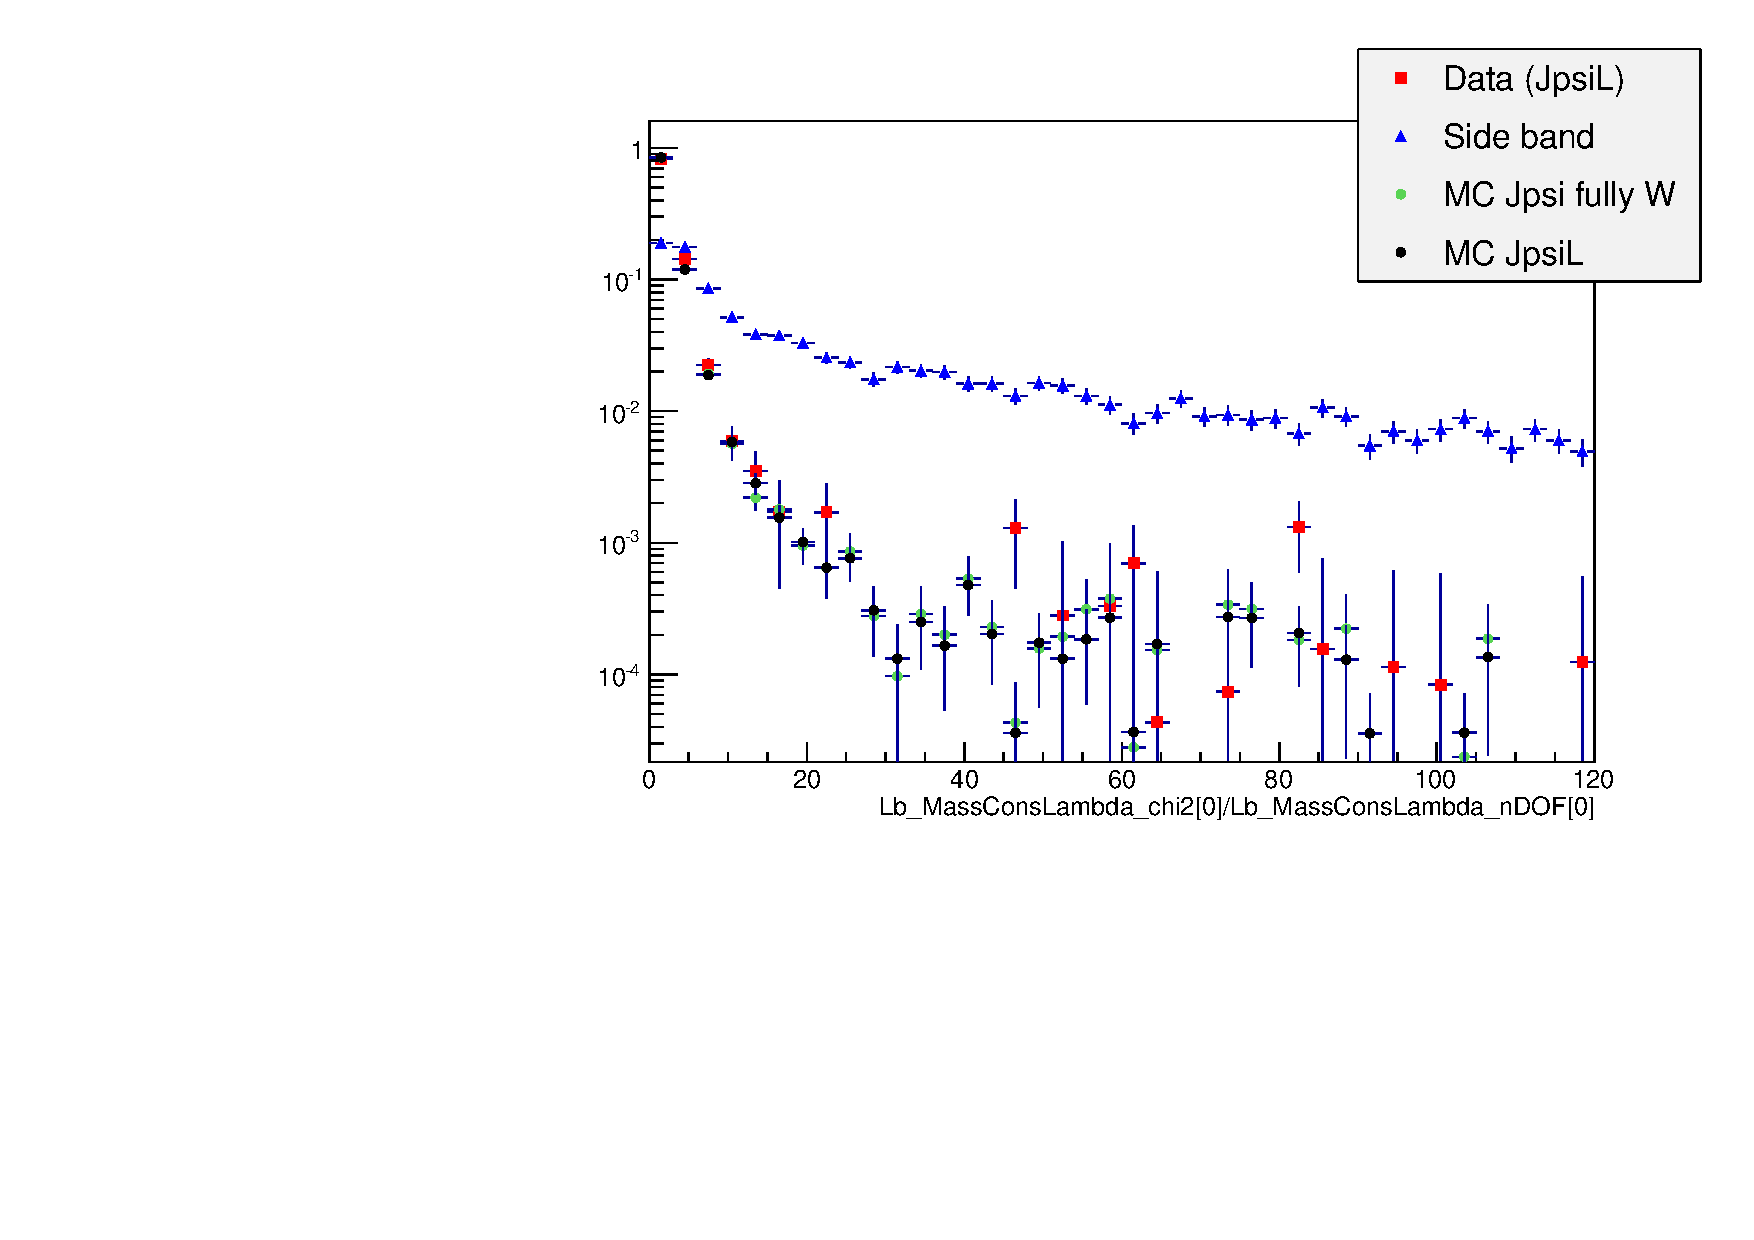
\includegraphics[width=0.48\textwidth]{Lmumu/figs/MC_data_comp/Lb_MassConsLambda_chi20Lb_MassConsLambda_nDOF0_plotLL.pdf}
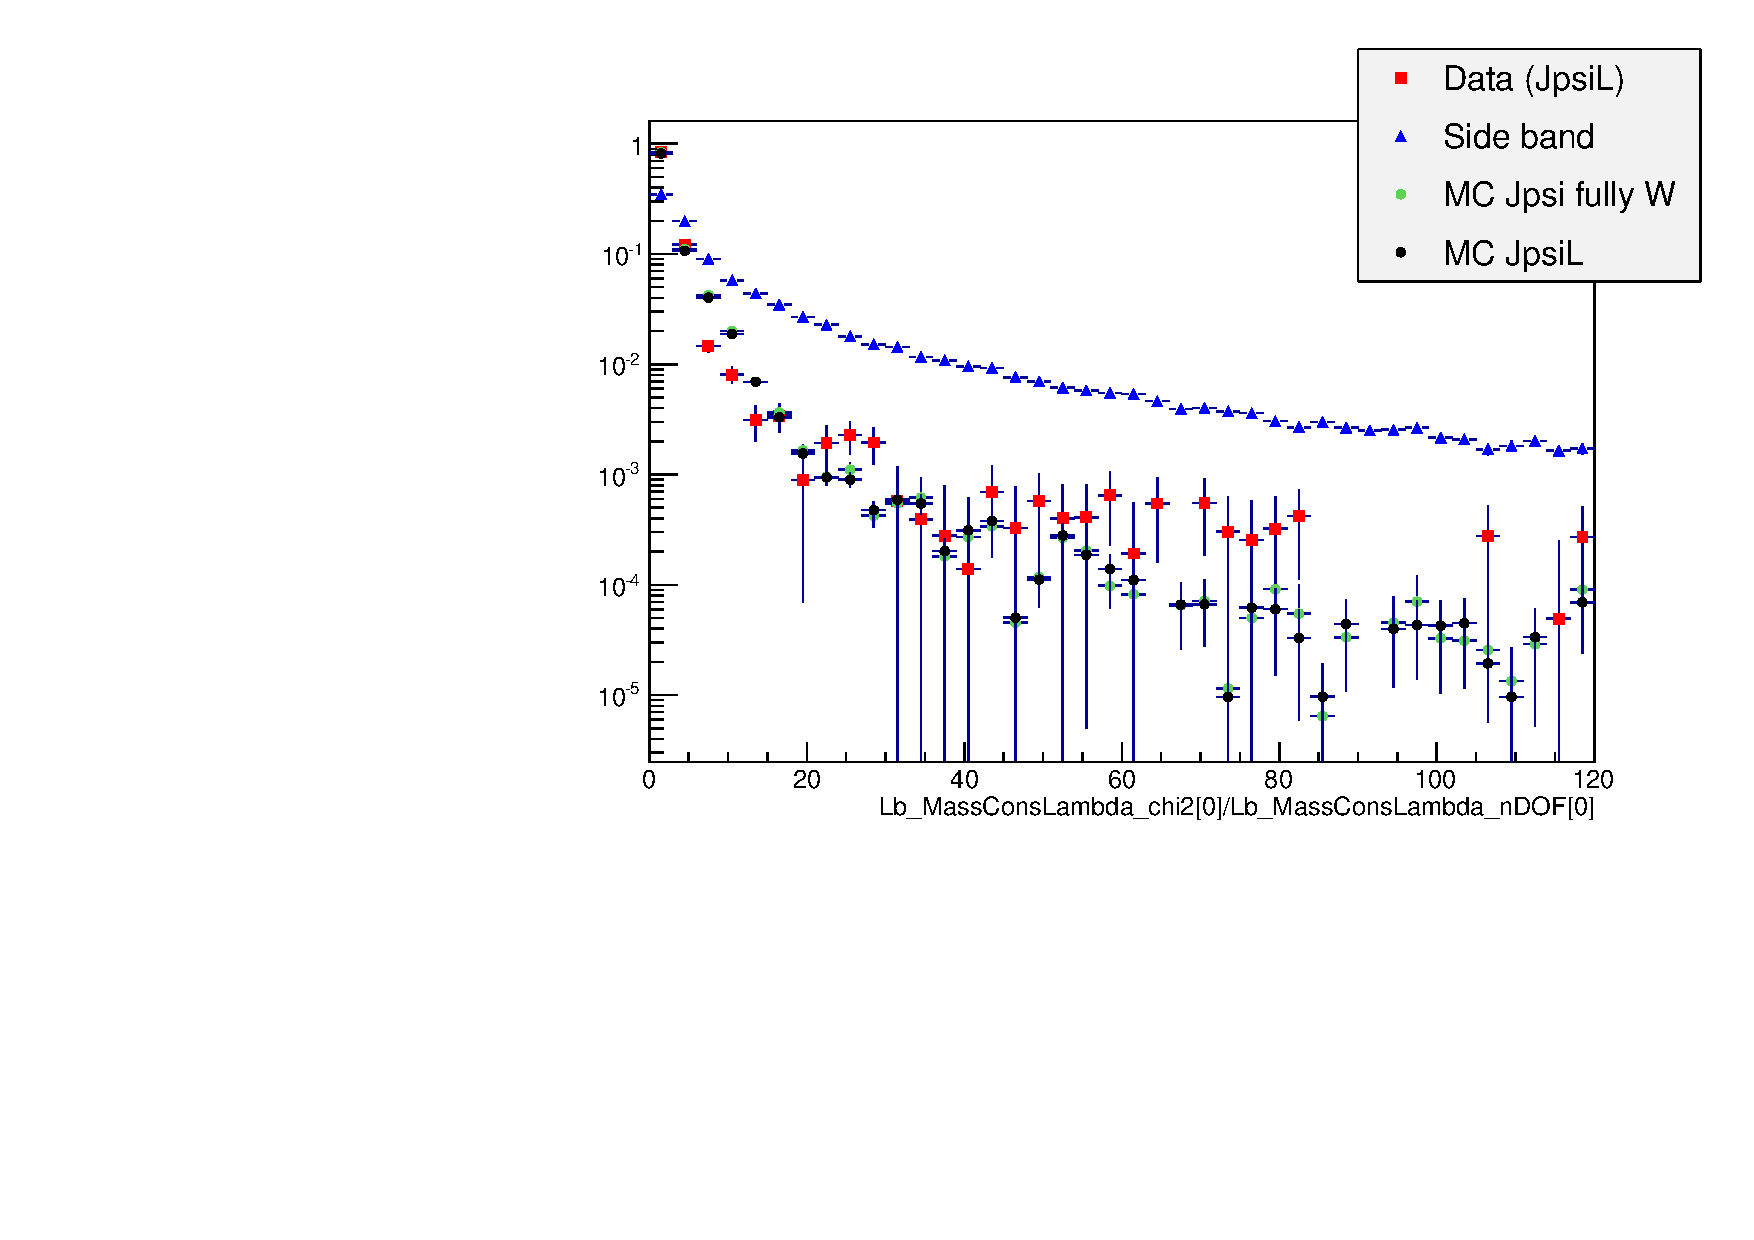
\includegraphics[width=0.48\textwidth]{Lmumu/figs/MC_data_comp/Lb_MassConsLambda_chi20Lb_MassConsLambda_nDOF0_plotDD.pdf}
\caption{ Distributions of $\chi^2/NdF$ of the kinematic fit in data and simulation for LL (left) and DD (right) events.   }
\end{figure}


\begin{figure}[h!]
\centering
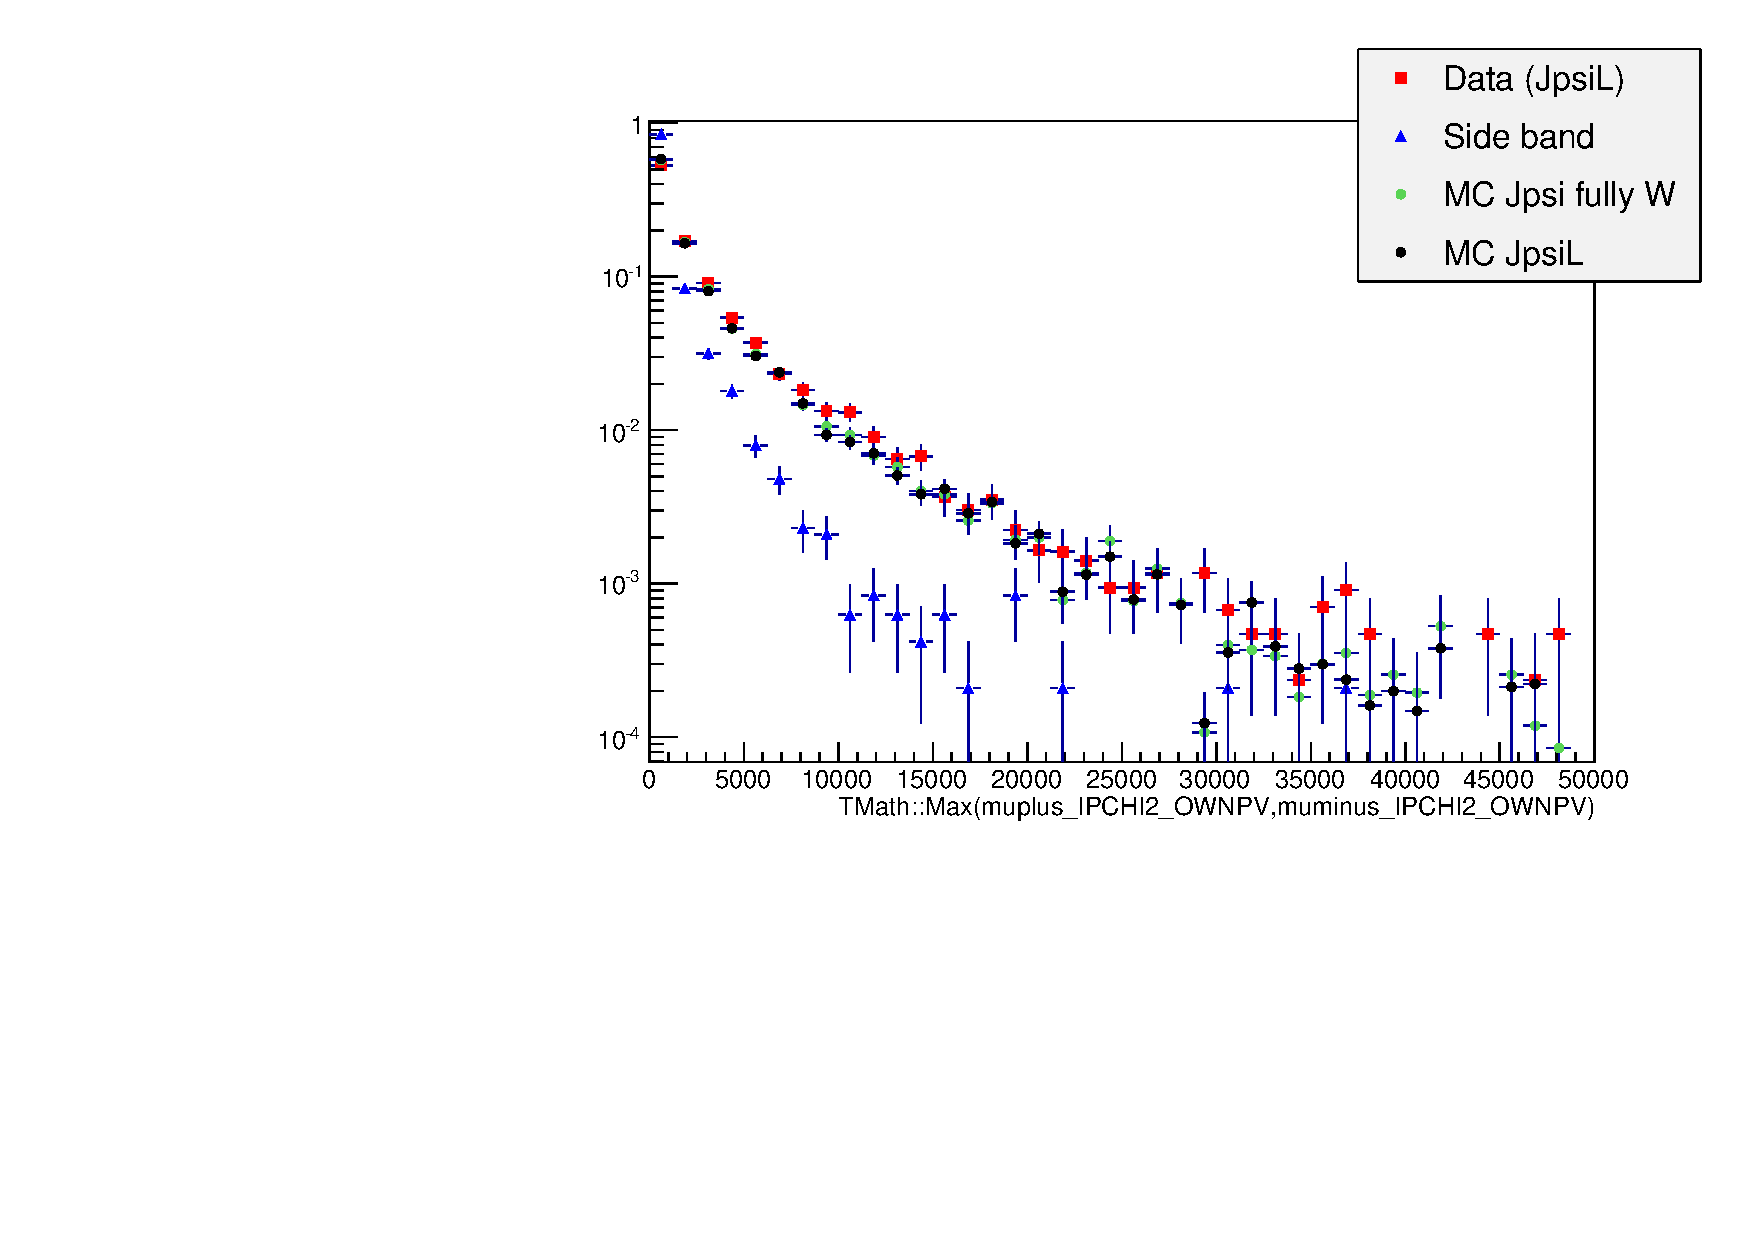
\includegraphics[width=0.48\textwidth]{Lmumu/figs/MC_data_comp/Maxmuplus_IPCHI2_OWNPVmuminus_IPCHI2_OWNPV_plotLL.pdf}
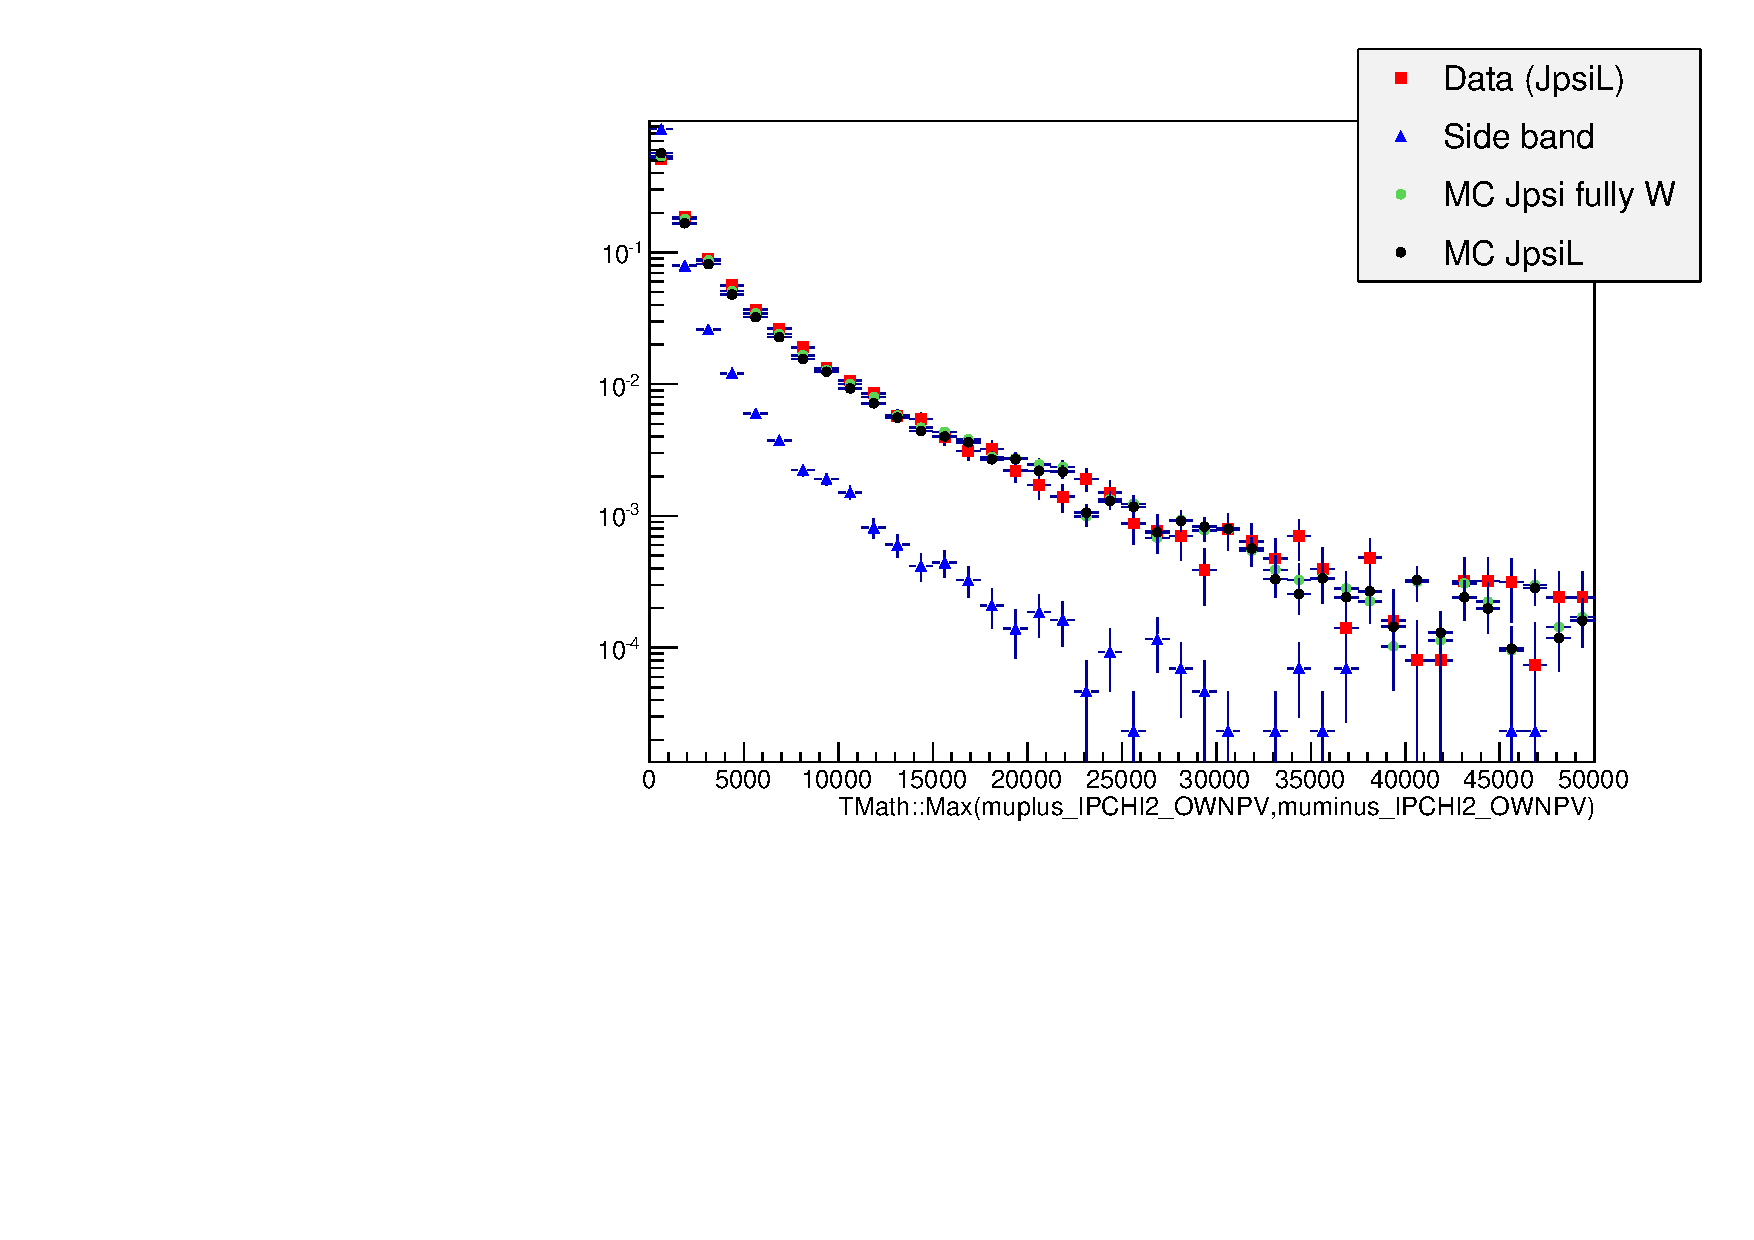
\includegraphics[width=0.48\textwidth]{Lmumu/figs/MC_data_comp/Maxmuplus_IPCHI2_OWNPVmuminus_IPCHI2_OWNPV_plotDD.pdf}
\caption{ Distributions of maximum muon $IP\chi^2$ variable in data and simulation for LL (left) and DD (right) events.   }
\end{figure}

%\begin{figure}[h!]
%\centering
%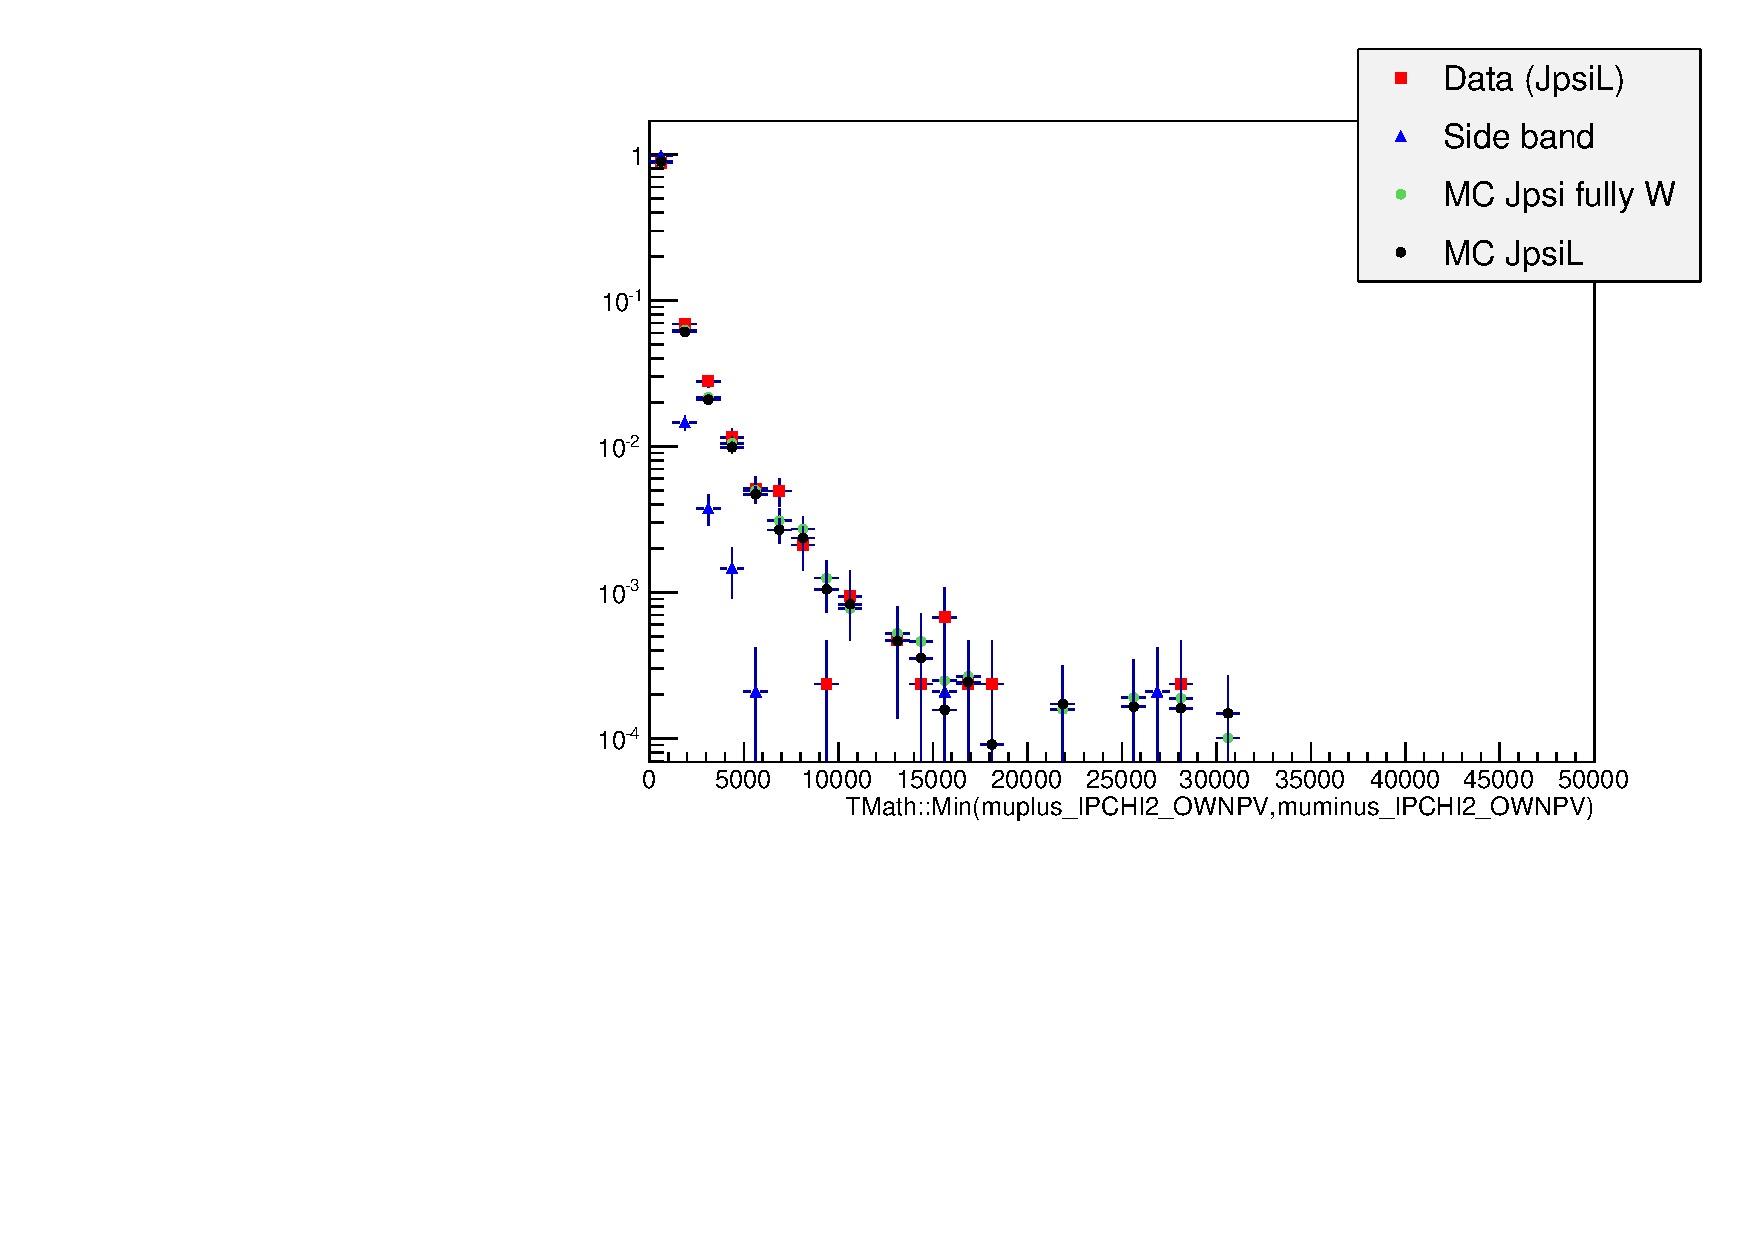
\includegraphics[width=0.48\textwidth]{Lmumu/figs/MC_data_comp/Minmuplus_IPCHI2_OWNPVmuminus_IPCHI2_OWNPV_plotLL.pdf}
%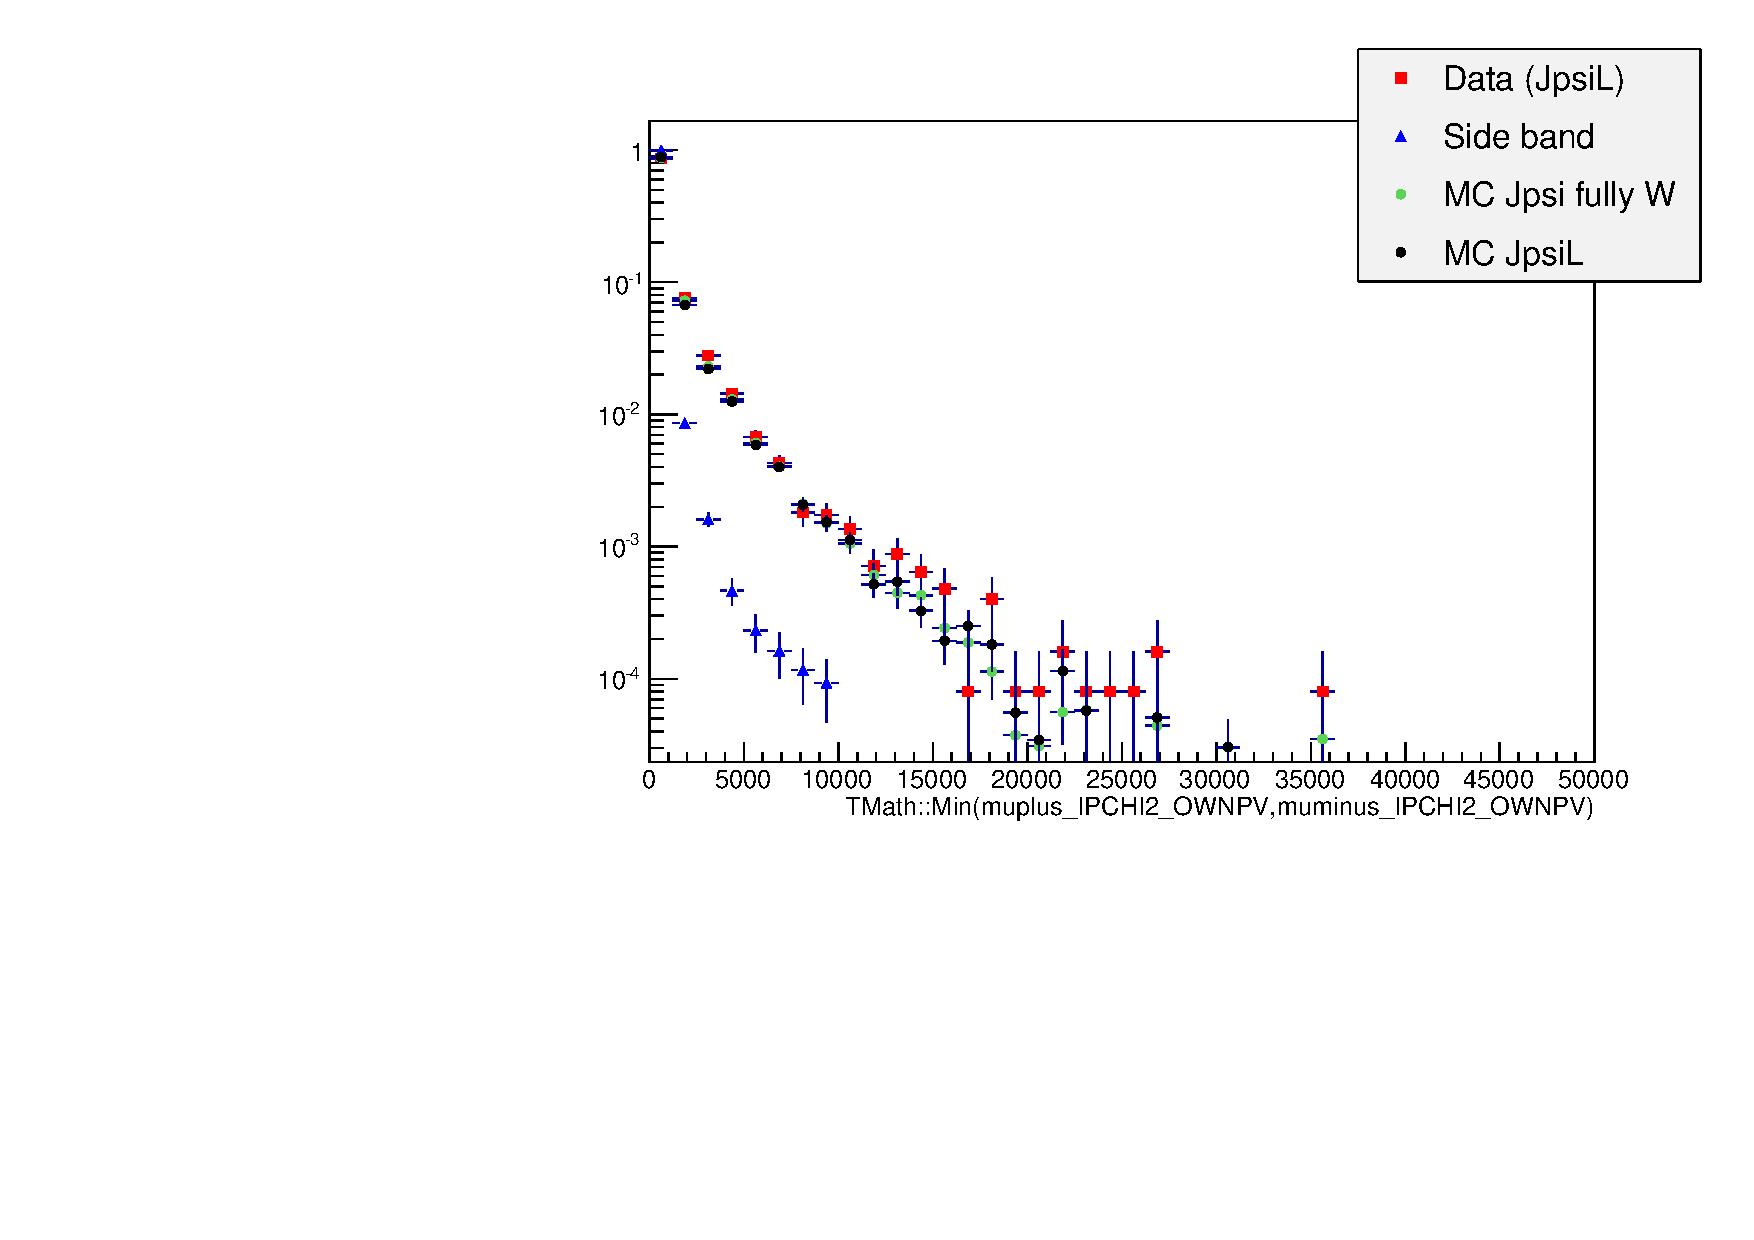
\includegraphics[width=0.48\textwidth]{Lmumu/figs/MC_data_comp/Minmuplus_IPCHI2_OWNPVmuminus_IPCHI2_OWNPV_plotDD.pdf}
%\caption{ Distributions of minimum muon $IP\chi^2$ variable in data and simulation for LL (left) and DD (right) events.   }
%\end{figure}

%\begin{figure}[h!]
%\centering
%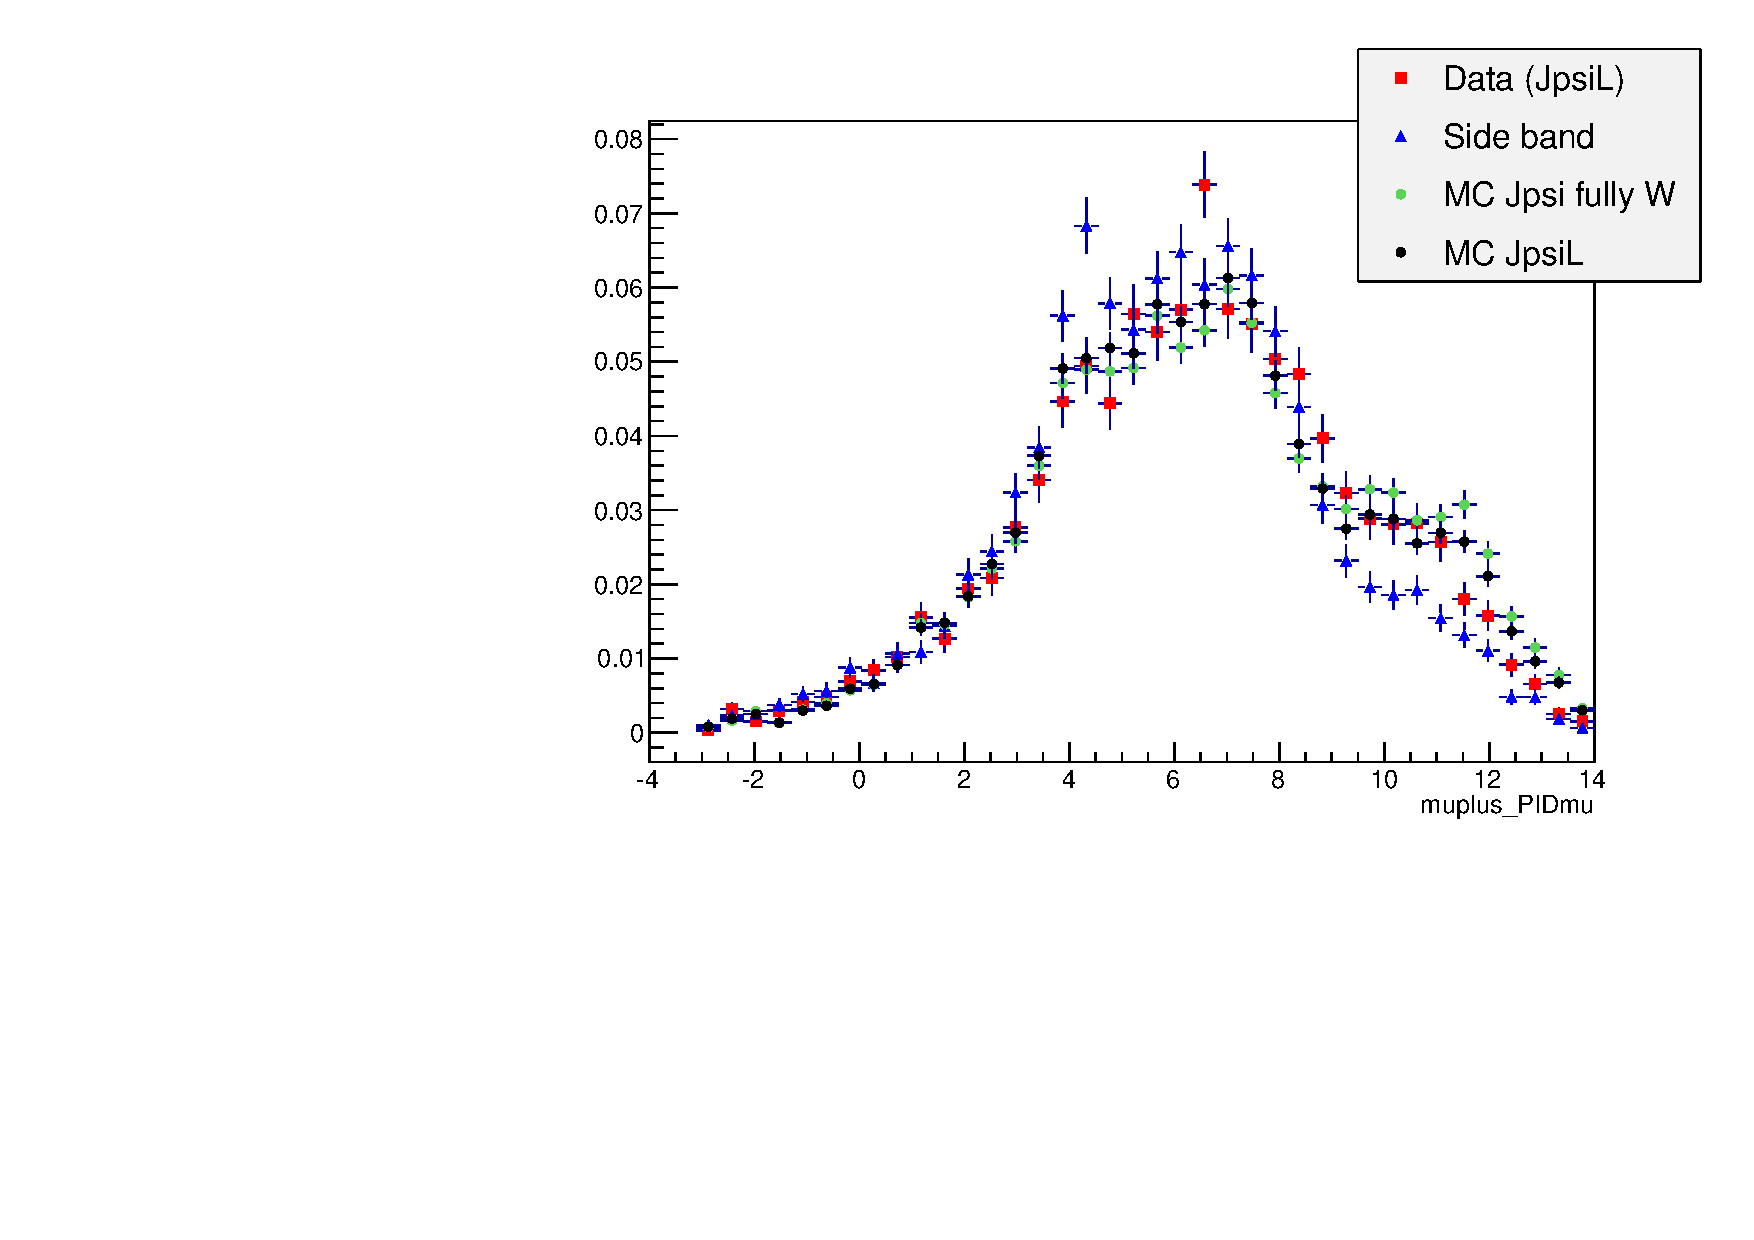
\includegraphics[width=0.48\textwidth]{Lmumu/figs/MC_data_comp/muplus_PIDmu_plotLL.pdf}
%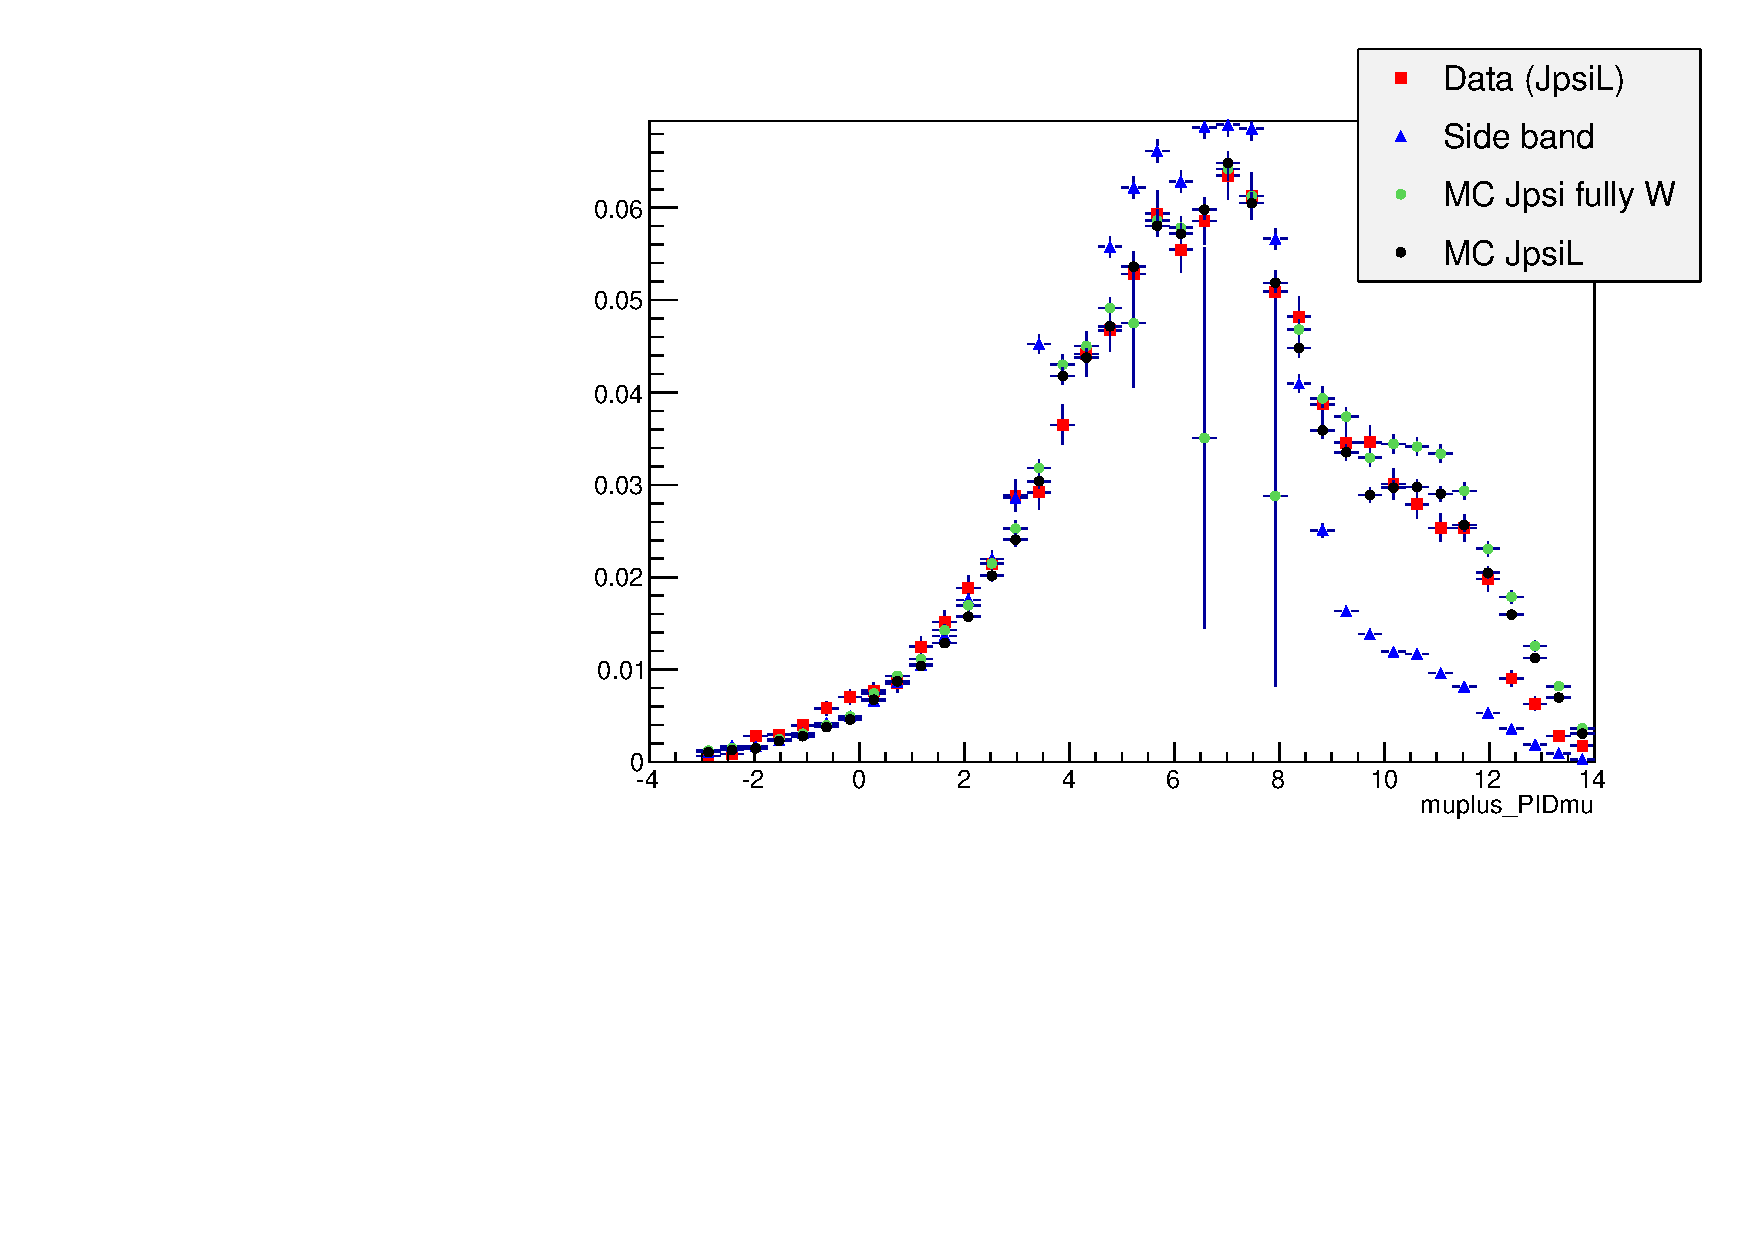
\includegraphics[width=0.48\textwidth]{Lmumu/figs/MC_data_comp/muplus_PIDmu_plotDD.pdf}
%\caption{ Distributions of muon PID using the DLL variable in data and simulation for LL (left) and DD (right) events.   }
%\end{figure}



%\begin{figure}[h!]
%\centering
%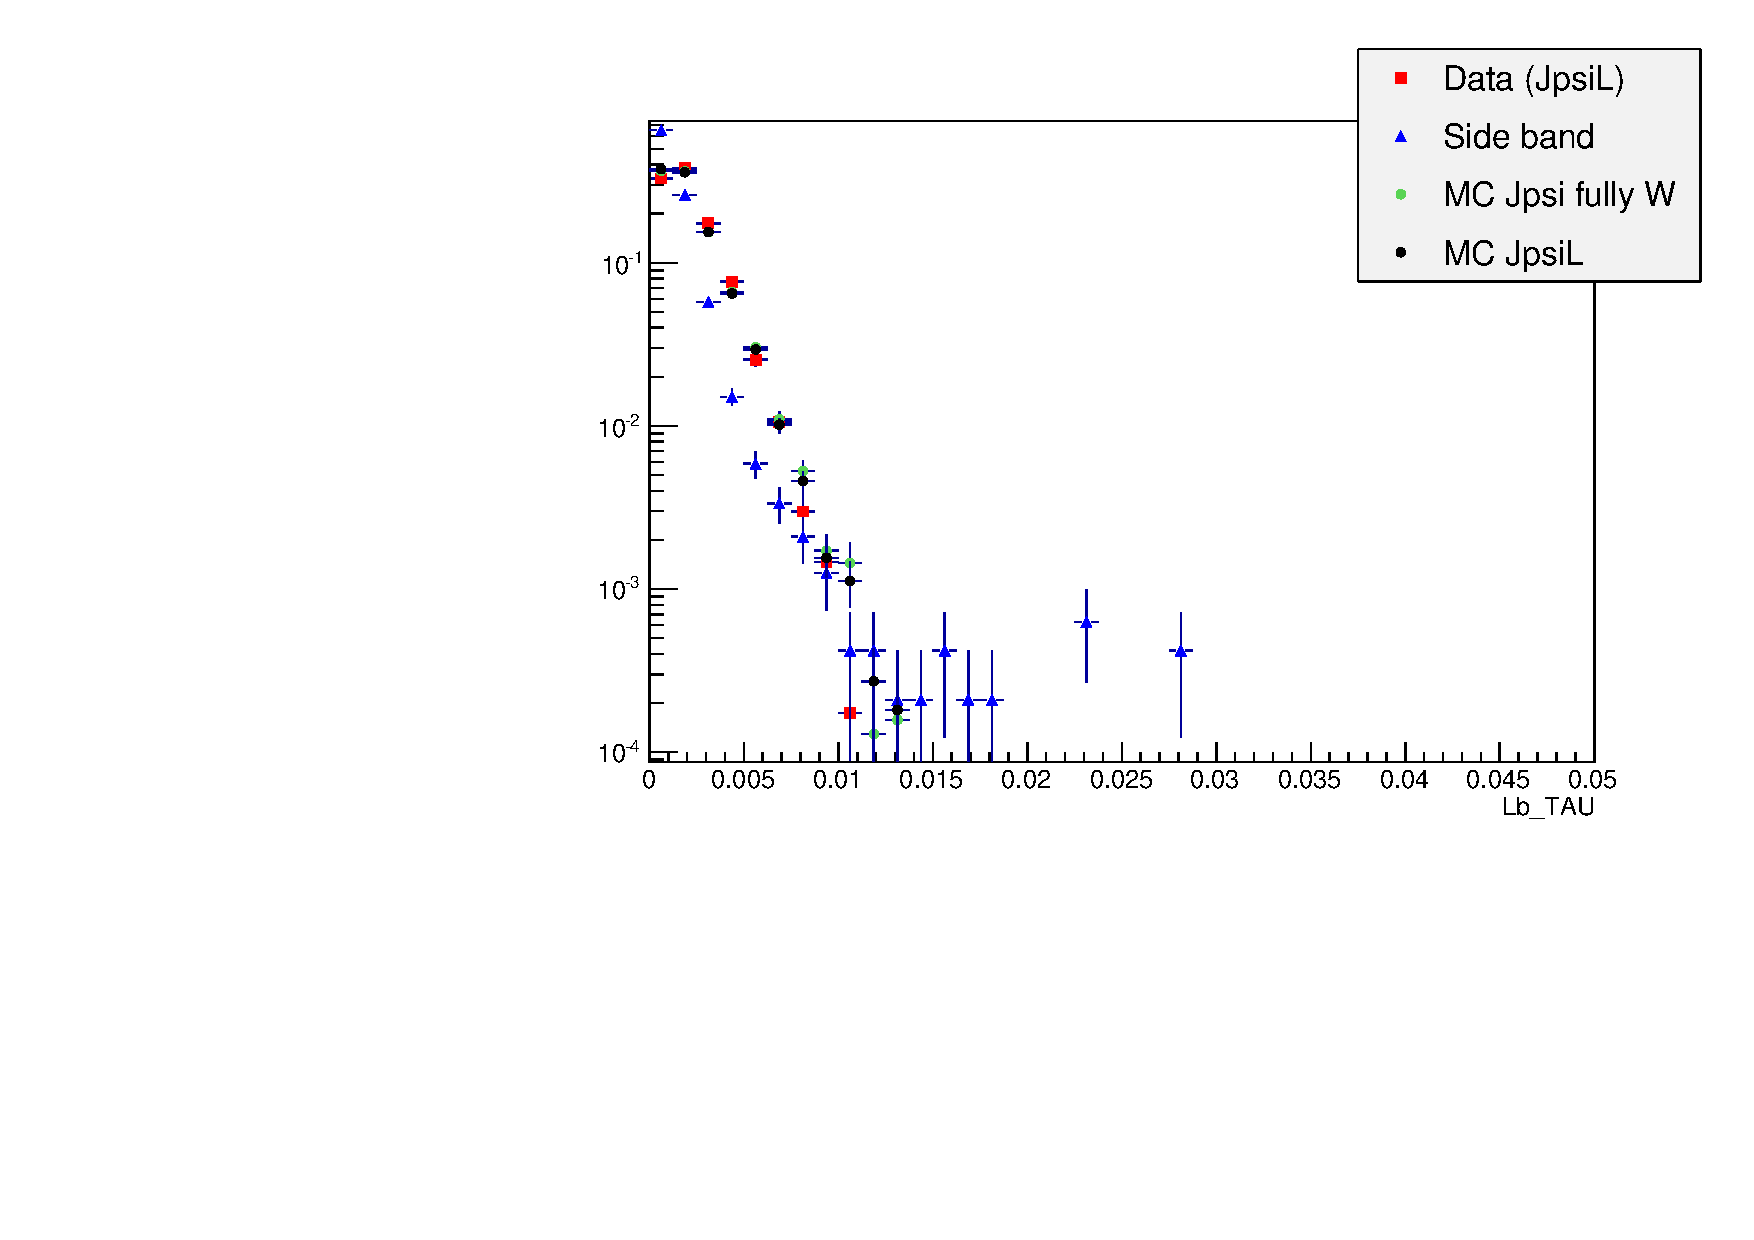
\includegraphics[width=0.48\textwidth]{Lmumu/figs/MC_data_comp/Lb_TAU_plotLL.pdf}
%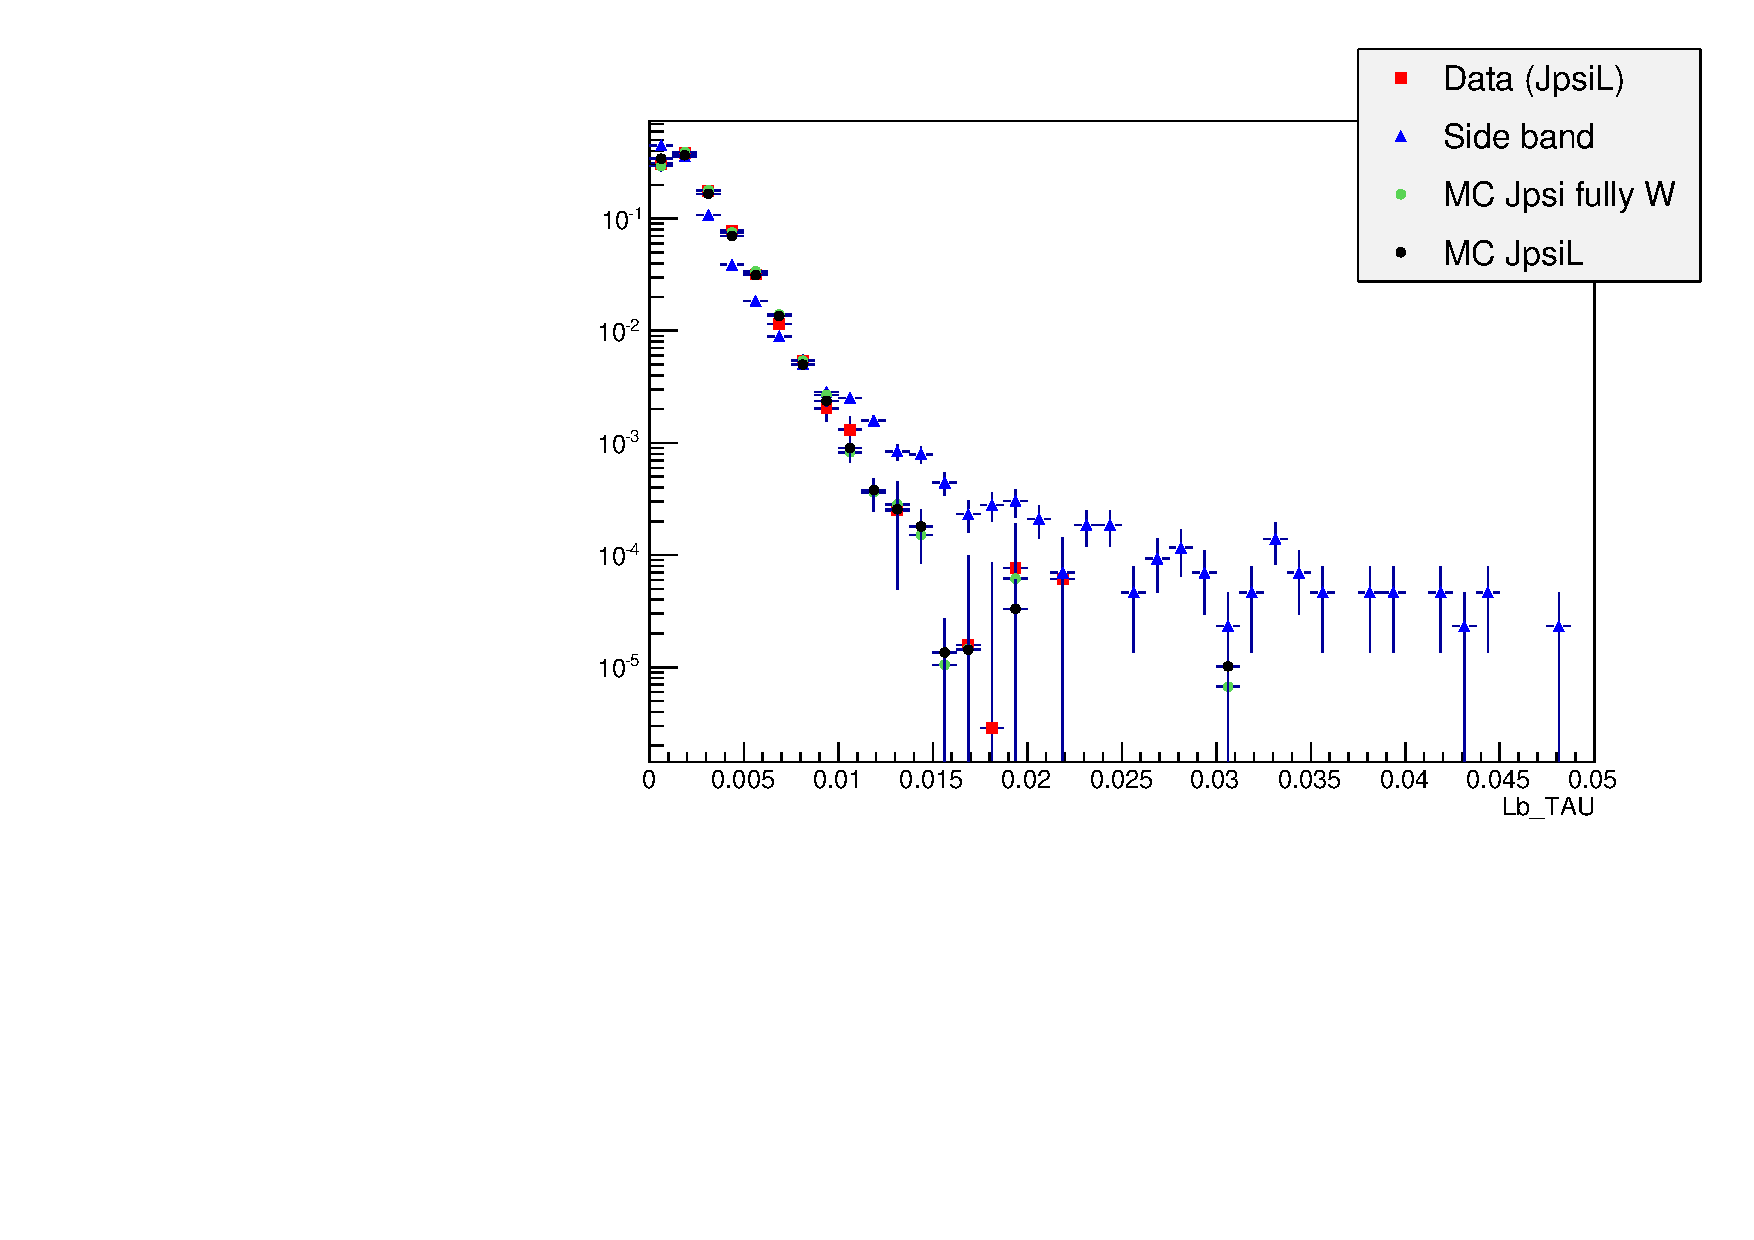
\includegraphics[width=0.48\textwidth]{Lmumu/figs/MC_data_comp/Lb_TAU_plotDD.pdf}
%\caption{ Distributions of \Lb lifetime variable in MC, data signal and data background for LL (left) and DD (right) events.   }
%\end{figure}



\begin{figure}[h!]
\centering
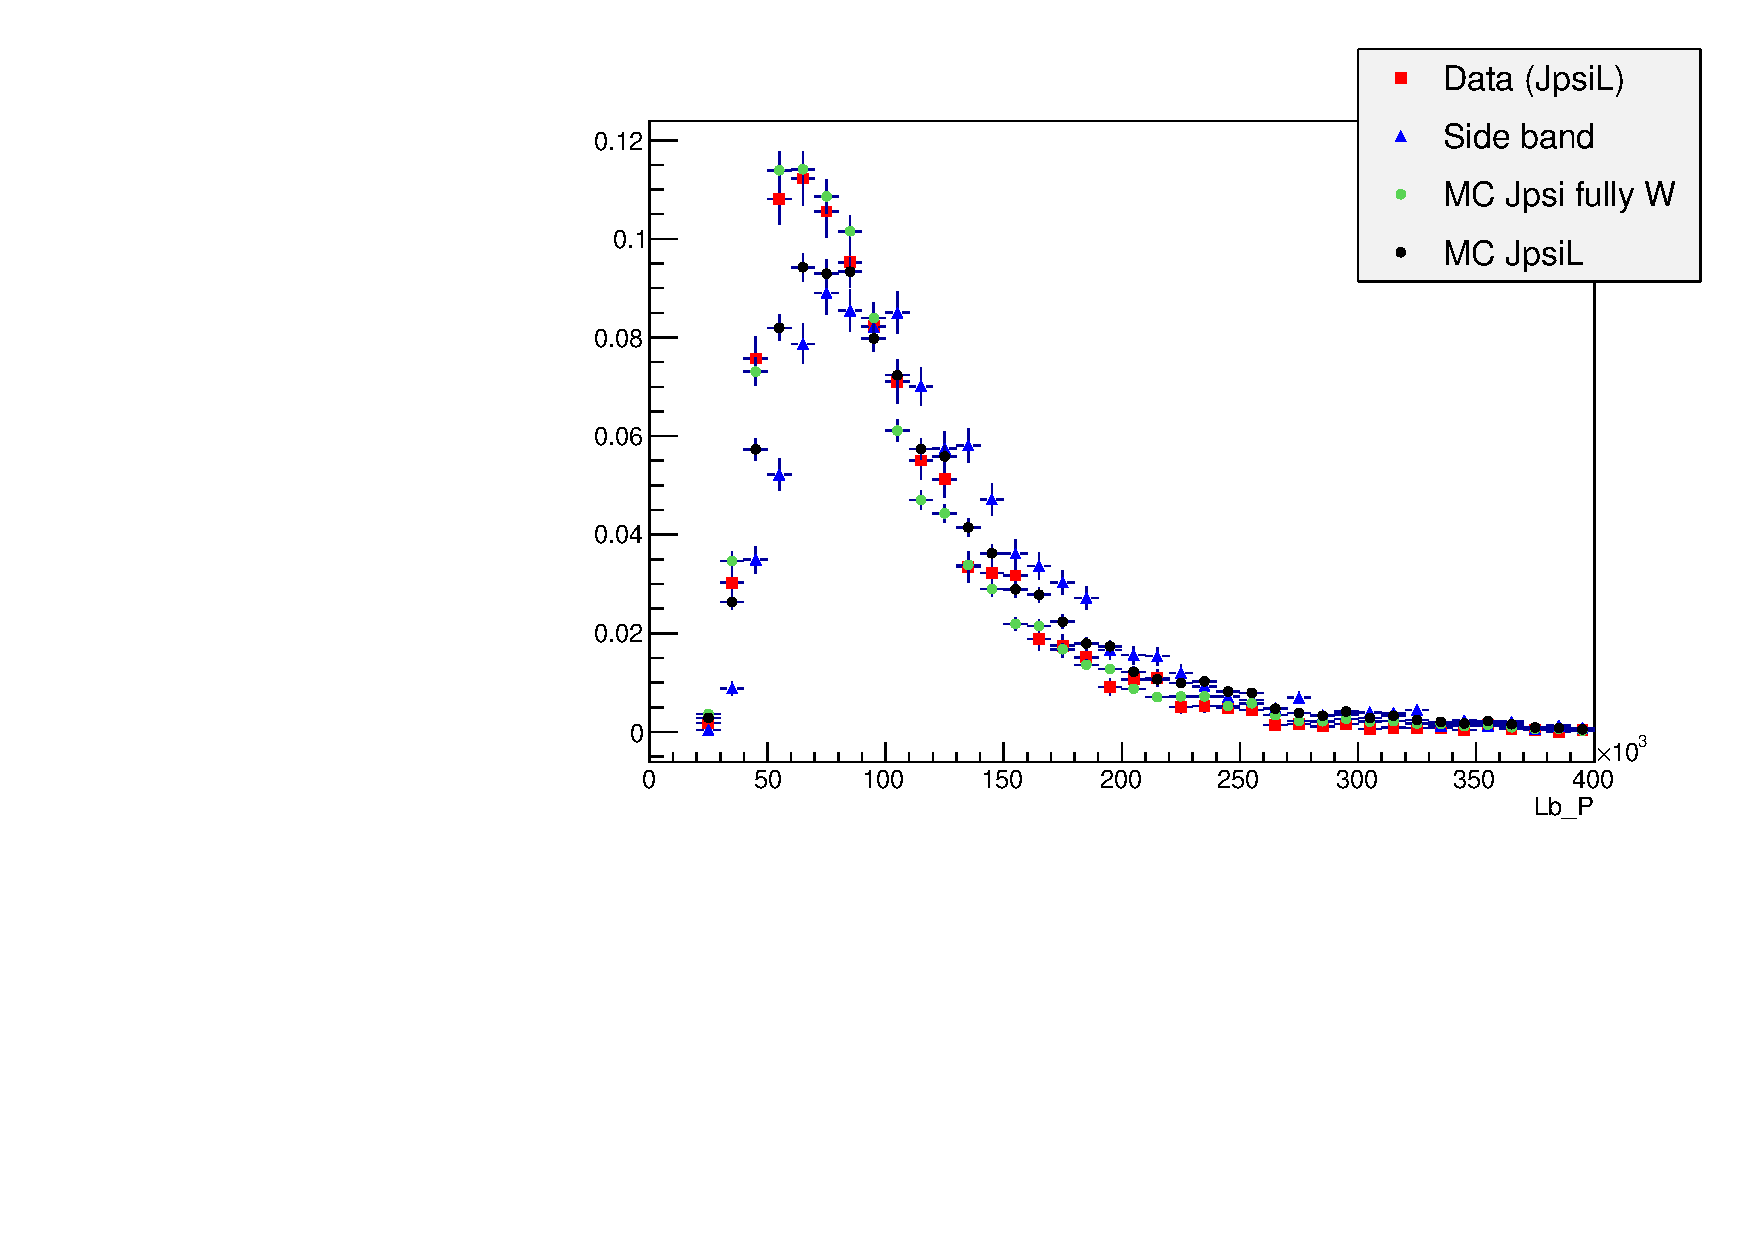
\includegraphics[width=0.48\textwidth]{Lmumu/figs/MC_data_comp/Lb_P_plotLL.pdf}
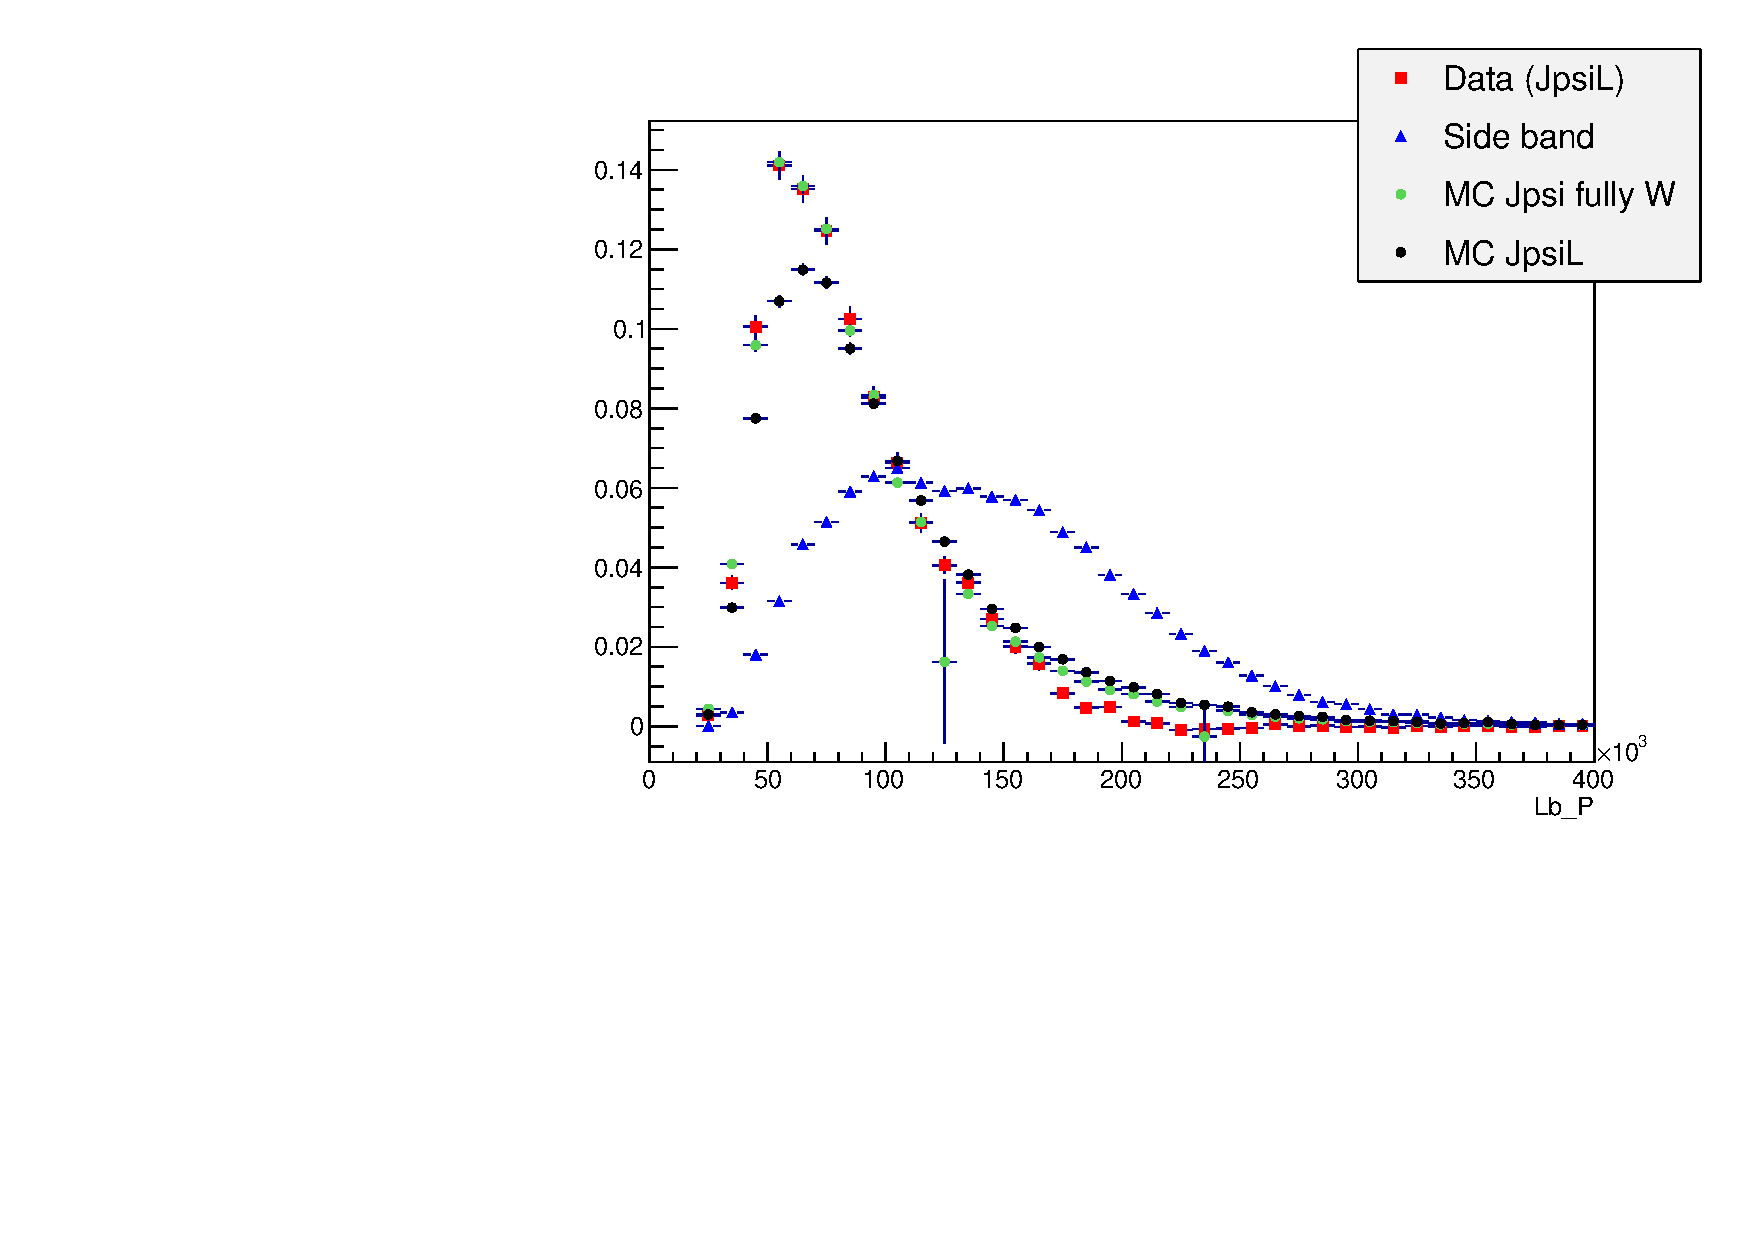
\includegraphics[width=0.48\textwidth]{Lmumu/figs/MC_data_comp/Lb_P_plotDD.pdf}
\caption{ Distributions of \Lb momentum variable in data and simulation for LL (left) and DD (right) events.   }
\end{figure}

%\begin{figure}[h!]
%\centering
%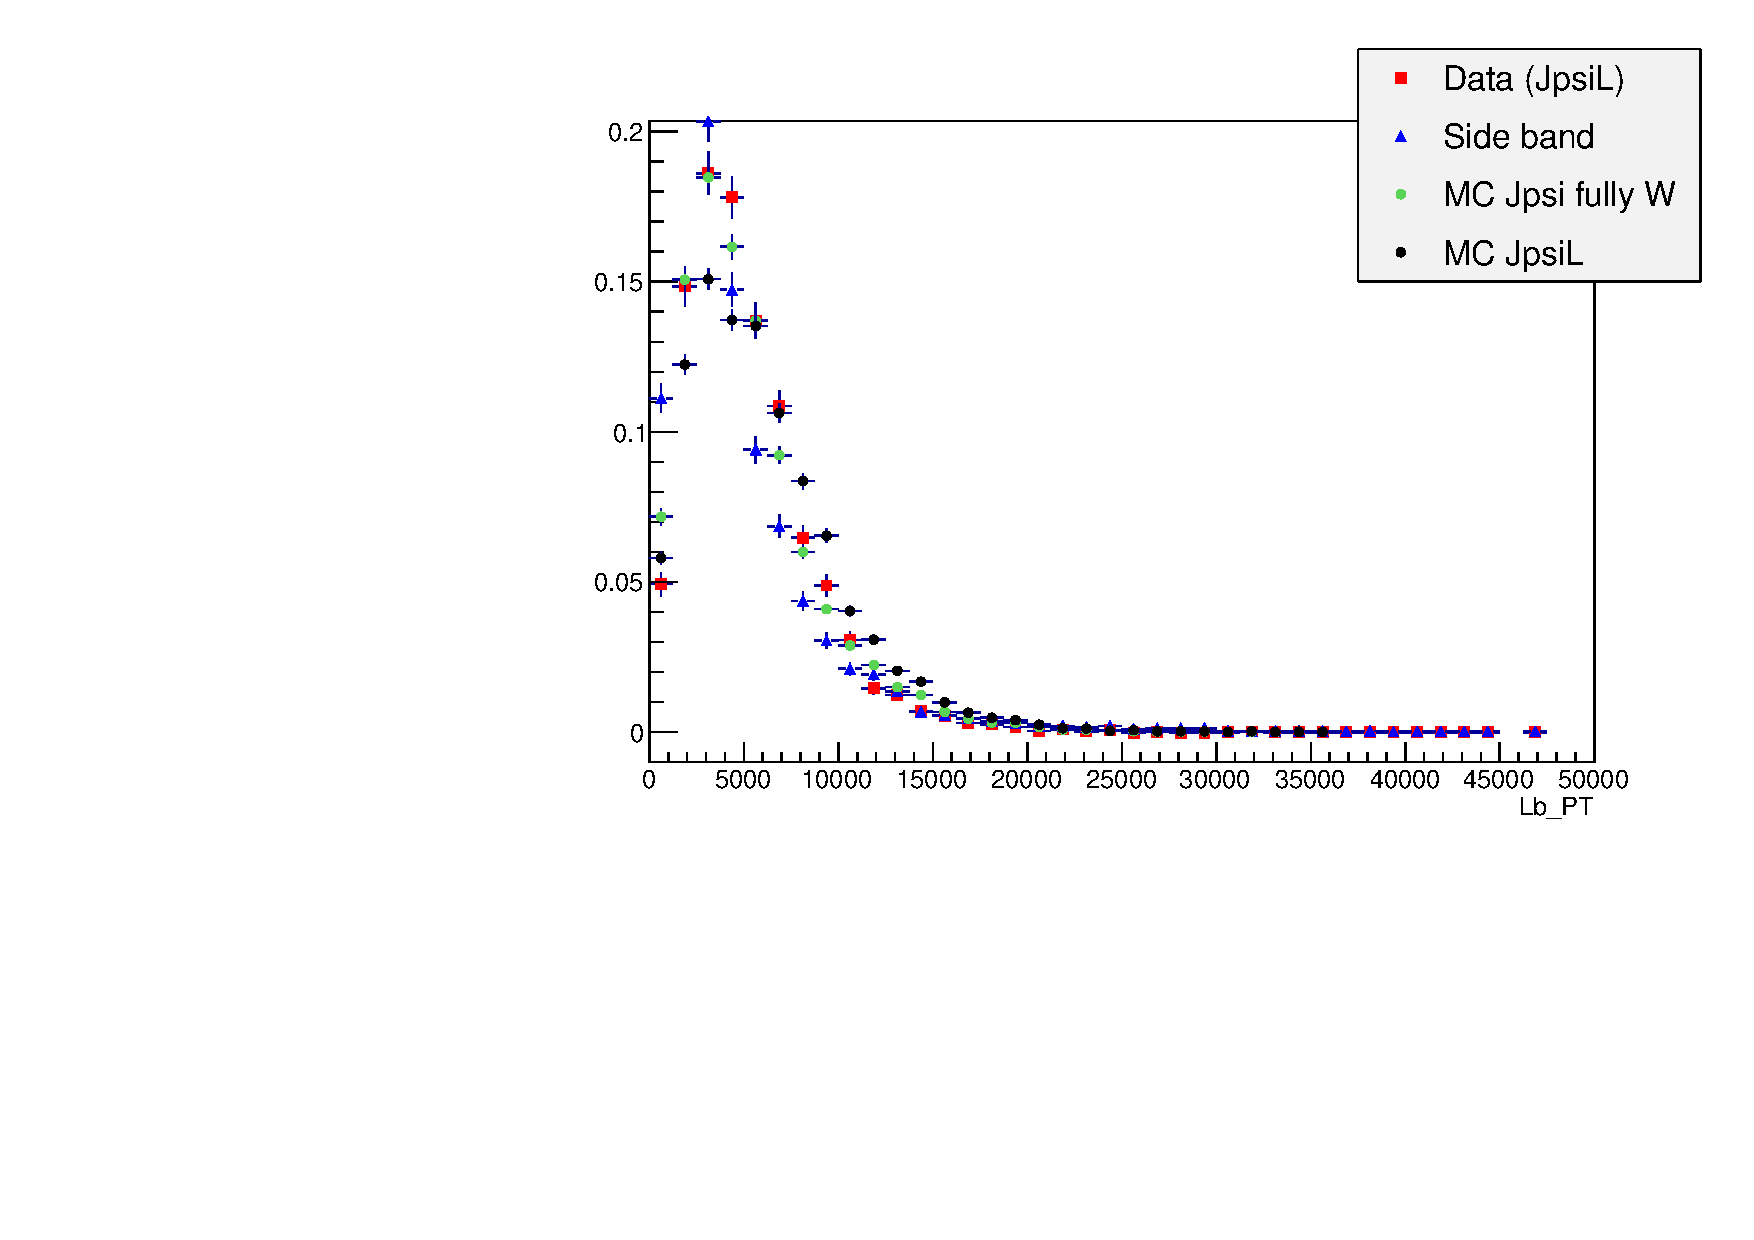
\includegraphics[width=0.48\textwidth]{Lmumu/figs/MC_data_comp/Lb_PT_plotLL.pdf}
%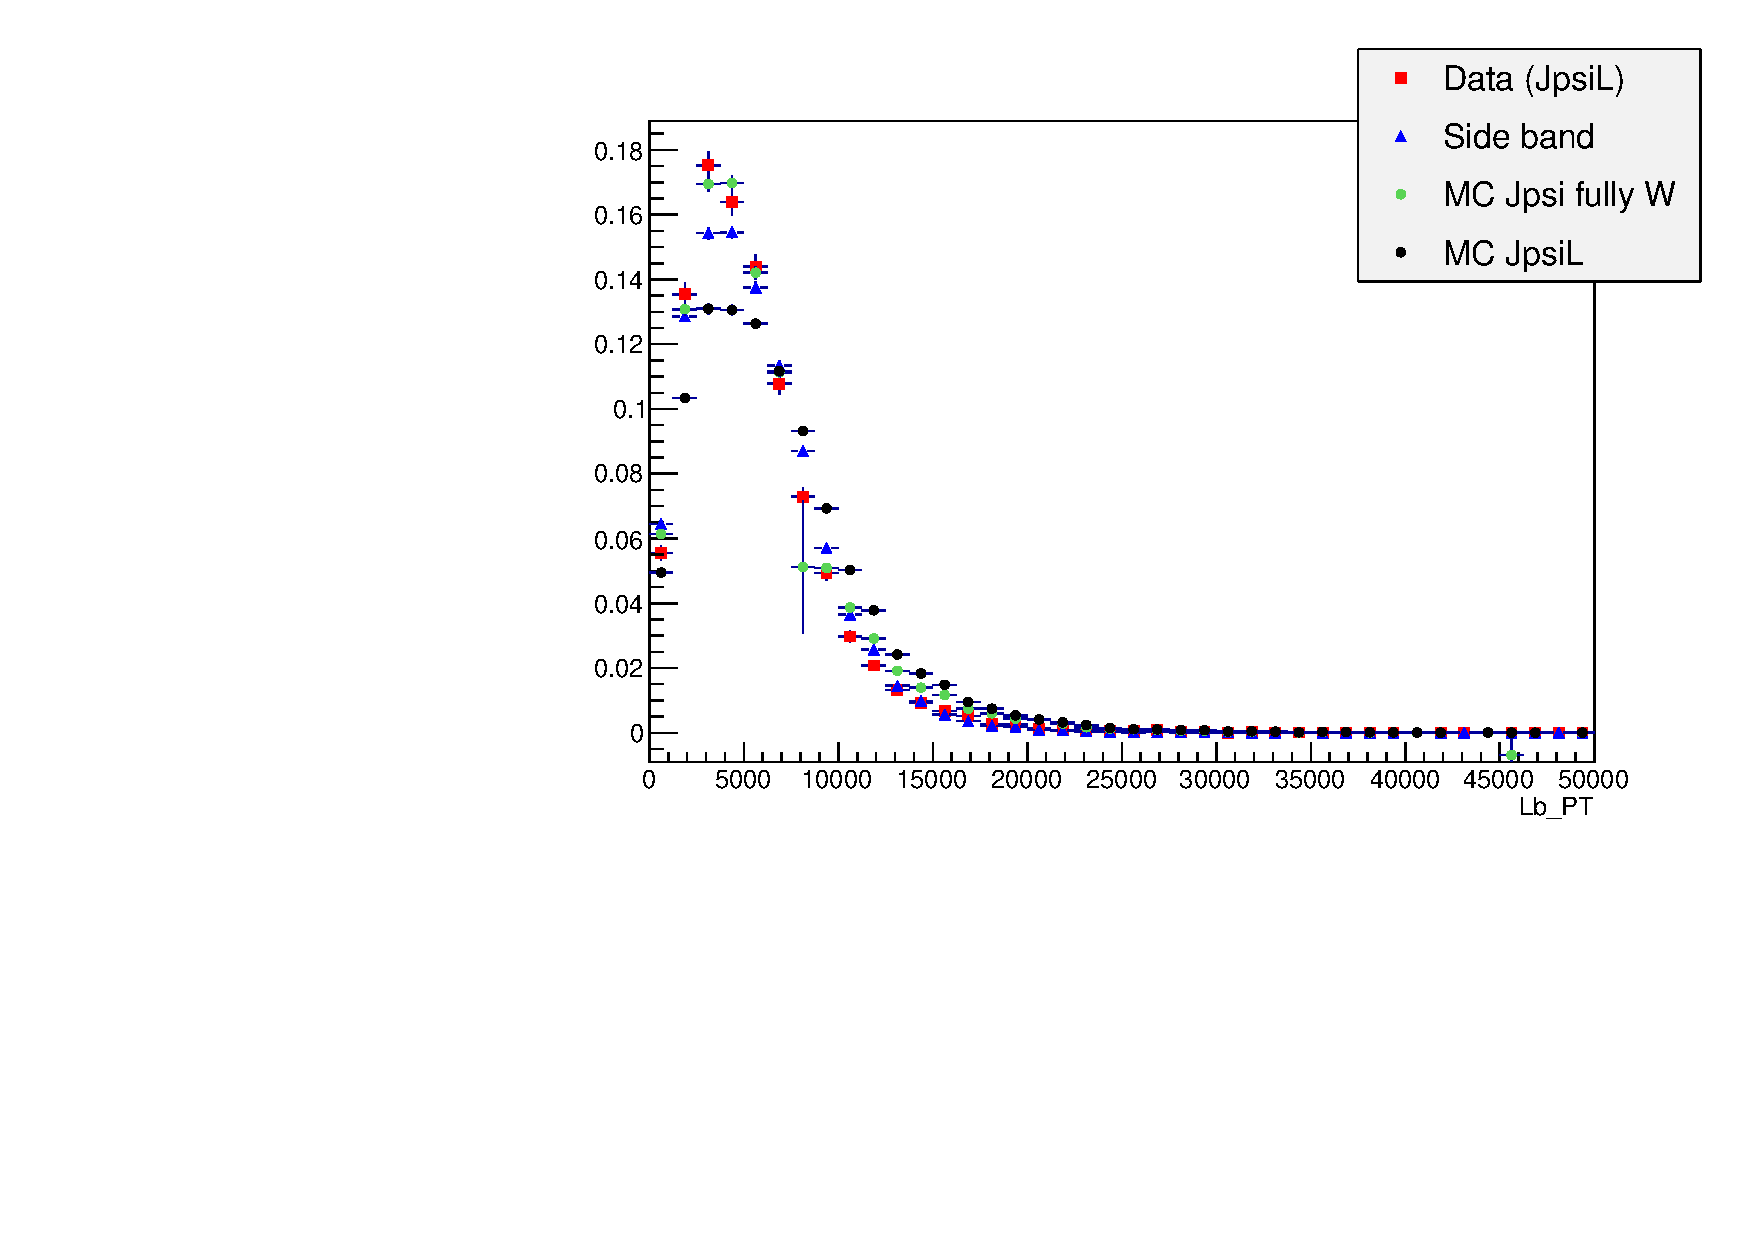
\includegraphics[width=0.48\textwidth]{Lmumu/figs/MC_data_comp/Lb_PT_plotDD.pdf}
%\caption{ Distributions of \Lb trasverse momentum variable in MC, data signal and data background for LL (left) and DD (right) events.   }
%\end{figure}

%\begin{figure}[h!]
%\centering
%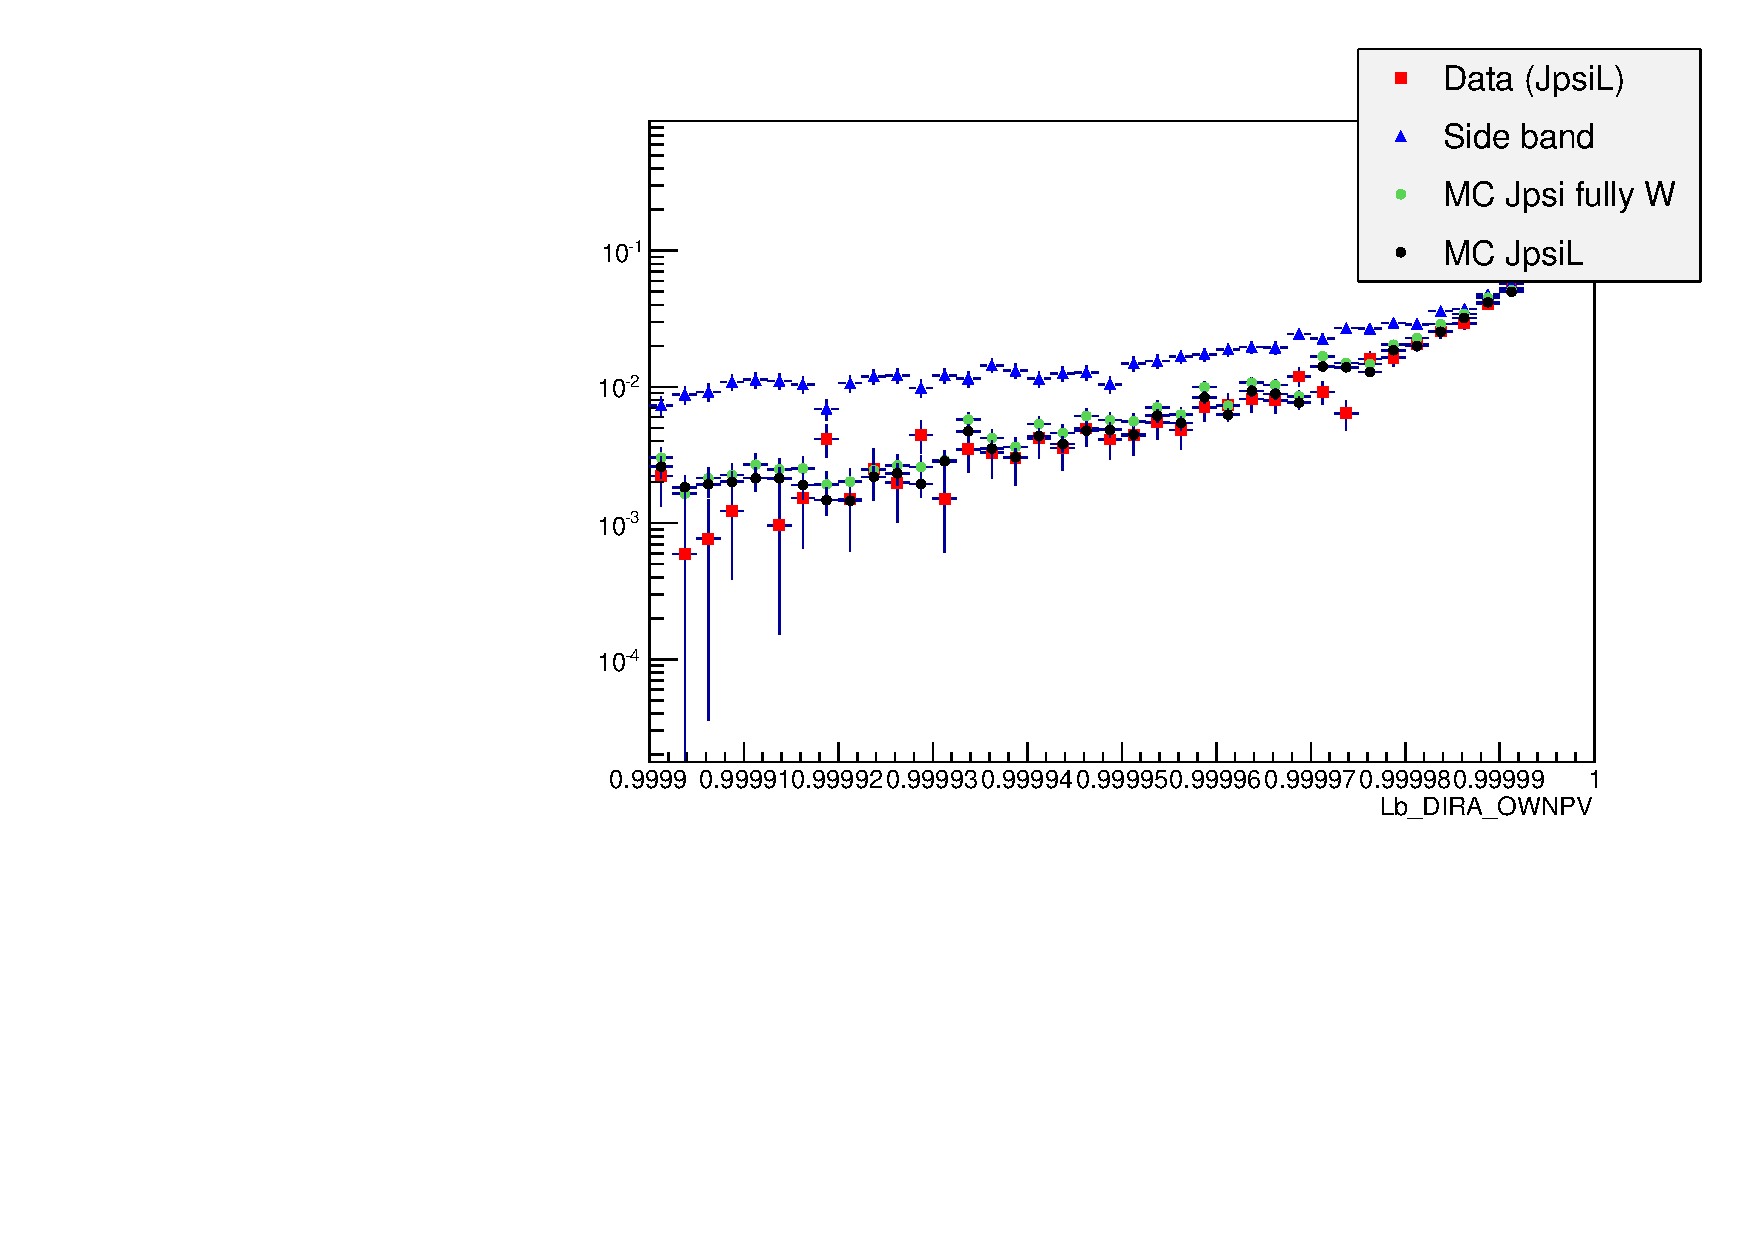
\includegraphics[width=0.48\textwidth]{Lmumu/figs/MC_data_comp/Lb_DIRA_OWNPV_plotLL.pdf}
%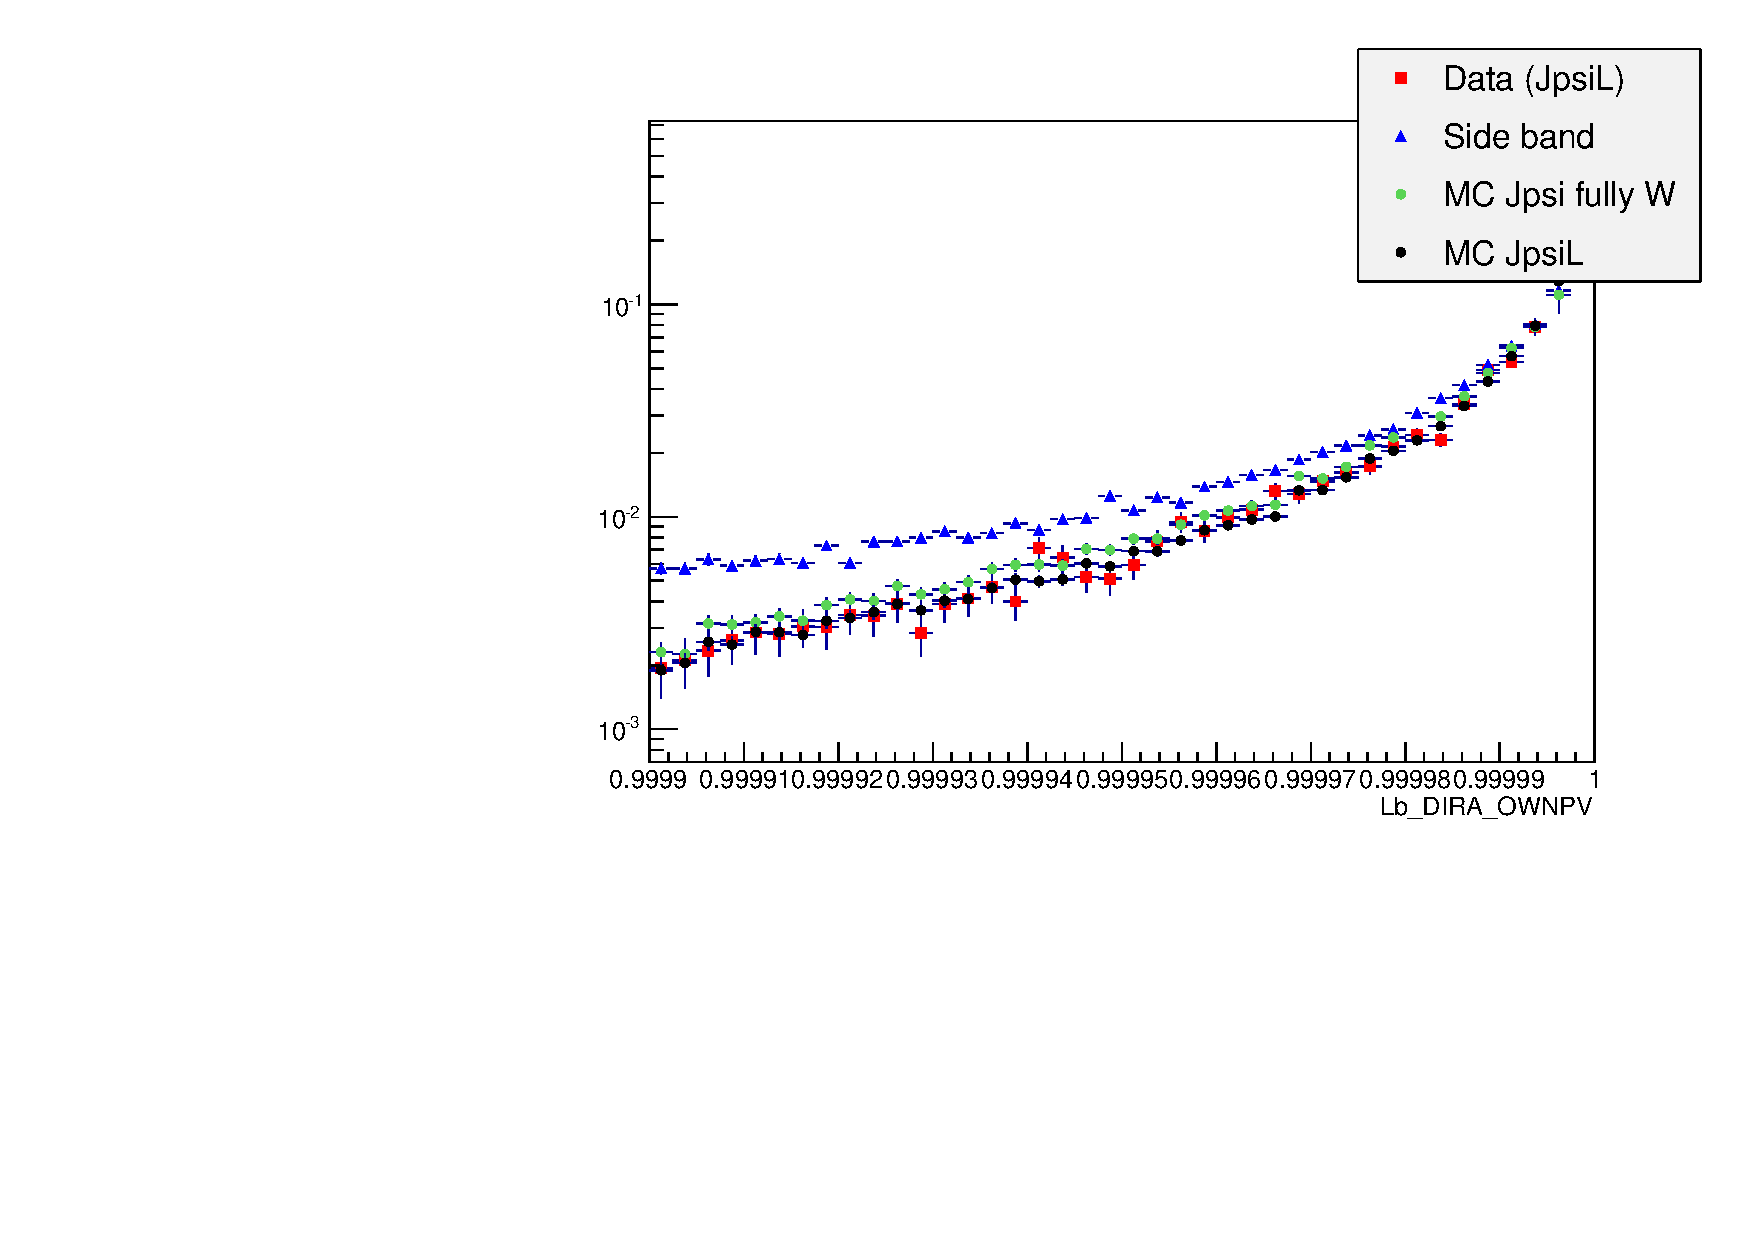
\includegraphics[width=0.48\textwidth]{Lmumu/figs/MC_data_comp/Lb_DIRA_OWNPV_plotDD.pdf}
%\caption{ Distributions of \Lb DIRA variable in MC, data signal and data background for LL (left) and DD (right) events.   }
%\end{figure}

\begin{figure}[h!]
\centering
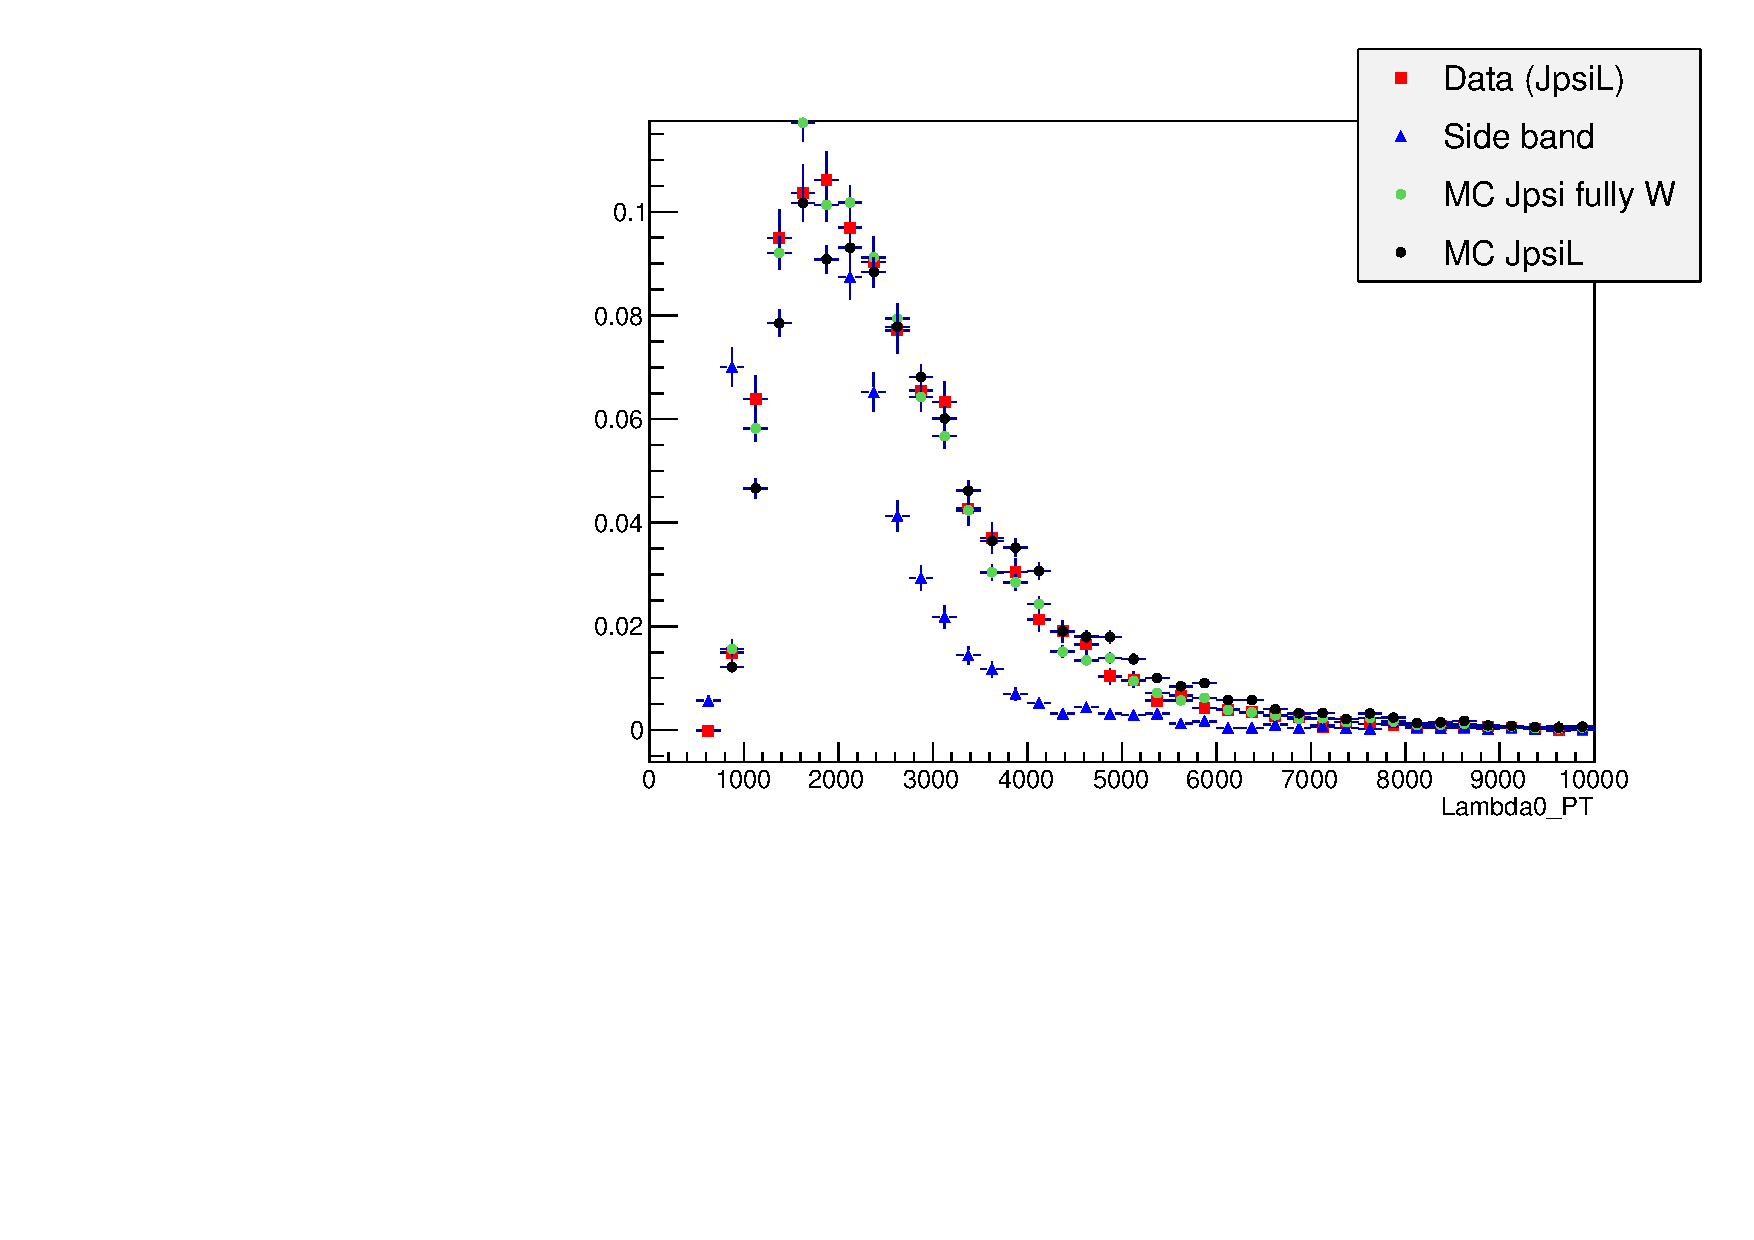
\includegraphics[width=0.48\textwidth]{Lmumu/figs/MC_data_comp/Lambda0_PT_plotLL.pdf}
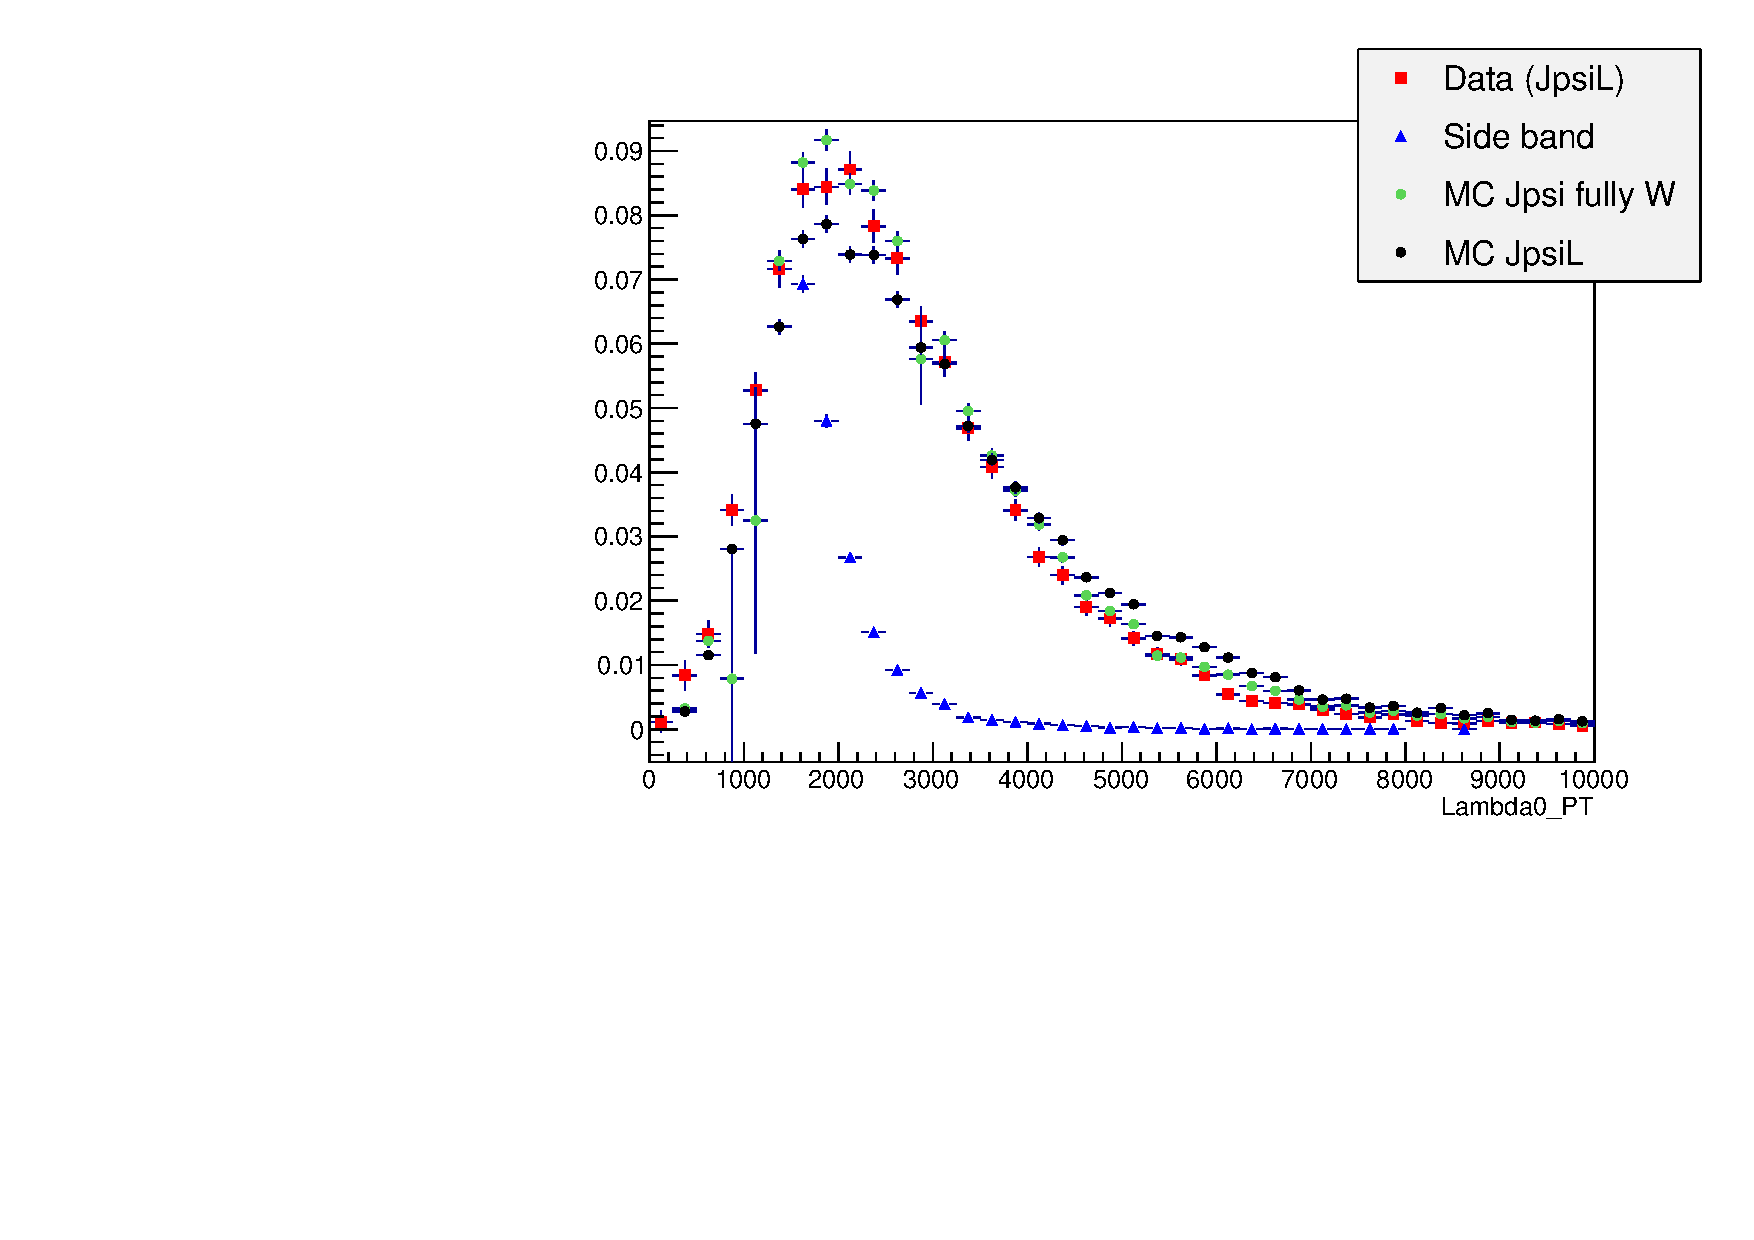
\includegraphics[width=0.48\textwidth]{Lmumu/figs/MC_data_comp/Lambda0_PT_plotDD.pdf}
\caption{ Distributions of \Lz transverse momentum variable in MC, data signal and data background for LL (left) and DD (right) events.   }
\end{figure}


%\begin{figure}[h!]
%\centering
%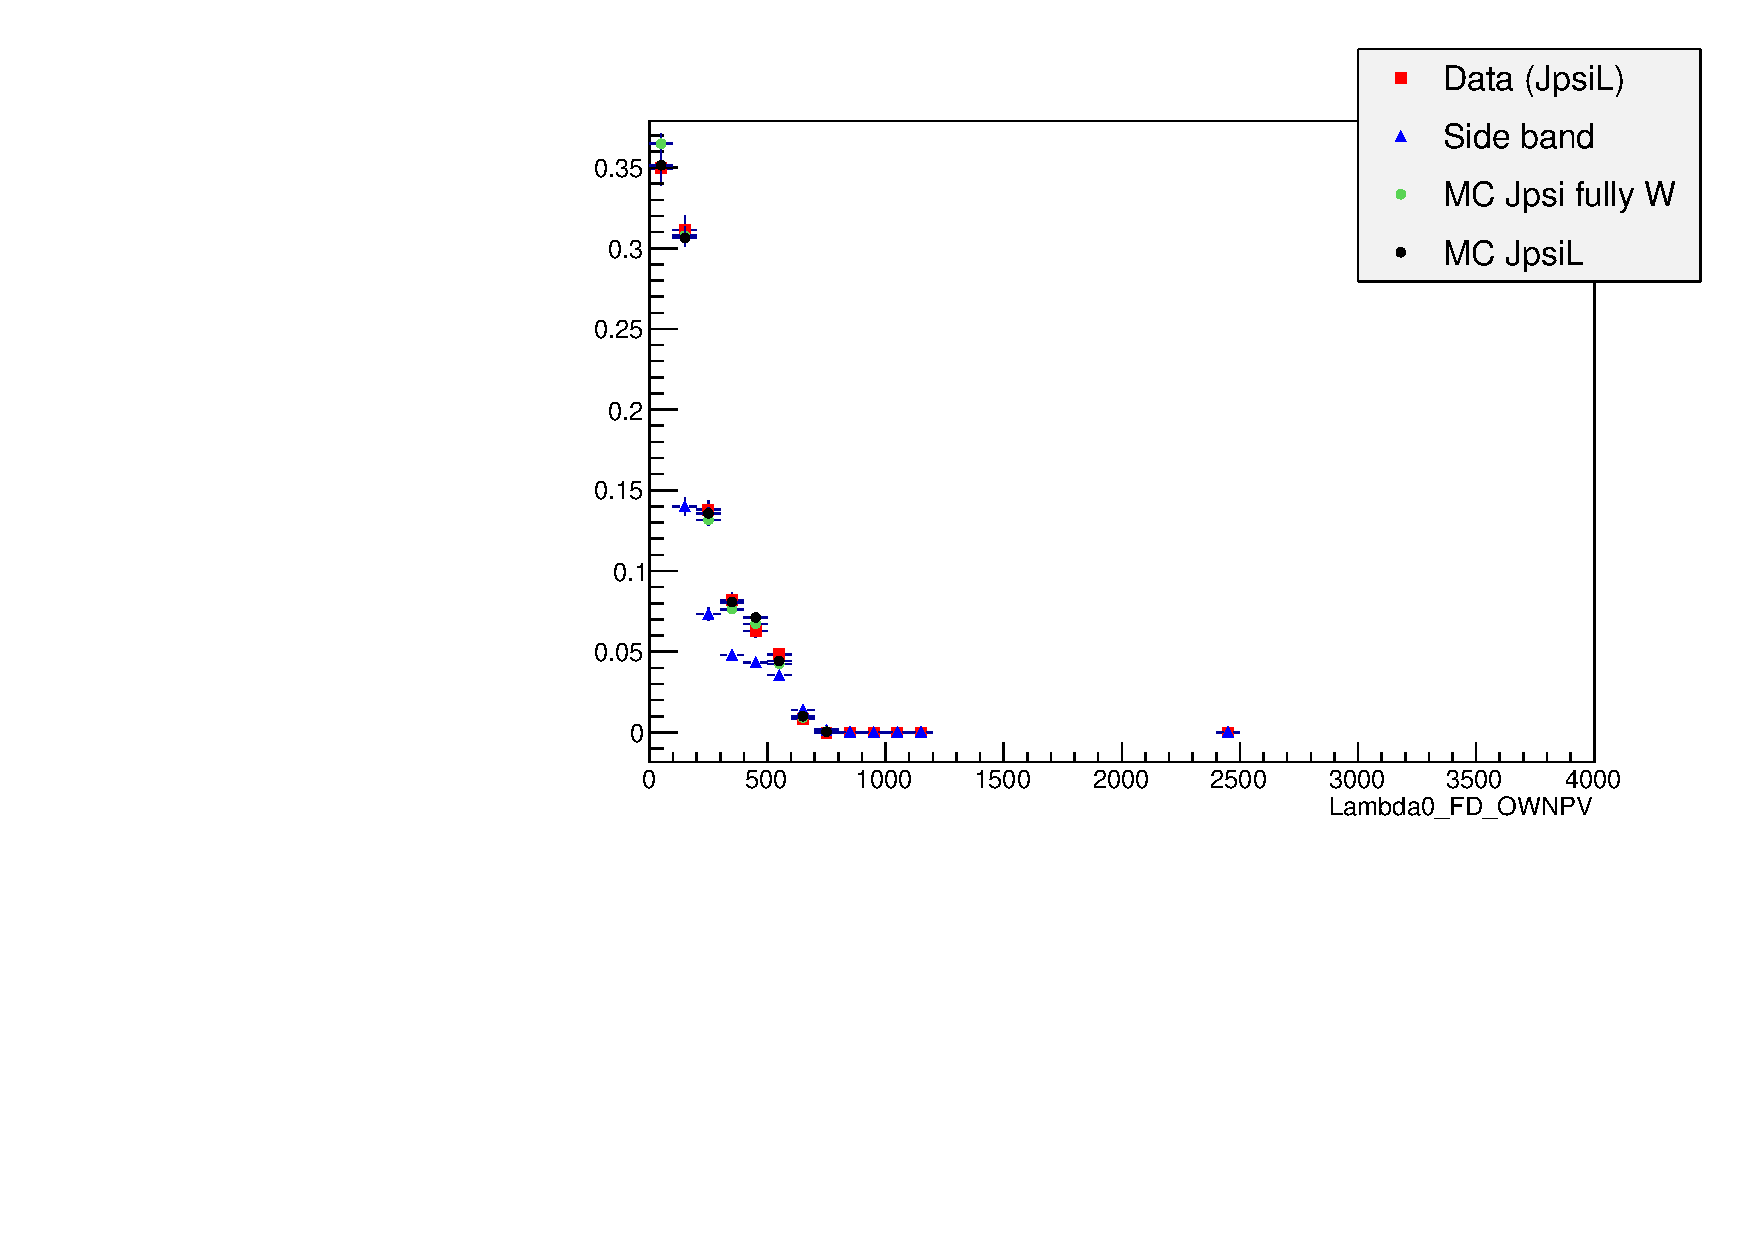
\includegraphics[width=0.48\textwidth]{Lmumu/figs/MC_data_comp/Lambda0_FD_OWNPV_plotLL.pdf}
%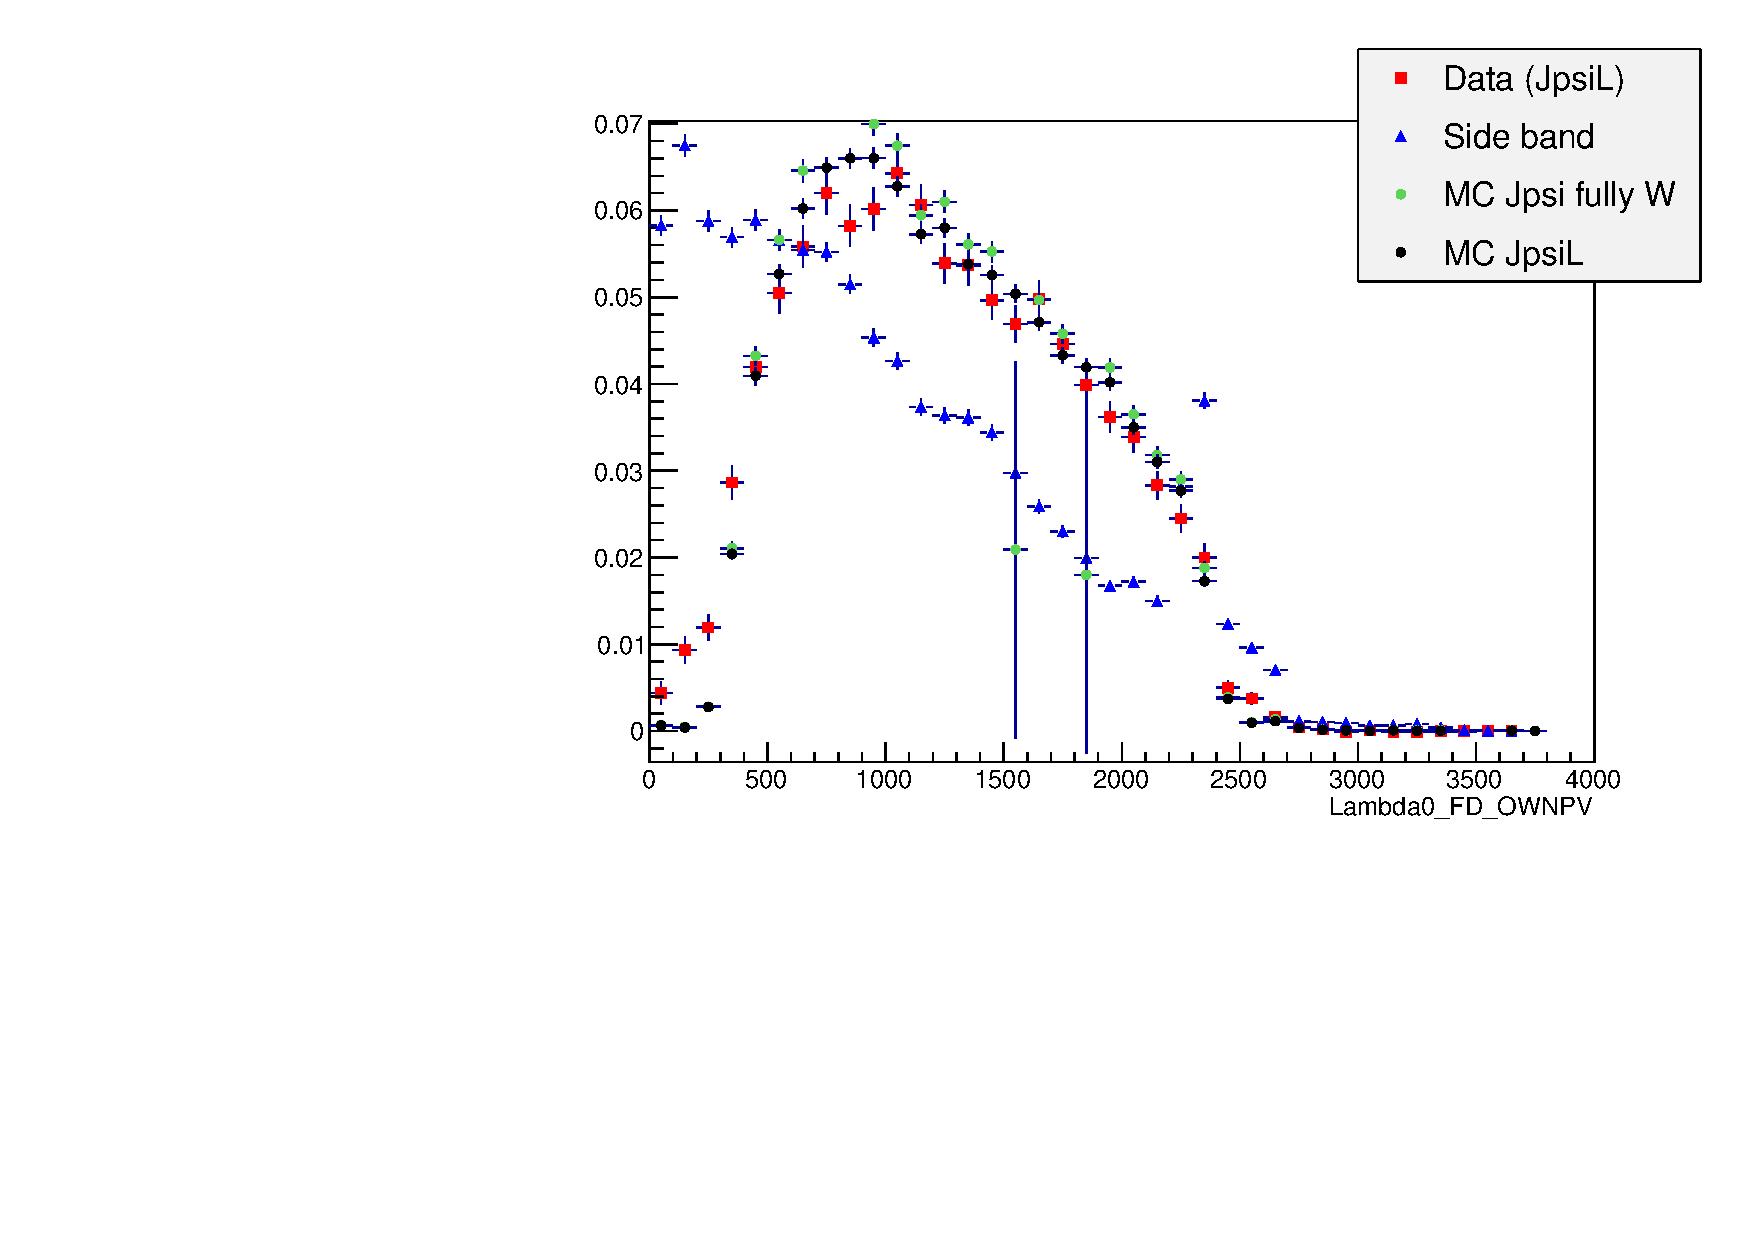
\includegraphics[width=0.48\textwidth]{Lmumu/figs/MC_data_comp/Lambda0_FD_OWNPV_plotDD.pdf}
%\caption{ Distributions of \Lz flight distance variable in MC, data signal and data background for LL (left) and DD (right) events.   }
%\end{figure}


%\begin{figure}[h!]
%\centering
%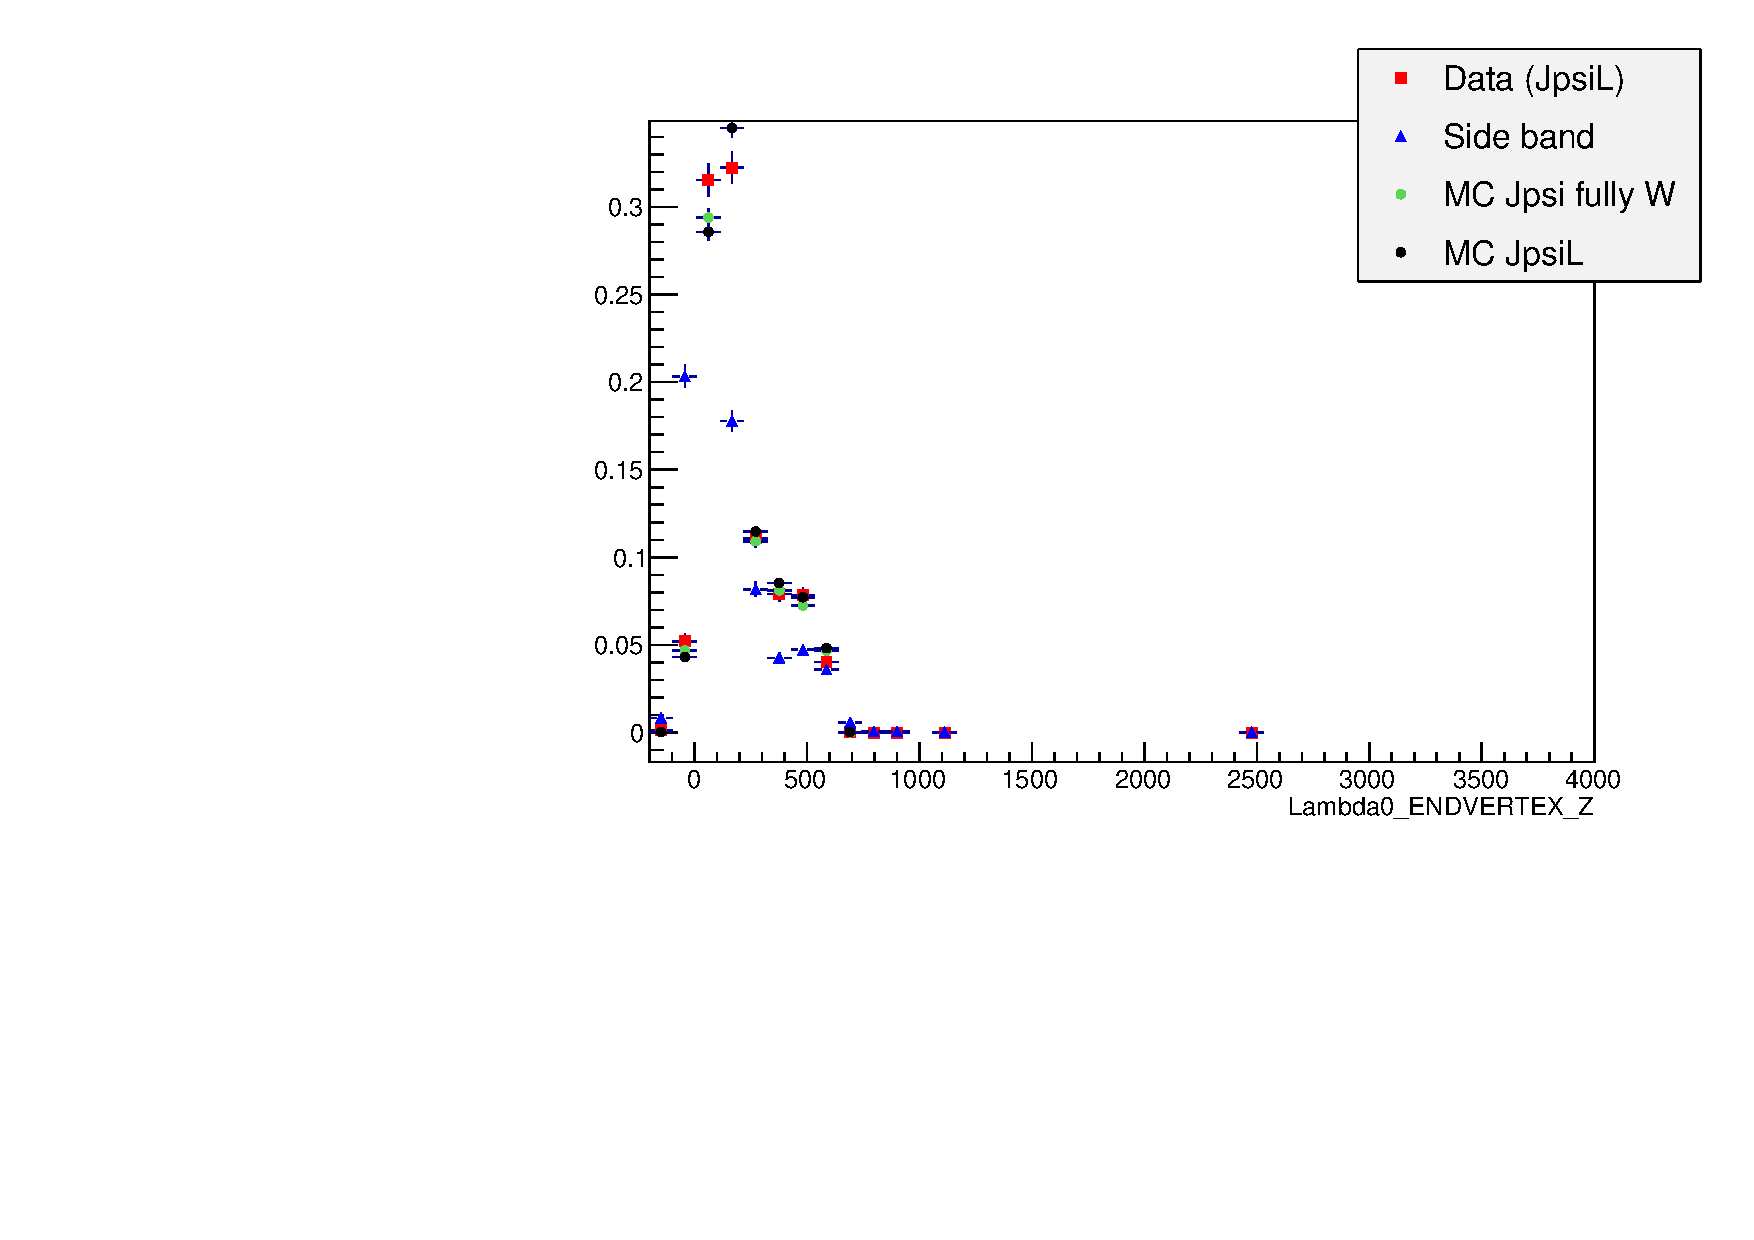
\includegraphics[width=0.48\textwidth]{Lmumu/figs/MC_data_comp/Lambda0_ENDVERTEX_Z_plotLL.pdf}
%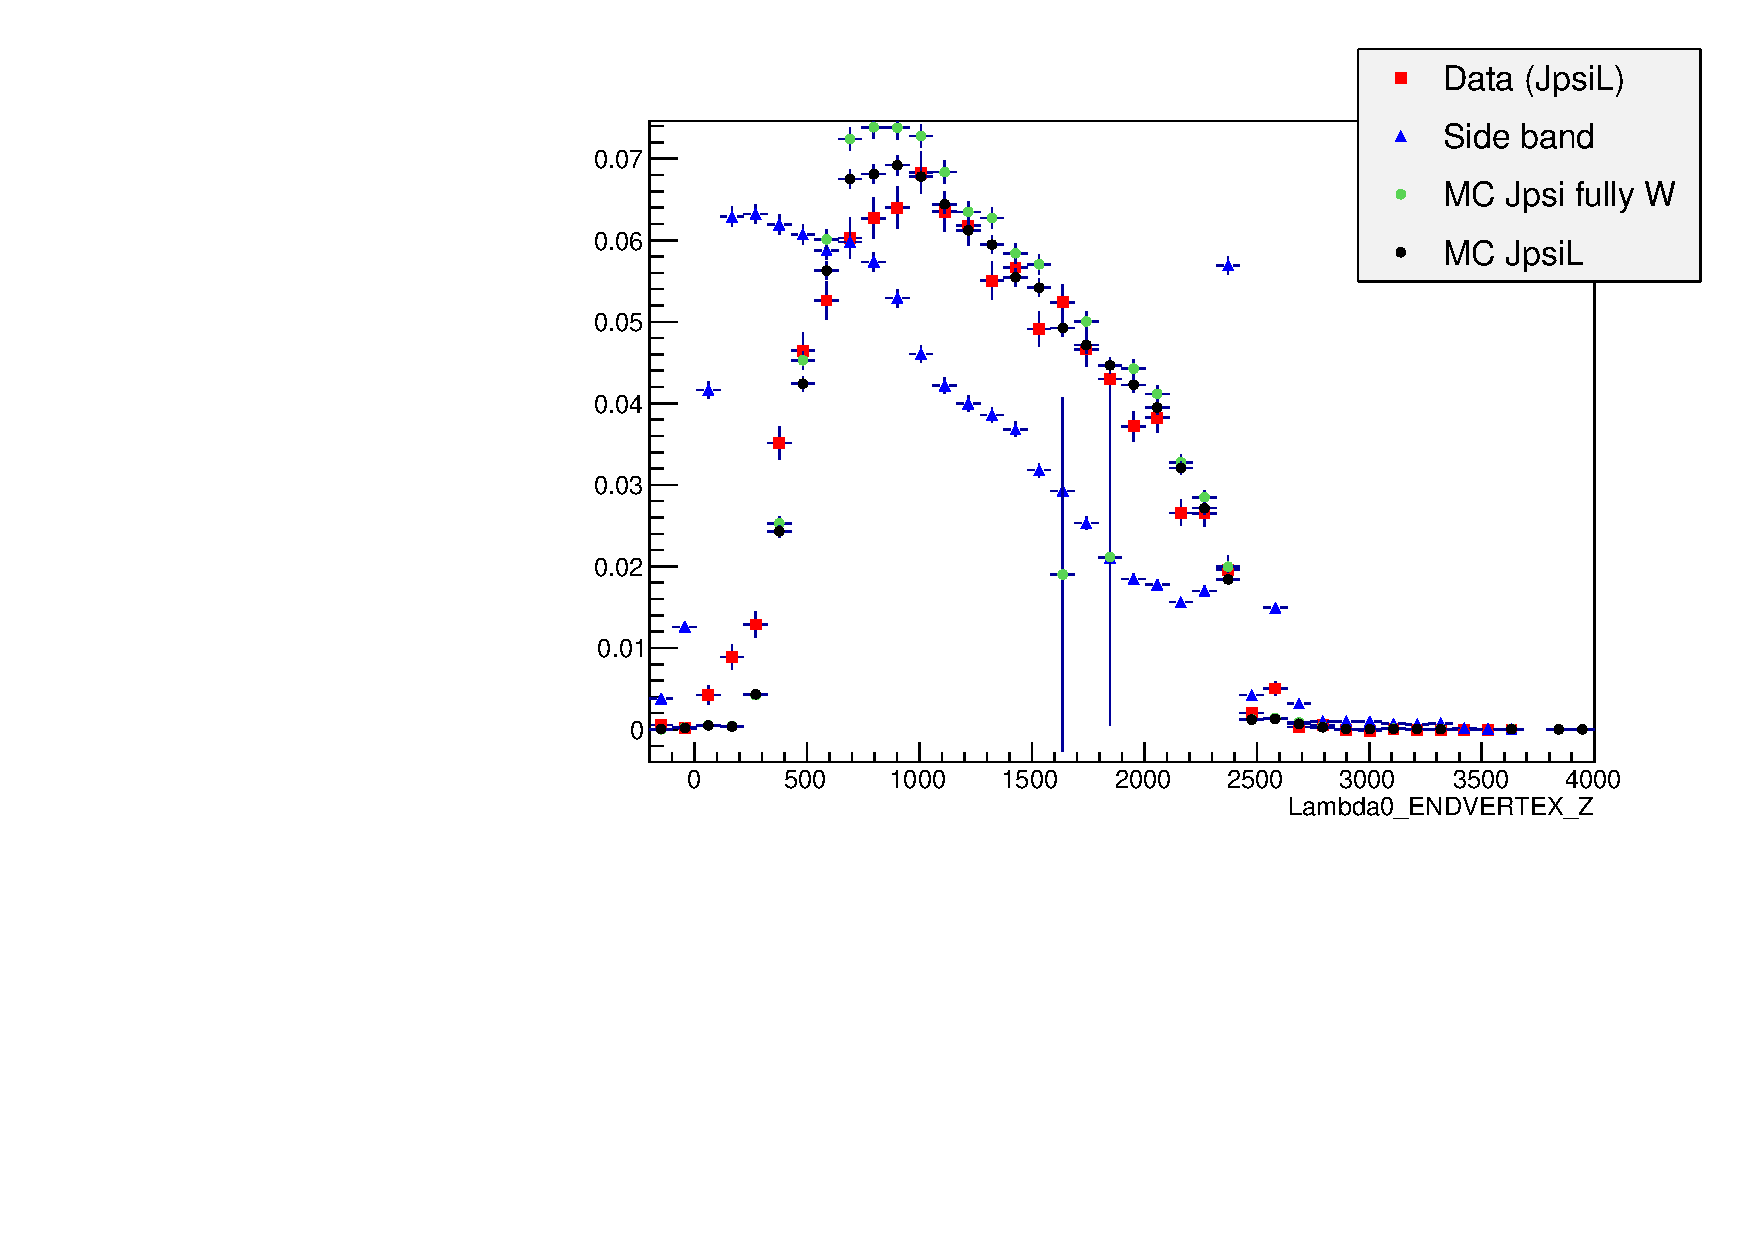
\includegraphics[width=0.48\textwidth]{Lmumu/figs/MC_data_comp/Lambda0_ENDVERTEX_Z_plotDD.pdf}
%\caption{ Distributions of \Lz vertex position ($z$ coordinate) variable in data and simulation for LL (left) and DD (right) events.   }
%\end{figure}




%\begin{figure}[h!]
%\centering
%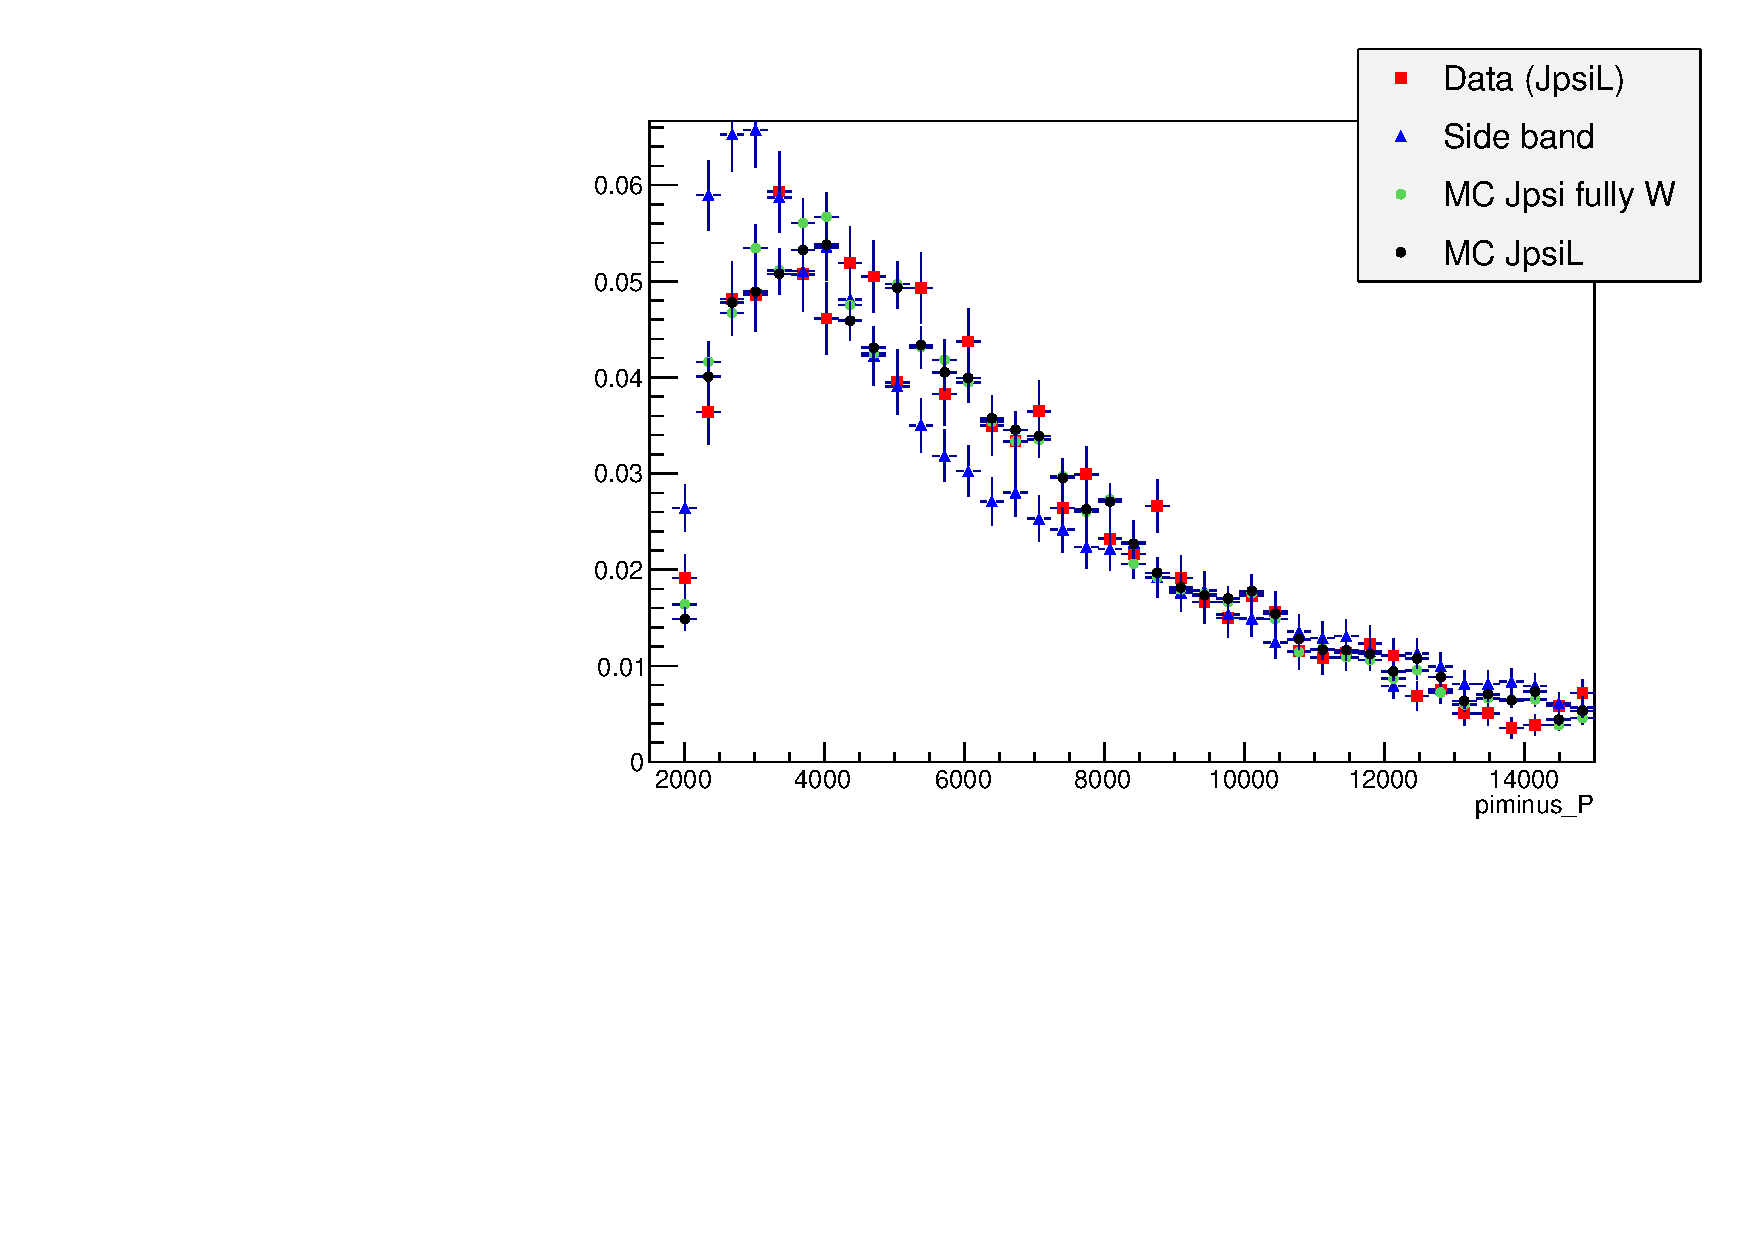
\includegraphics[width=0.48\textwidth]{Lmumu/figs/MC_data_comp/piminus_P_plotLL.pdf}
%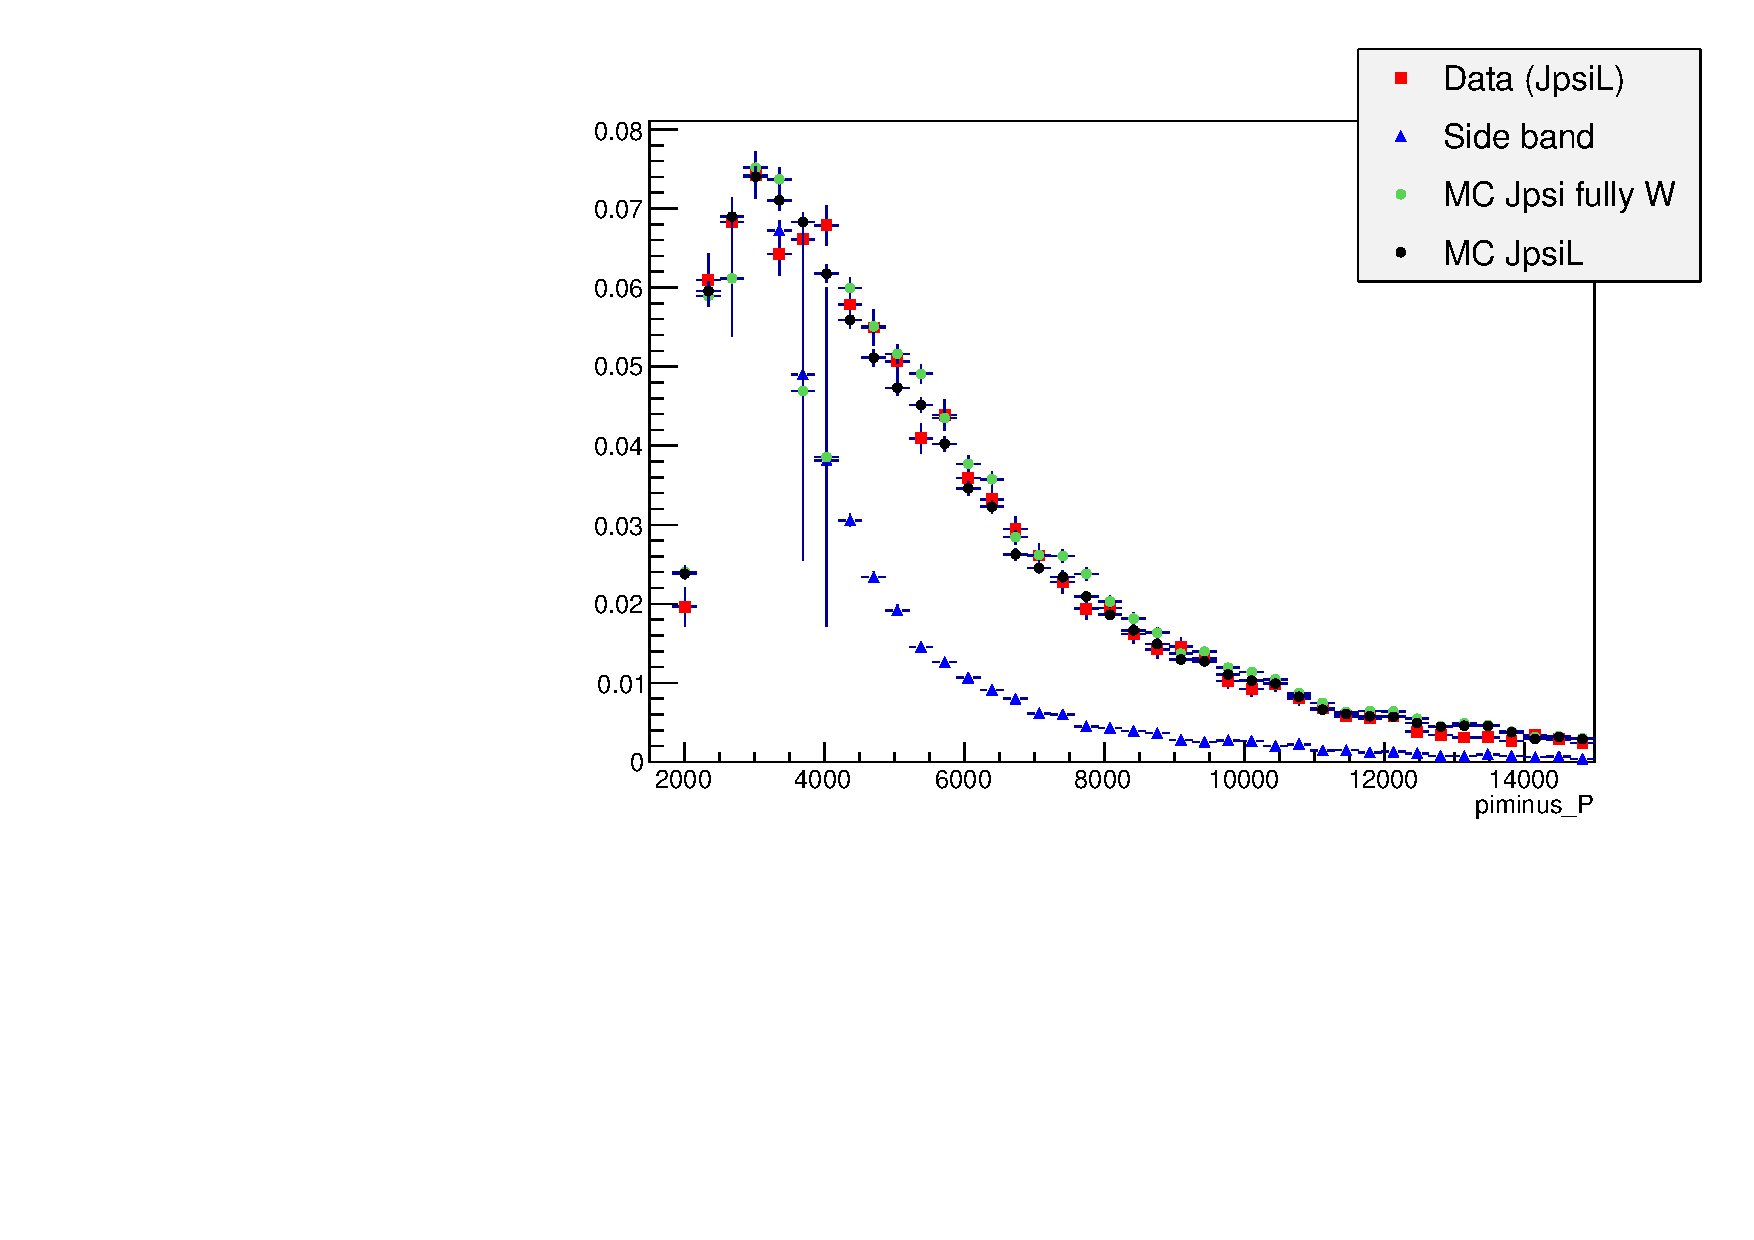
\includegraphics[width=0.48\textwidth]{Lmumu/figs/MC_data_comp/piminus_P_plotDD.pdf}
%\caption{ Distributions of pion momentum variable in data and simulation for LL (left) and DD (right) events.   }
%\end{figure}


\begin{figure}[h!]
\centering
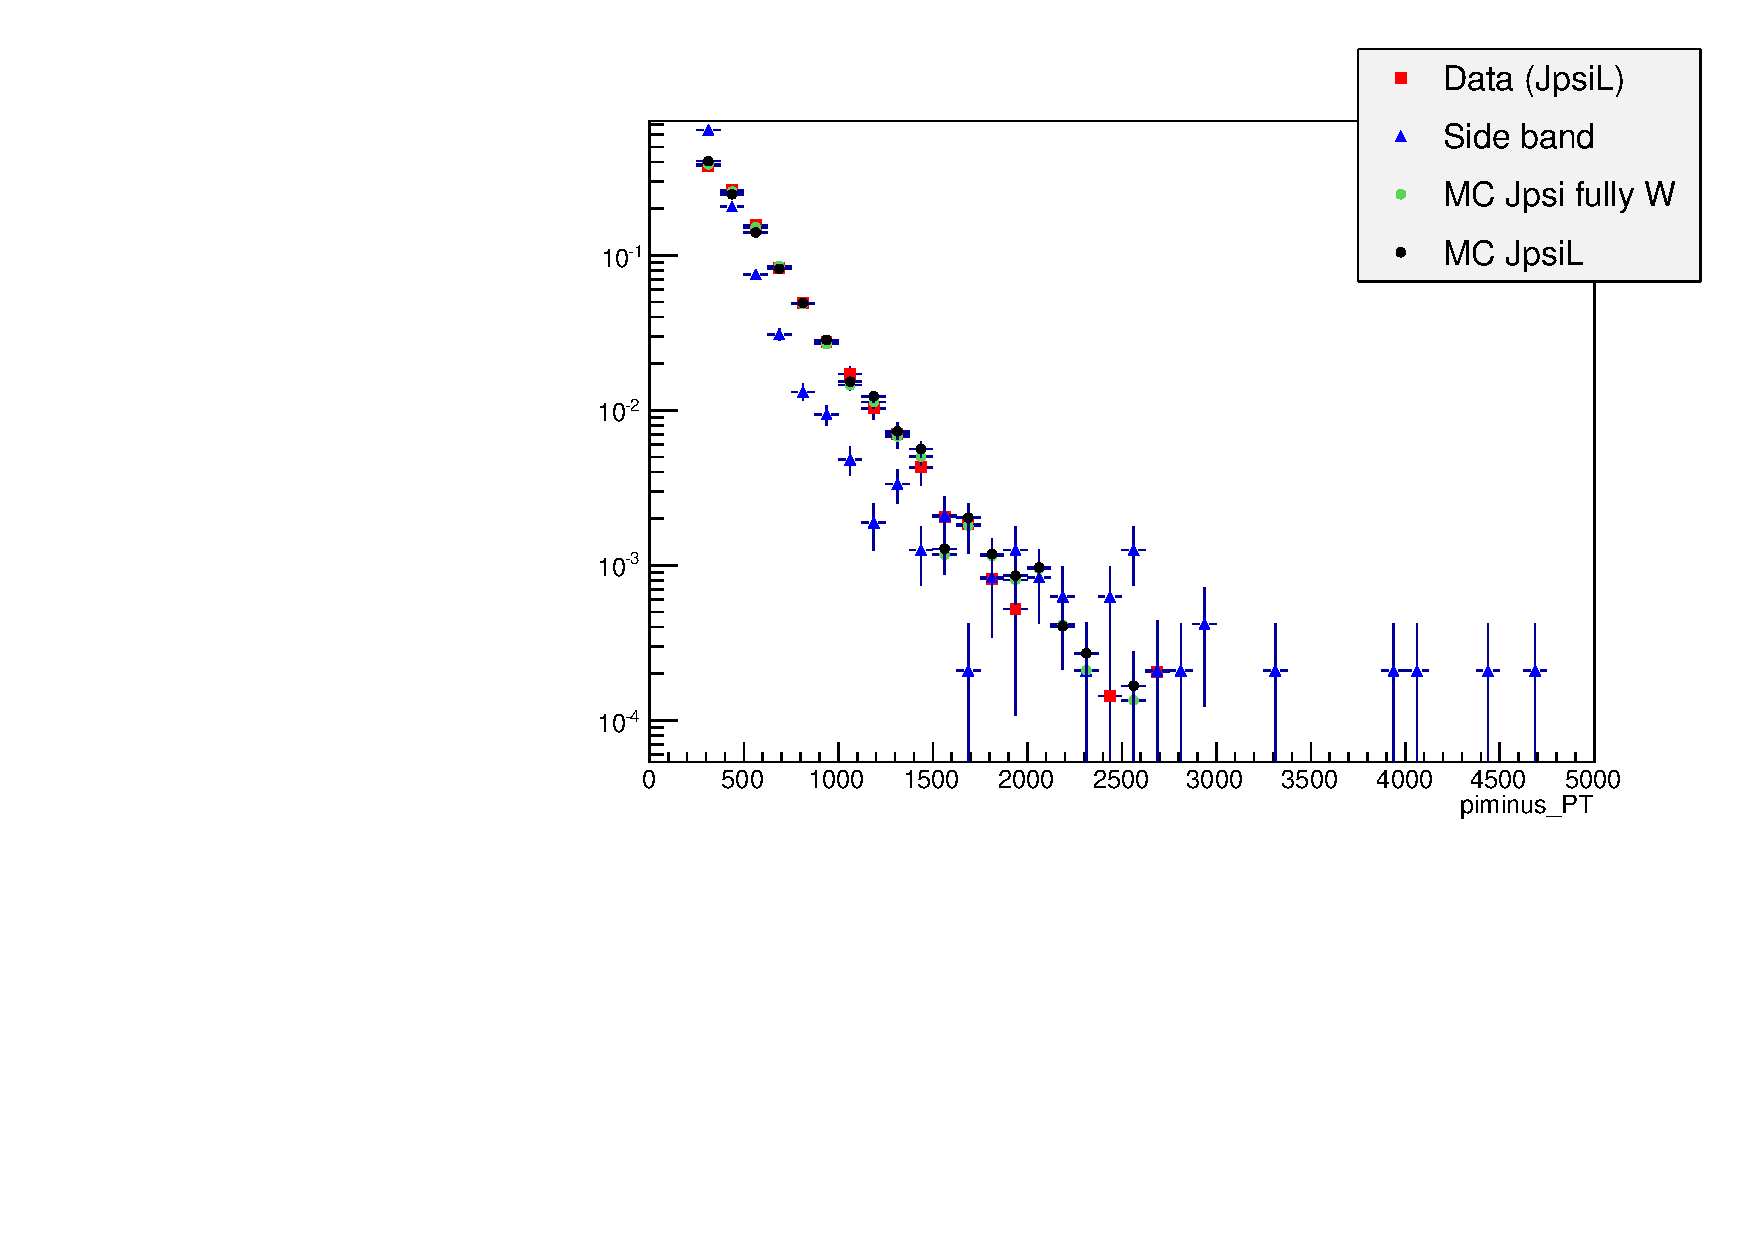
\includegraphics[width=0.48\textwidth]{Lmumu/figs/MC_data_comp/piminus_PT_plotLL.pdf}
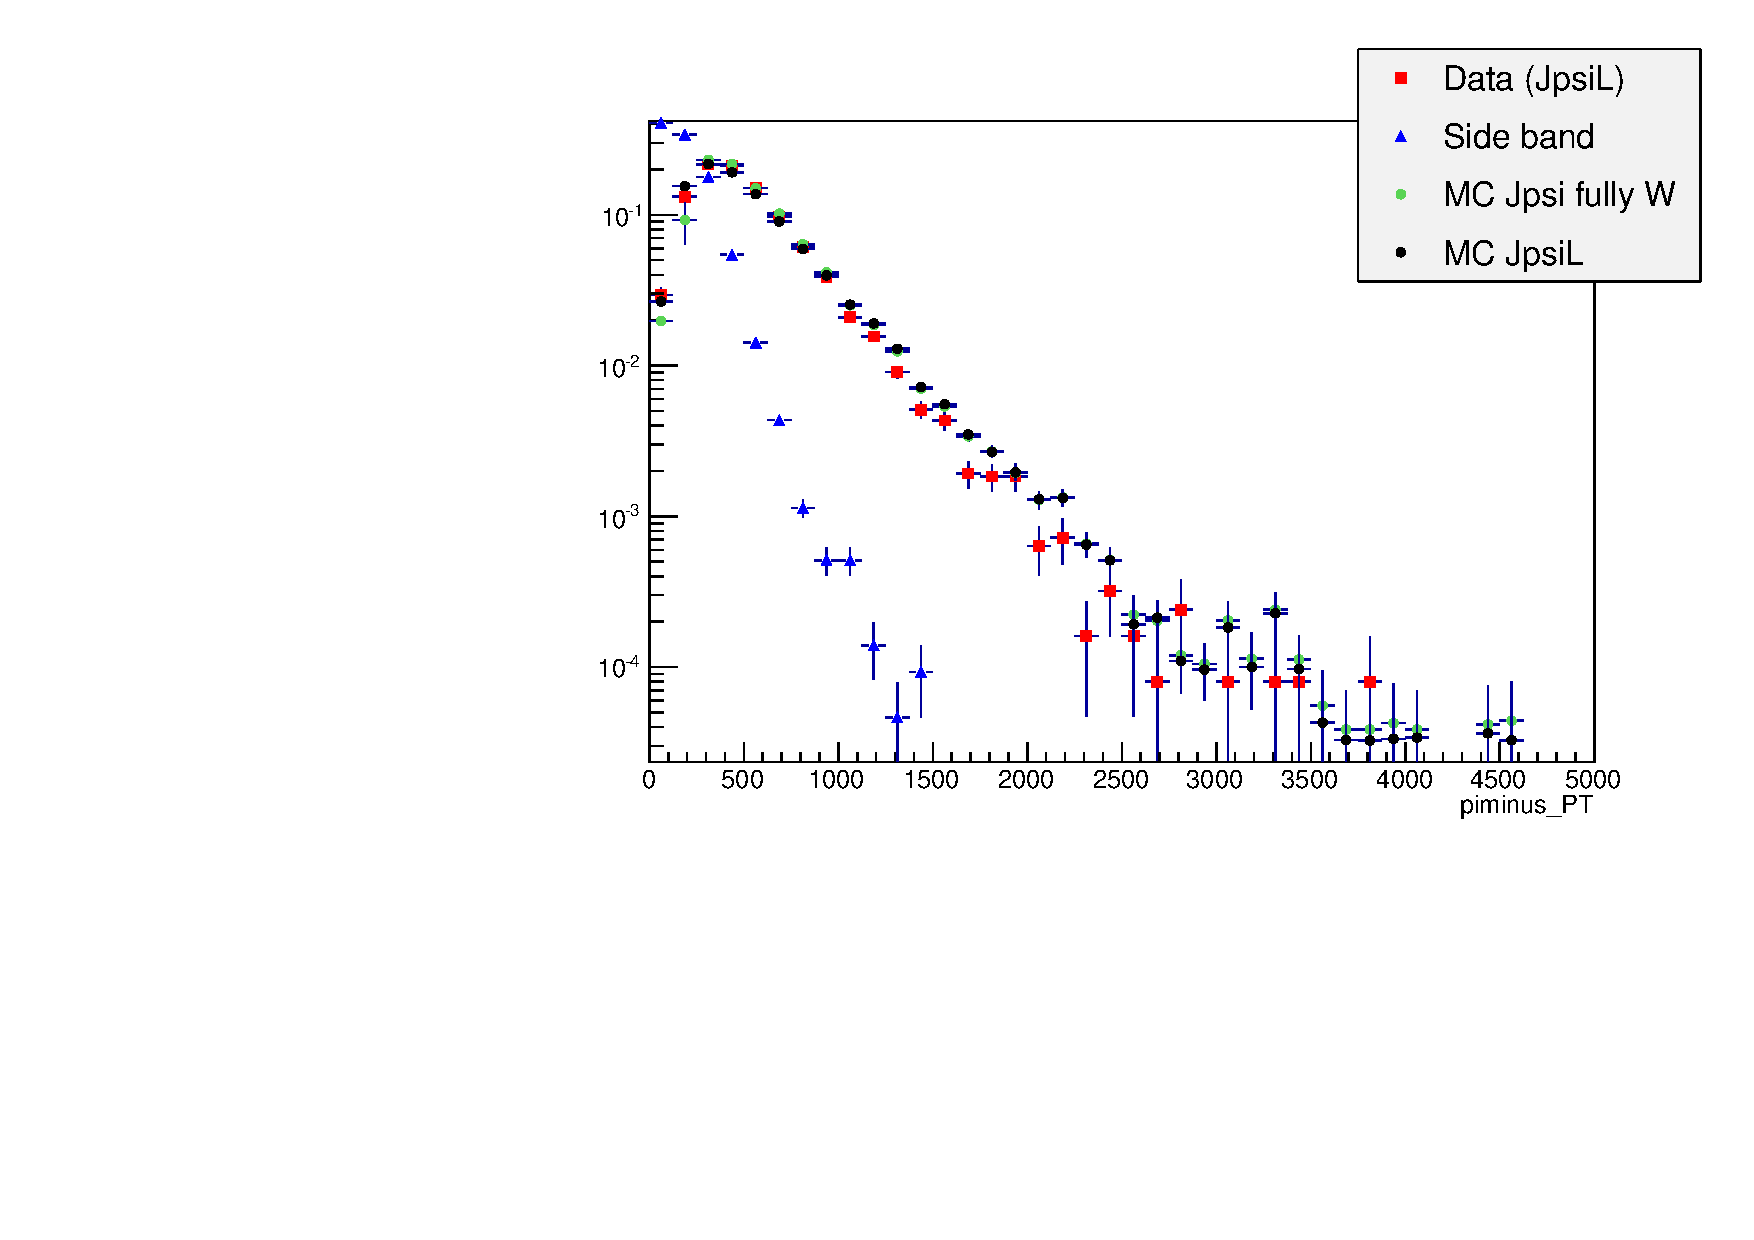
\includegraphics[width=0.48\textwidth]{Lmumu/figs/MC_data_comp/piminus_PT_plotDD.pdf}
\caption{ Distributions of pion transverse momentum variable in data and simulation for LL (left) and DD (right) events.   }
\end{figure}


%\begin{figure}[h!]
%\centering
%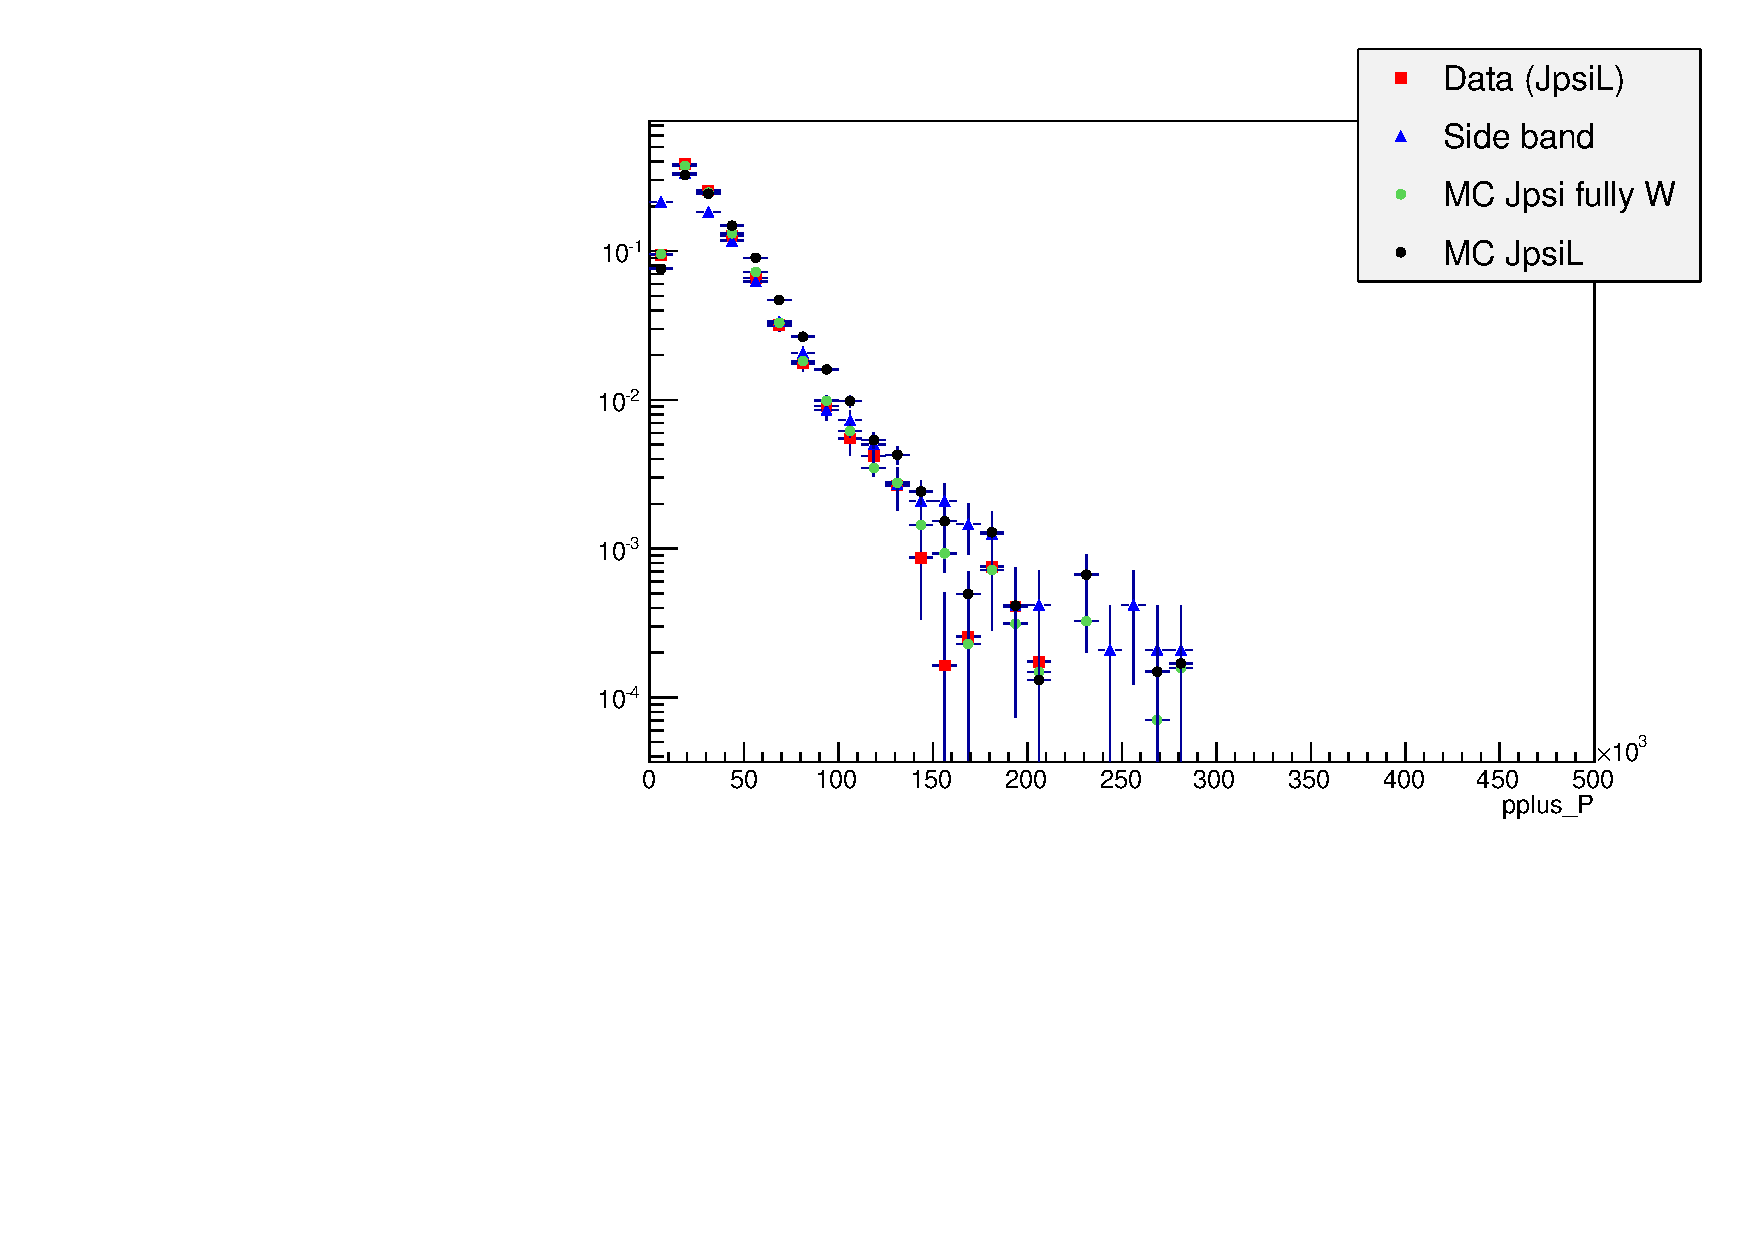
\includegraphics[width=0.48\textwidth]{Lmumu/figs/MC_data_comp/pplus_P_plotLL.pdf}
%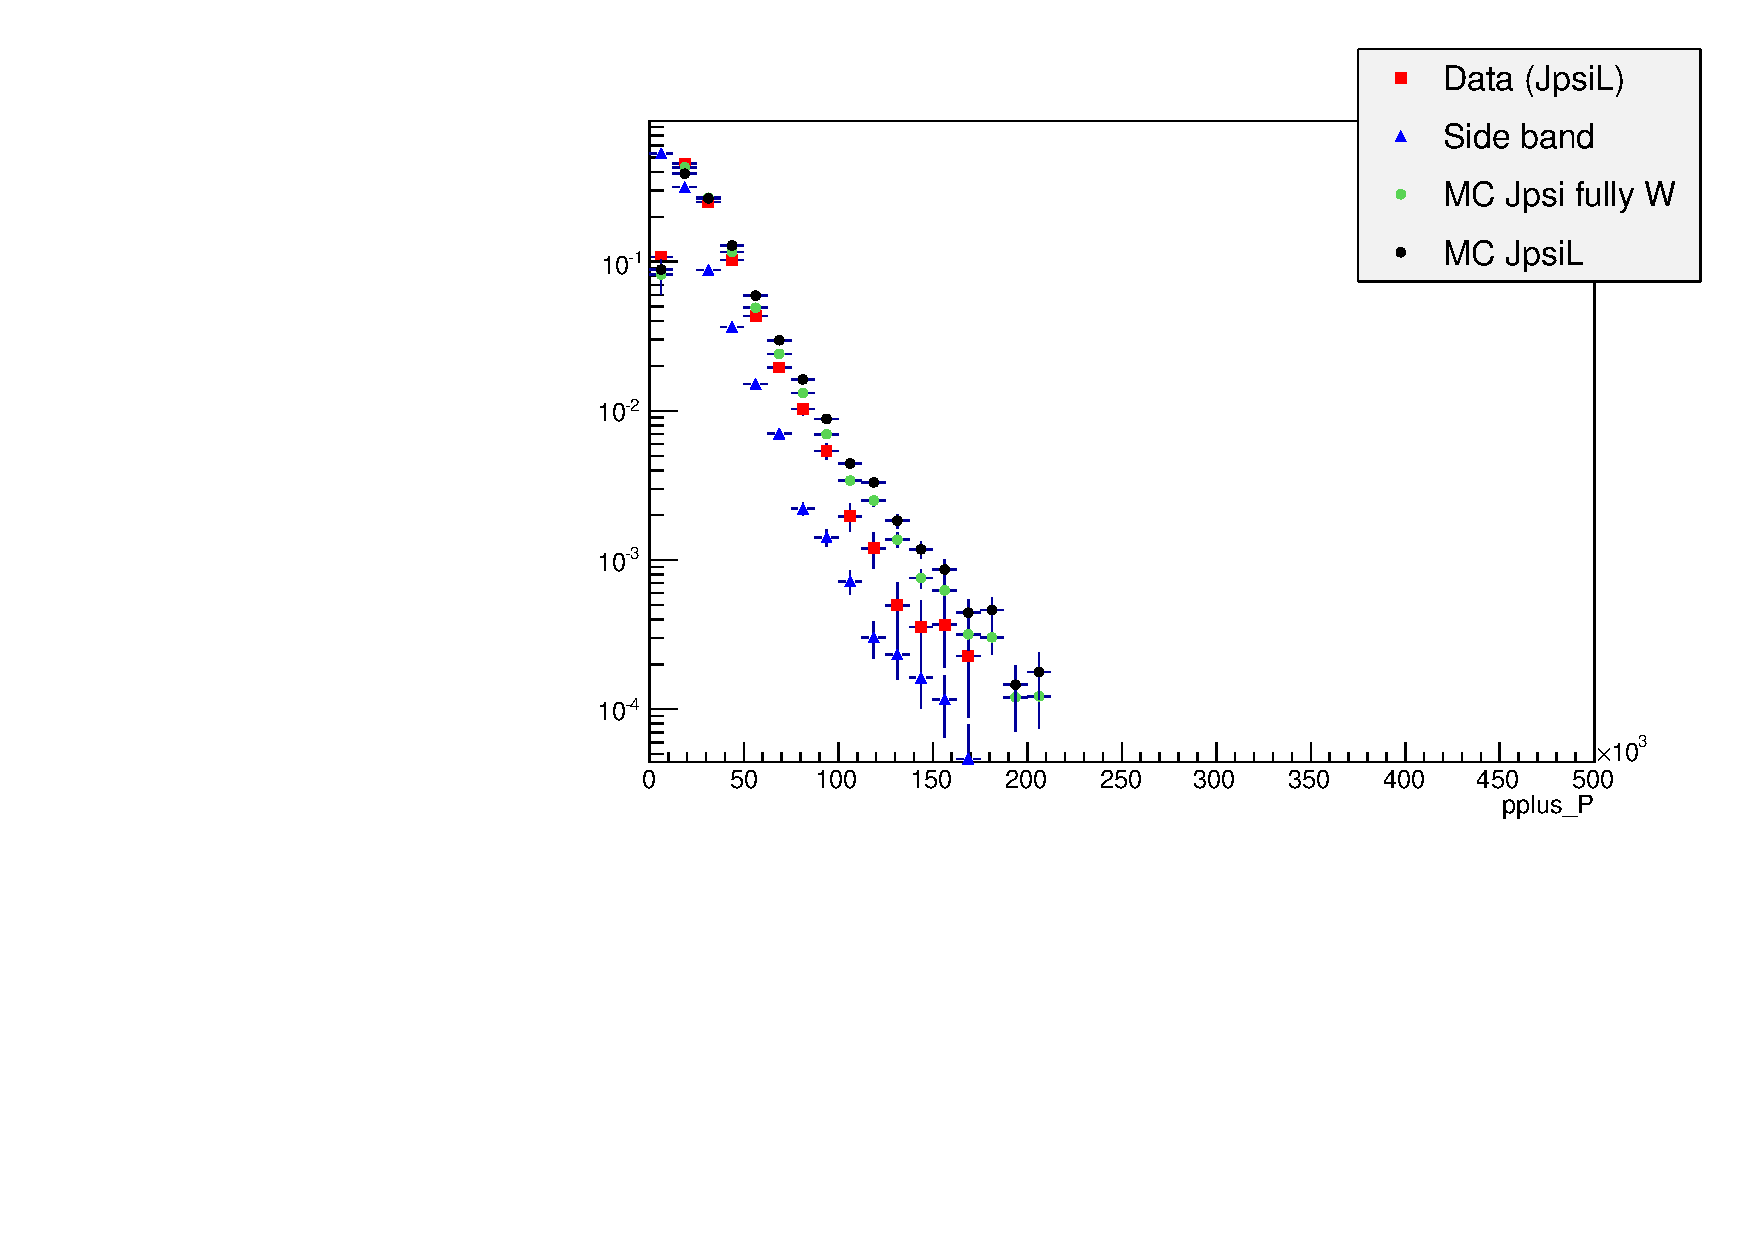
\includegraphics[width=0.48\textwidth]{Lmumu/figs/MC_data_comp/pplus_P_plotDD.pdf}
%\caption{ Distributions of proton momentum variable in MC, data signal and data background for LL (left) and DD (right) events.   }
%\end{figure}


\begin{figure}[h!]
\centering
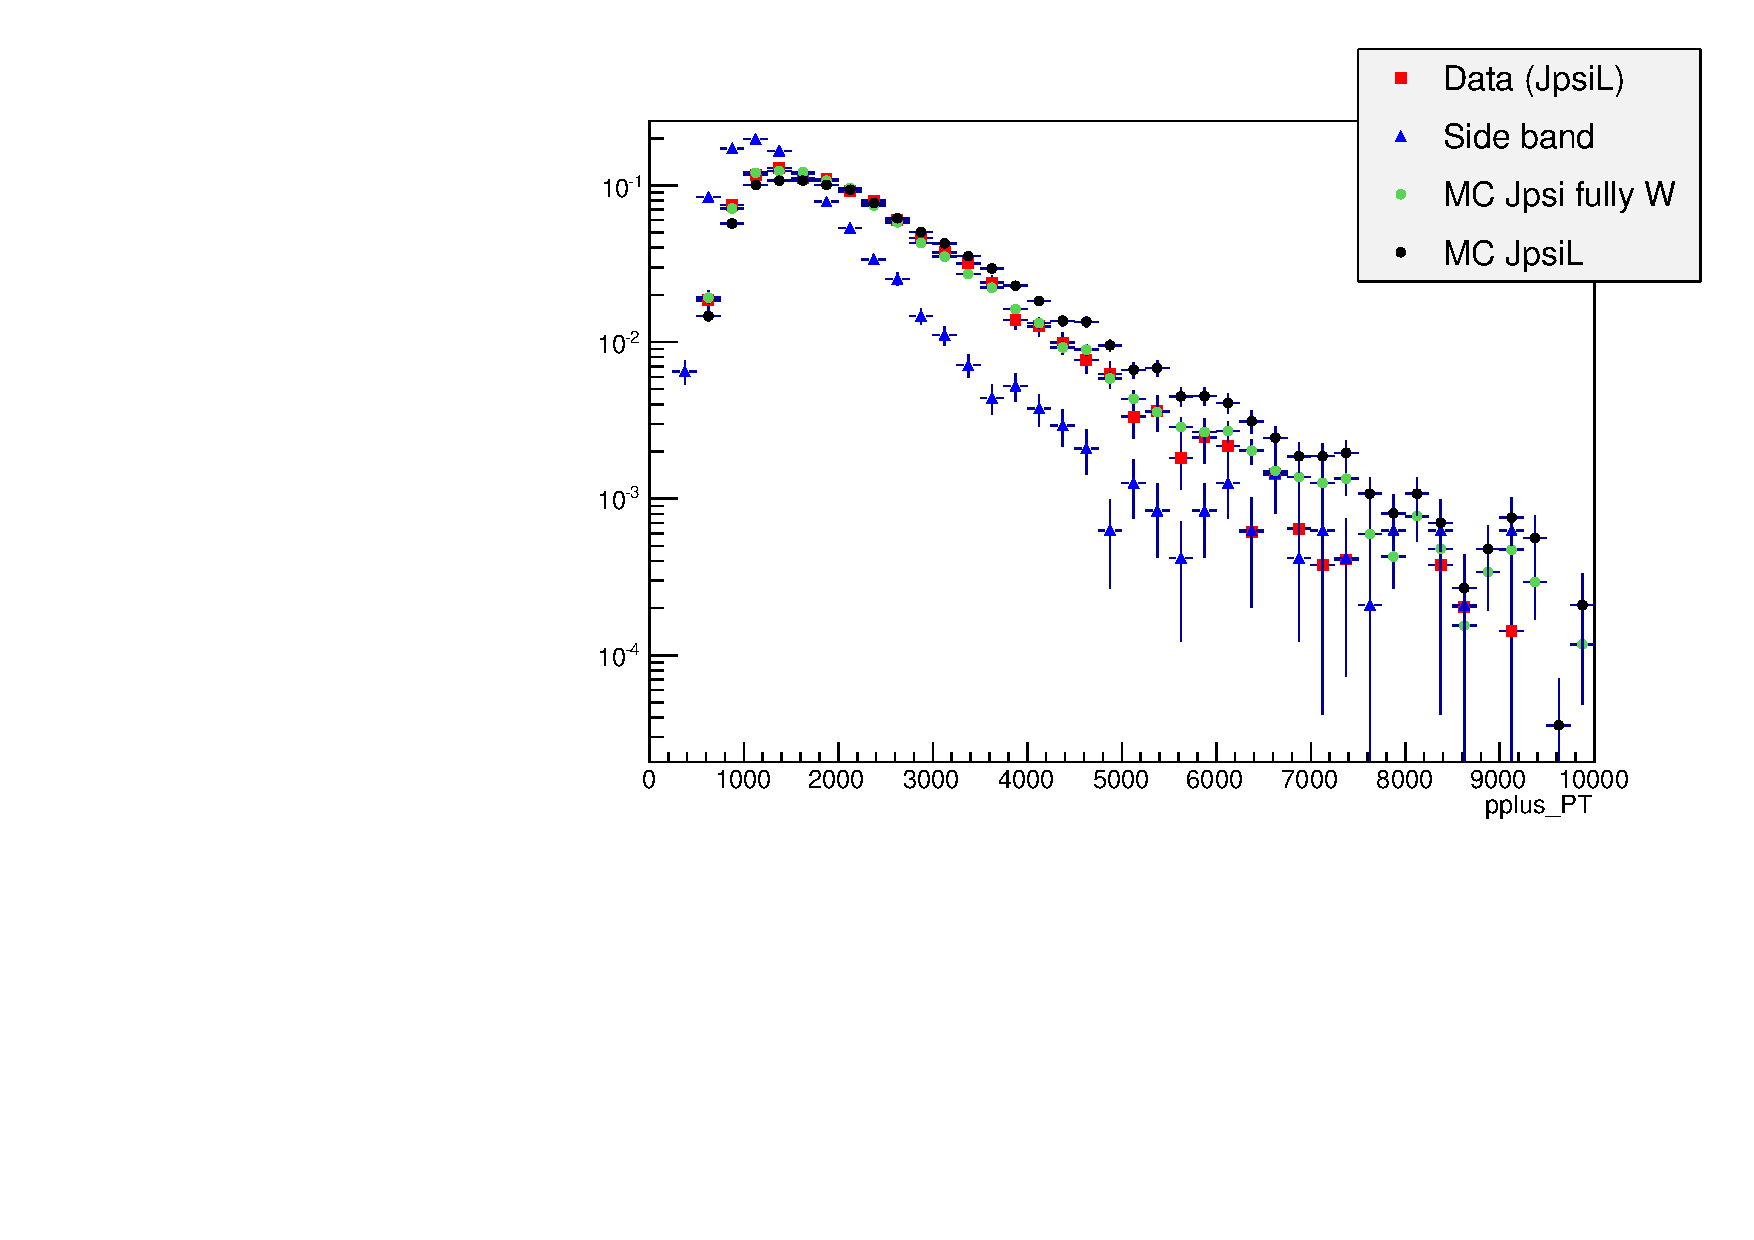
\includegraphics[width=0.48\textwidth]{Lmumu/figs/MC_data_comp/pplus_PT_plotLL.pdf}
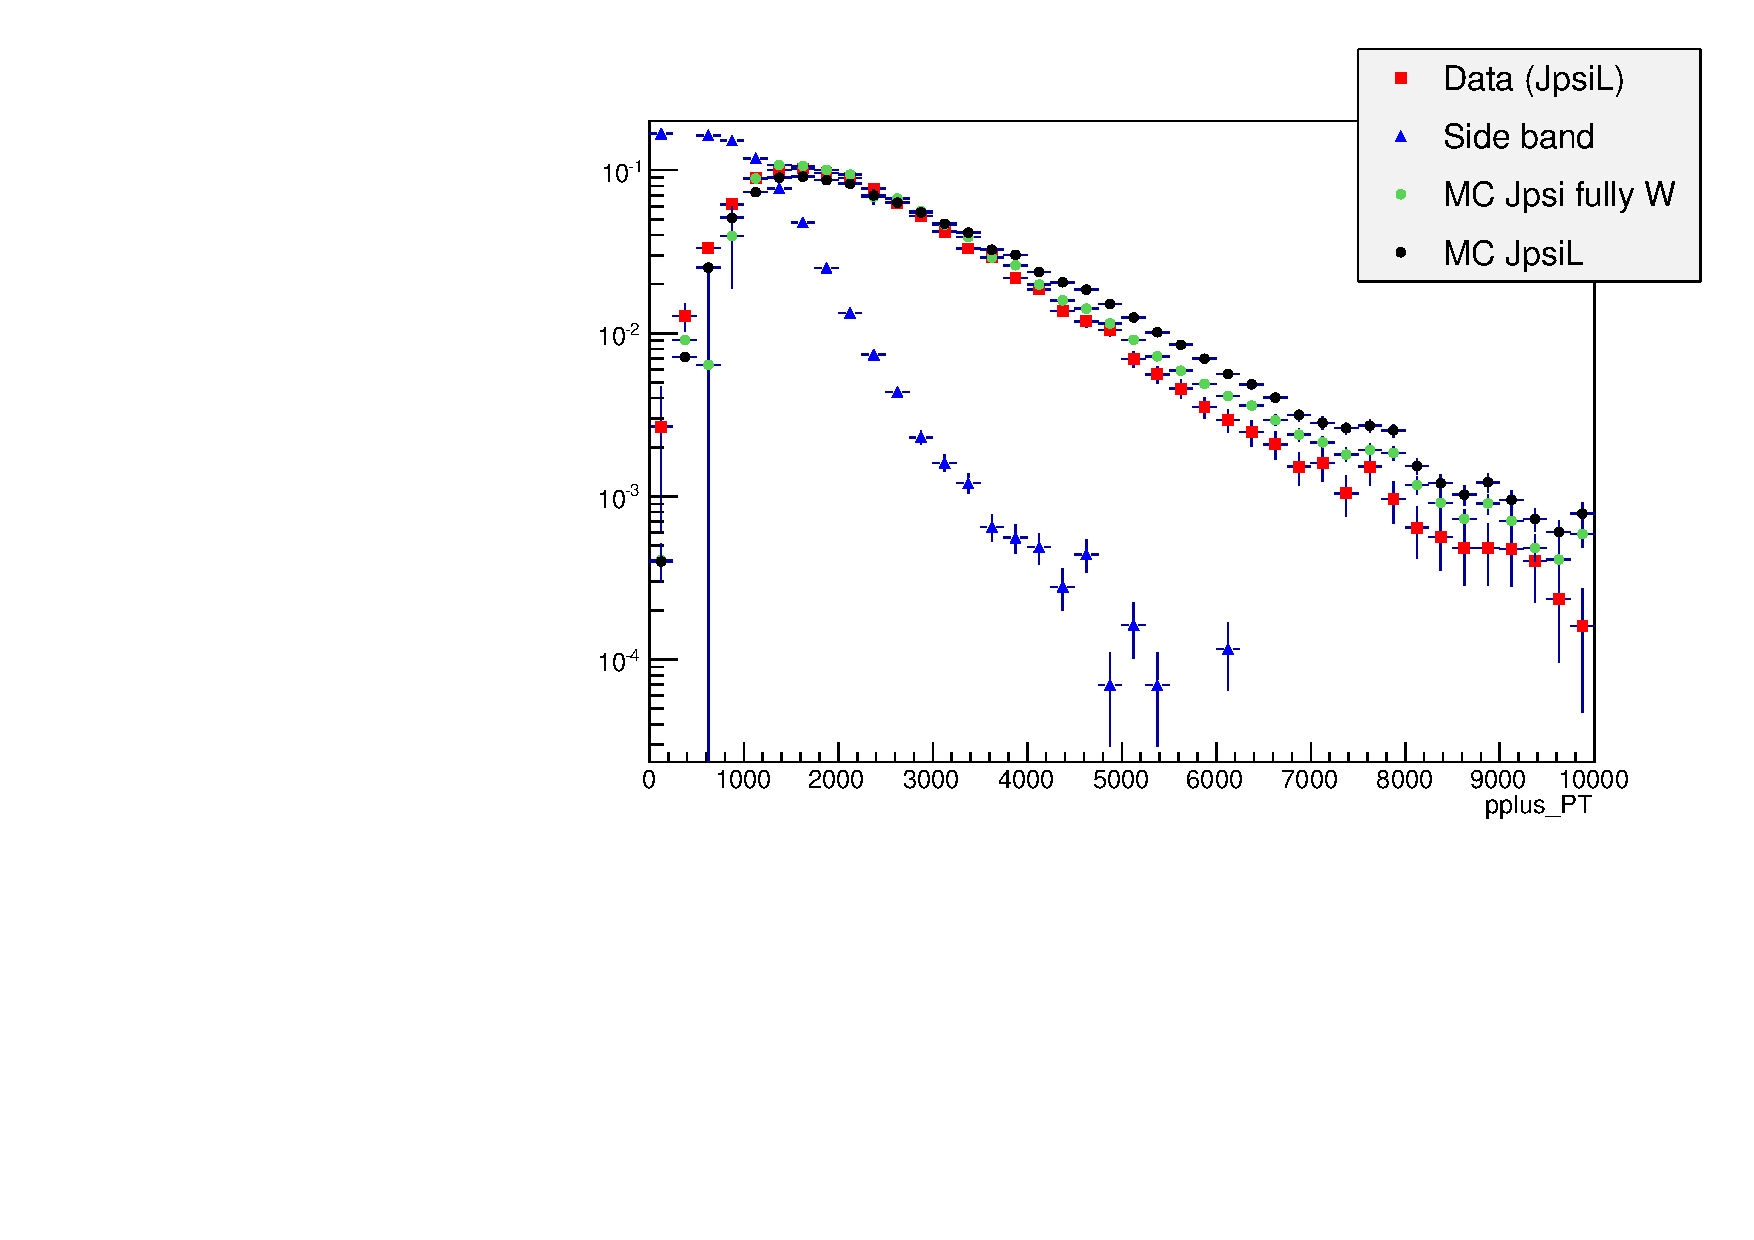
\includegraphics[width=0.48\textwidth]{Lmumu/figs/MC_data_comp/pplus_PT_plotDD.pdf}
\caption{ Distributions of proton transverse momentum variable in data and simulation for LL (left) and DD (right) events.   }
\end{figure}


%\begin{figure}[h!]
%\centering
%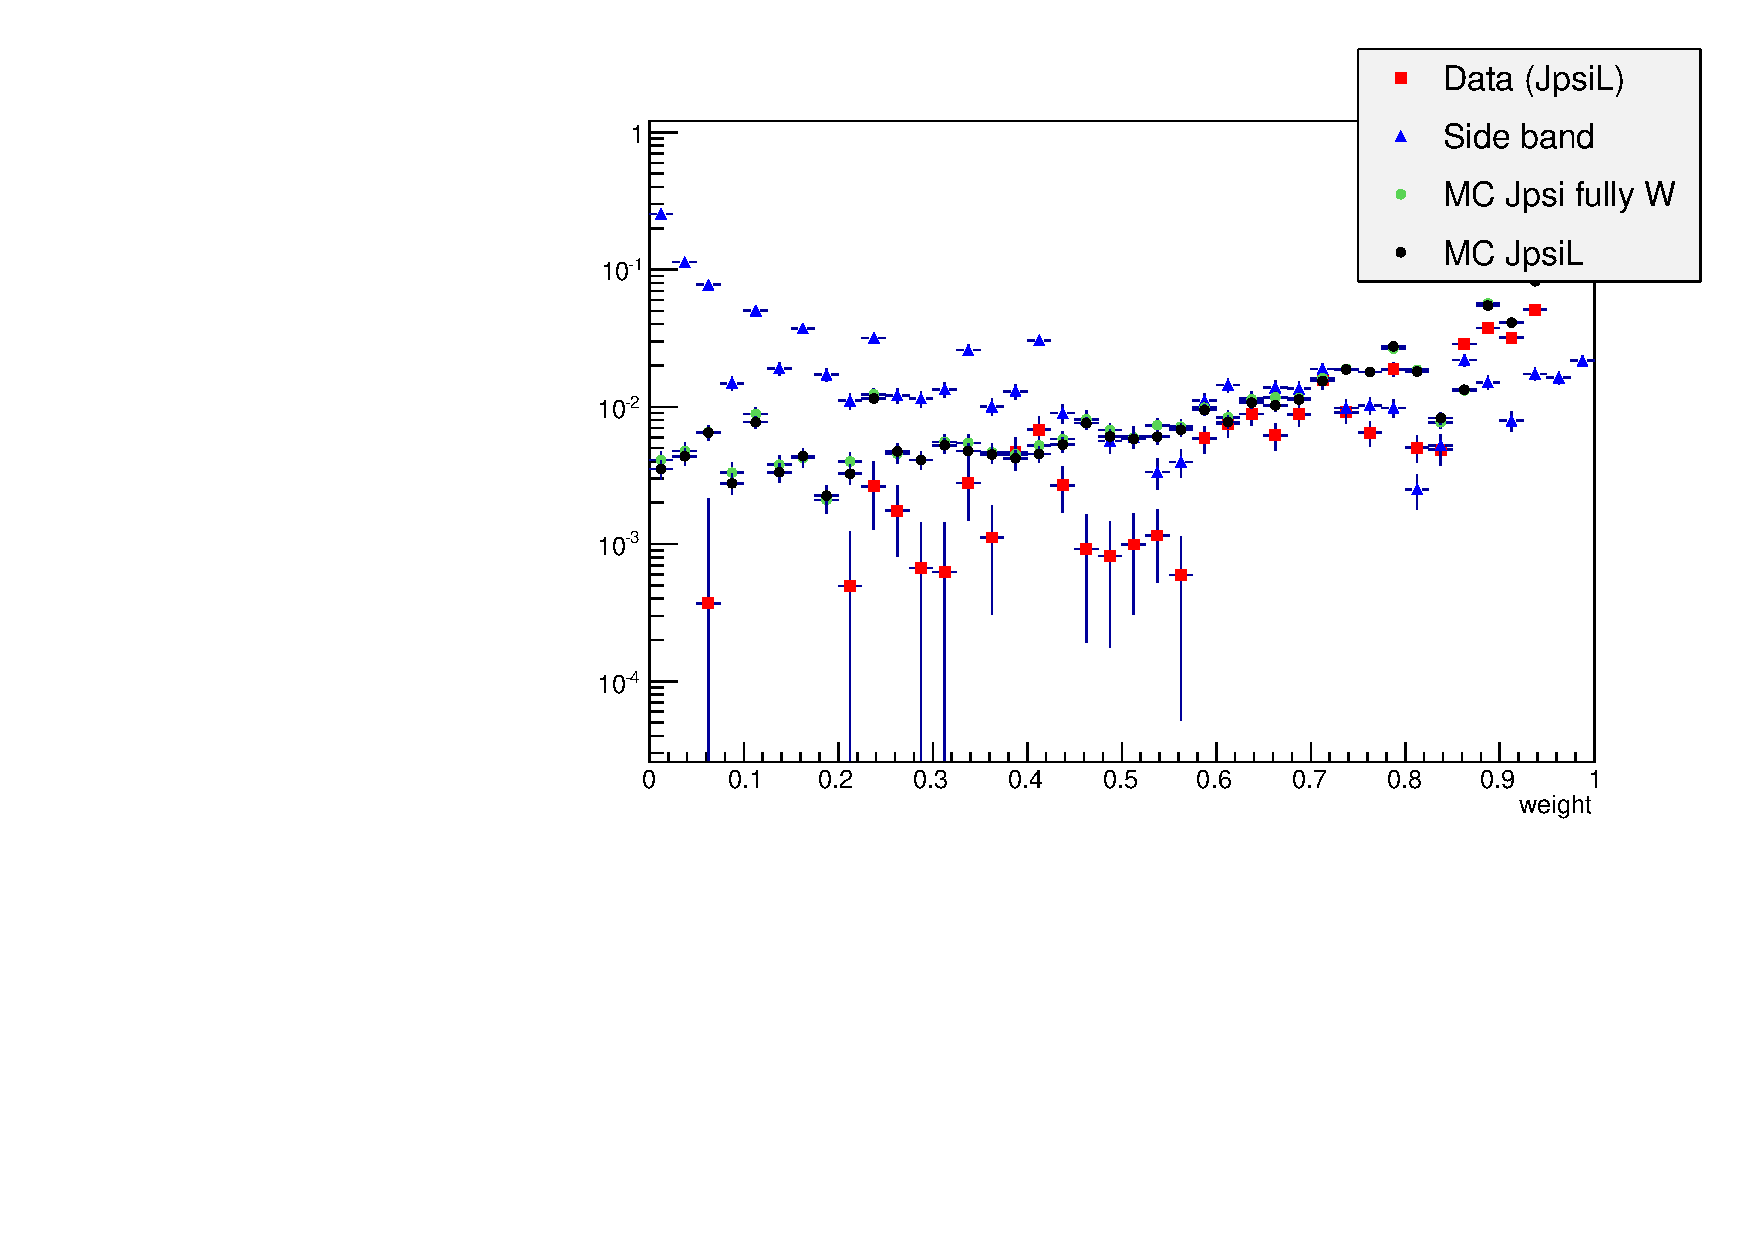
\includegraphics[width=0.48\textwidth]{Lmumu/figs/MC_data_comp/weight_plotLL.pdf}
%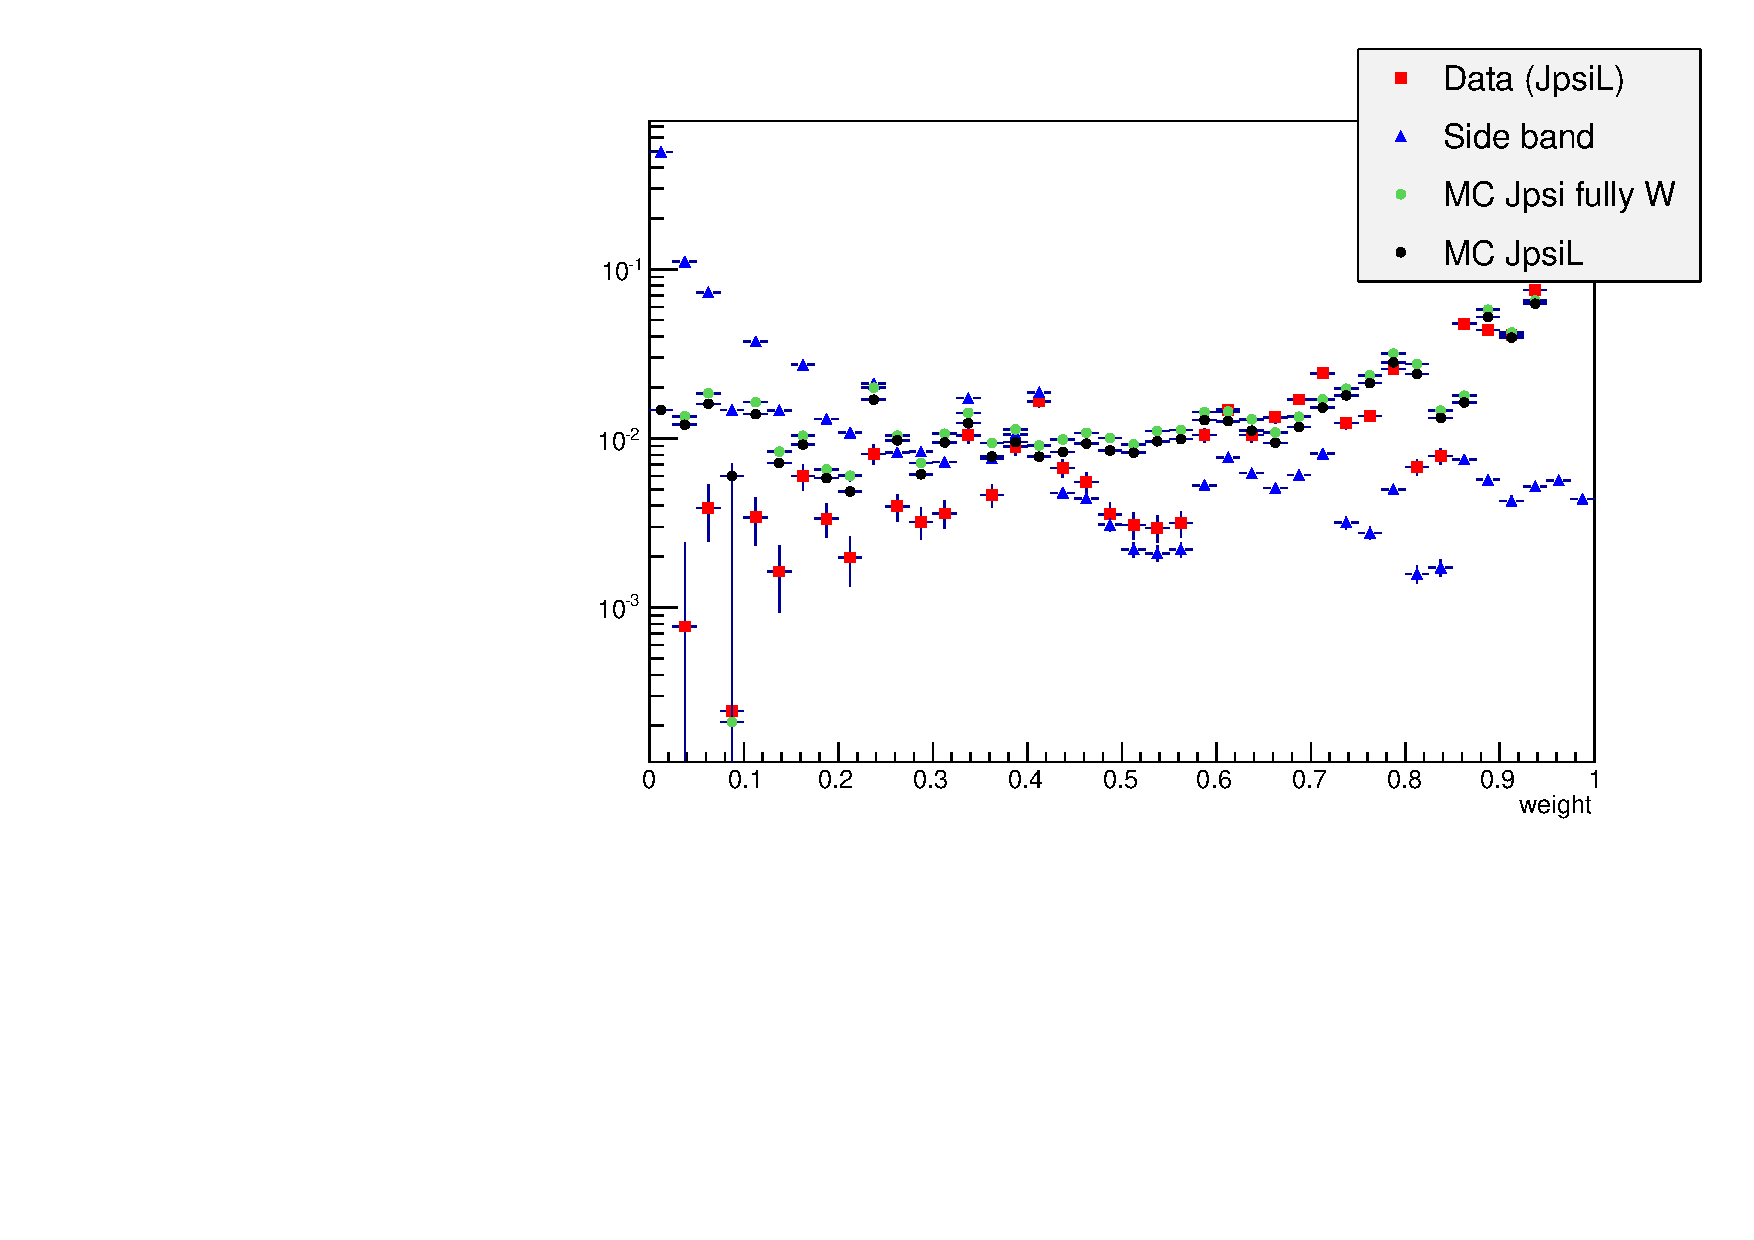
\includegraphics[width=0.48\textwidth]{Lmumu/figs/MC_data_comp/weight_plotDD.pdf}
%\caption{ Distributions of NN output variable in MC, data signal and data background for LL (left) and DD (right) events.   }
%\end{figure}





\clearpage
